% !TEX options=--shell-escape
\documentclass[a4paper]{book}
\usepackage[russian]{babel}
\usepackage[left=2cm,right=2cm,top=2cm,bottom=2cm,bindingoffset=0cm]{geometry}

\usepackage[poster]{tcolorbox}
\usepackage{longtable}

\tolerance=1
\emergencystretch=\maxdimen
\hyphenpenalty=10000
\hbadness=10000

\newcommand{\trouble}[8]{
\begin{center}
\begin{tabular}{ |p{2.7cm}|p{12cm}| }
\hline
\textbf{Результат проверки Неприятностей} & \textbf{Последствия}
\\ \hline
19-20 & \textbf{#1. }#2
\\ \hline
13-18 & \textbf{#3. }#4
\\ \hline
7-12 & \textbf{#5. }#6
\\ \hline
1-6 & \textbf{#7. }#8
\\ \hline
\end{tabular}
\end{center}
}

\newcommand{\troubleControl}{герой должен совершить проверку \textit{Неприятностей под Контролем} }
\endinput
\troubleControl
\trouble
{}%no sweat name
{}%no sweat description
{}%tough day name
{}%tough day description
{}%we have trouble name
{}%we have trouble description
{}%fiasco name
{}%fiasco description

\newcommand{\tbd}{\textcolor{orange}{\textbf{\textit{TBD}}}}
\newcommand{\err}{\textcolor{red}{\textbf{\textit{ERR}}}}
\newcommand{\genAndGet}[1]{\input{|python3 scripts/genFromJson.py #1}\input{scripts/output/#1}}

\begin{document}
\tableofcontents
\chapter*{ВСТУПЛЕНИЕ}
\addcontentsline{toc}{chapter}{ВСТУПЛЕНИЕ}
Эта игра о Судьбе, которая управляет всем, кроме свободной воли. Эта игра о победах, ведущих к поражениям, и о поражениях, ведущих к победам. Эта игра о борьбе с самим собой и о Нитях, протянутых над бездной. Эта игра о том, как просто отнять чужую жизнь, как легко расстаться со своей и как сложно порой избежать и того, и другого.
Вам предстоит выступить в роли отважных (или не очень) героев… и Судьбы, возносящей их к вершинам мира и низвергающей в пропасть отчаяния. Судьбе нравится наблюдать, как герои сталкиваются с неприятностями и преодолевают их. Иногда Судьба самолично вмешивается в события, заставляя героев исполнять ее капризы, или же, наоборот, помогает героям, делая свой ход. Что уготовано героям — слава, богатство, любовь или безвестная смерть в придорожной канаве? Все в ваших руках — руках Судьбы!

Для игры вам понадобится три К20 (двадцатигранных кубика), минимум один приятель, готовый с вами играть, карандаши, ластик, блокнот и немного воображения. Один из вас должен взять на себя обязанности мастера (ведущего), остальные станут игроками. Игра проходит в форме беседы. Игроки и мастер обмениваются репликами, описывающими события в воображаемом пространстве. Правила служат для того, чтобы упорядочить это пространство и сделать его общим. Они подскажут участникам игры, когда меч воина бессильно отскакивает от щита, а когда — поражает цель, или насколько шпиону сложно вскарабкаться по замшелой крепостной стене, и осветят многие другие неоднозначные моменты. Игрок придумывает биографию и внешность героя, описывает его действия, то есть играет роль героя и его Судьбы, временами благосклонной, временами безжалостной, а временами — безразличной. Это означает, что иногда герой будет терпеть неудачи, влипать в неприятности, сталкиваться с трудностями лишь потому, что игрок так решил. Мастер изображает окружающий героев мир и описывает его реакцию на их действия (или бездействие).

Успехи и неудачи героев определяются решениями, которые игроки принимают в ходе игры, и бросками К20. Несмотря на то, что мастер закладывает основы сюжета, игроки — полноправные соавторы. Правила подразумевают, что игроки и мастер готовы работать над историей сообща, прислушиваться к желаниям друг друга и договариваться в случае разногласий.

\section*{КАК ИГРАТЬ В «НИТИ СУДЬБЫ»}
\addcontentsline{toc}{section}{КАК ИГРАТЬ В «НИТИ СУДЬБЫ»}


Игра рассказывает историю о героях, победы которых зачастую имеют цену, а неудачи — последствия. Нити Судьбы и совершение Ходов Судьбы — единственный способ преуспеть без всяких оговорок. Мир вокруг героев изображается широкими мазками, а значимые детали определяются во время игры при помощи проверок Неприятностей и все тех же Ходов Судьбы. Помимо того, есть несколько простых принципов, которые позволят мастеру и игрокам высвободить весь потенциал системы.
\section*{ЕСЛИ ВЫ МАСТЕР…}
\addcontentsline{toc}{section}{ЕСЛИ ВЫ МАСТЕР…}

\paragraph{Готовьте завязку, а не сюжет.} Все, что безусловно нужно игре — отправная точка. Остальное сделают игроки, кубики и воображение. \textbf{Обозначьте возможности и цену}. Лгите героям, но не игрокам. Игрокам стоит знать, ради чего герои рискуют, каковы шансы на победу, как именно можно достичь цели… и с чем придется расстаться по пути.
\paragraph{Используйте Капризы Судьбы.} Расшевелите игроков, вводя в игру Недостатки, Темные стороны и Решки их героев. Не давайте героям опомниться, а игрокам — заскучать.
\paragraph{Не будьте всеведущим.} Позвольте игрокам вас удивить. К тому же, чем больше в вашей игре белых пятен, тем больше возможностей для сотворчества. Игрокам будет непросто придумать что-то, если для этого чего-то не осталось места. Используйте проверки Неприятностей, если контекст не дает однозначного ответа на возникший вопрос.
\paragraph{Помогайте, не заставляйте.} Если по каким-то причинам динамика игры падает, а у игроков нет идей — подкиньте и идей, и событий. При этом не стоит заменять идеи игроков своими и прибегать к мастерскому праву вето слишком часто.
\section*{ЕСЛИ ВЫ ИГРОК…}
\addcontentsline{toc}{section}{ЕСЛИ ВЫ ИГРОК…}

\paragraph{Знайте своего героя.} Помните о том, чего он может добиться сам, а где ему понадобится ваша помощь — помощь Судьбы!
\paragraph{Действуйте.} Настоящие герои не будут сидеть и ждать у моря погоды, они будут действовать, даже если Судьба точно знает, что их дело обречено.
\paragraph{Создавайте герою проблемы.} Используйте Успех с Неприятностями, вводите в игру Недостатки, Темные стороны и Решки вашего героя, принимайте худшие варианты Неприятностей — протягивайте к героям Нити! Благополучие и безопасность — плохая основа для запоминающейся истории.
\paragraph{Используйте Капризы Судьбы на других героях.} Если вы видите хорошую возможность для ввода Недостатка, Темной стороны или Решки героя другого игрока — используйте ее. Покажите, насколько Судьба своенравна!
\paragraph{Применяйте Ходы Судьбы.} Поддержите героя, если он в этом нуждается! Изучите перечень общедоступных Ходов, не упускайте из виду Уникальные ходы. Помните — когда Судьба на стороне героя, он способен на все.
\section*{ЕСЛИ ВЫ МАСТЕР ИЛИ ИГРОК…}
\addcontentsline{toc}{section}{ЕСЛИ ВЫ МАСТЕР ИЛИ ИГРОК…}

\paragraph{Будьте готовы к компромиссам.} История, которая создается на игре, — общая, и каждый участник — ее равно важная часть. Помните об этом.
\paragraph{Правильных решений нет, но всегда есть последствия.} Вы — Судьба, своенравная, капризная, порой жестокая, реже — милосердная. Ваша цель — наблюдать за тем, как герои выпутываются из проблем, которые вы же для них и устроили, и поразвлечься вволю. Худшее, что можно сделать на игре — лишить героев последствий их действий, какими бы ужасными эти последствия ни были.
\paragraph{Уважайте результаты бросков.} Кубики — полноправные соавторы истории. Не игнорируйте результаты бросков, иначе рискуете превратиться из игроков в настольную ролевую игру в писательский коллектив. В этом нет ничего плохого, но это совсем другой вид развлечений.
\paragraph{Доверяйте друг другу.} Взаимное доверие — основа игры, которой все будут довольны. Не забывайте — ваша цель не победа в настольной ролевой игре, ваша цель — запоминающаяся история. И если кто-то использует Каприз Судьбы или вводит в игру Недостаток своего героя, то он участвует в создании истории, а не подставляет других героев под удар.
\paragraph{Наслаждайтесь игрой!}
\chapter{ОСНОВЫ МЕХАНИКИ}

\section{ГЕРОИ, СТАТИСТЫ И ПЕРСОНЫ}
\paragraph{Герои:} так называются персонажи под управлением игроков. Они — протагонисты истории, которую совместно создают мастер и игроки, они избраны Судьбой (для чего именно — вопрос открытый). Герой — ведущая роль на сцене мироздания, точка приложения сил Судьбы. Именно к героям протянуты Нити Судьбы — страховочная сеть над бездной… или ниточки своенравного кукловода.
\paragraph{Статисты:} это персонажи и существа под управлением мастера. Они — второстепенные лица истории. Главное отличие статистов от героев — невозможность прибегнуть к помощи Судьбы. Статисты могут обладать Атрибутами, Трюками и Недостатками, а также совершать Уникальные ходы без обрыва Нитей, принимая все возможные последствия.
\paragraph{Персоны:} это статисты, роли которых сопоставимы по значимости с ролями самих героев. Это не имеет никакого отношения к могуществу или социальному статусу. Правитель, пославший героев на войну, — всего лишь статист, он не принимает значимого участия в истории (хотя участвует в ее завязке). От действий короля мало что зависит — он остался за кулисами, укрывшись в неприступном убежище. А вот находчивый помощник одного из героев — без сомнений, персона. Его успехи и неудачи очень даже влияют на развитие истории. Хоть слуга и не является главным действующим лицом, Судьба присматривает за ним… в полглаза. Так же, как и герои, персоны могут использовать Нити Судьбы. 
\paragraph{}
Нередко Судьба готовит для персон особое место в своих планах. Героям не стоит удивляться, увидев живым и здоровым злодея, которого они с таким трудом одолели неделю назад (хотя мастеру лучше не злоупотреблять сюжетным иммунитетом!).

«Нити Судьбы» — игра о приключениях группы друзей или как минимум единомышленников. Правила не предполагают конфликтов между героями, хотя могут реализовать их технически. Если мастер и игроки согласны с тем, что герои противостоят друг другу, то все, что герой может сделать со статистом, он может сделать и с другим героем.
\section{ГЕРОИ И СУДЬБА}
Судьба не олицетворяет какую-то определенную высшую силу. Прежде всего, Судьба — элемент роли игрока, который решает, когда герой получит поддержку, а когда — нет. Какой облик примет Судьба — своенравного божества, госпожи удачи, стечения обстоятельств или сюжетного иммунитета — зависит от жанра и настроения вашей игры. От них же зависит, насколько очевидно вмешательство высших сил для героев и статистов. Если герои античного эпоса прекрасно осведомлены о покровительстве богов (и об их жестокости), то герои современного фэнтезийного романа могут быть уверены, что все эти успехи — их личная заслуга!
\section{СТРУКТУРА ИГРОВОЙ СЦЕНЫ}
Сценой называется эпизод с участием героев. Из множества таких эпизодов и состоит игра. Разговор с информатором, погоня, обыск павших в битве врагов — все это сцены. Действие многих способностей героев ограничено длительностью сцены.
Игровая сцена состоит из следующих этапов:
\paragraph{}
\begin{enumerate}

 \item Мастер описывает наполнение сцены — декорации и события вокруг героев.
\begin{itemize}
\item[--] Что за народ ходит около места встречи с информатором? Привлекло ли внимание появление героев?
\item[--] Героев преследуют по земле или по воздуху? Стараются ли их поймать или пытаются убить во время погони?
\item[--] Все павшие мертвы, или среди них есть те, кого еще можно спасти? Не помешает ли кто-то героям собирать трофеи?
\end{itemize}
При создании наполнения сцены мастер может принимать решения, основанные на импровизации и контексте ситуации, или определить некоторые детали при помощи игромеханических инструментов — проверок Неприятностей, Впечатлений и ввода в игру Недостатков героев. Подробнее об этом читайте в соответствующих разделах книги.
\linebreak
Описание сцены вовсе не должно быть литературным, хотя хороший слог мастера, безусловно, выгодно скажется на атмосфере игры. Главное, донести до игроков информацию, которую они смогут использовать при описании действий своих героев.
 \item Игроки задают уточняющие вопросы (если это требуется) и описывают действия своих героев.
\begin{itemize}
\item[--] Герои предложат информатору деньги за нужные им сведения или попытаются добиться своего при помощи угроз?
\item[--] Герои спрячутся от преследователей или заманят их в ловушку?
\item[--] Герои помогут раненому врагу бескорыстно или сохранят ему жизнь в надежде на выкуп или помощь?
\end{itemize}
На этом этапе игроки не только заявляют, что делают их герои, но и решают, вмешается ли в события Судьба. Они могут воспользоваться Нитями Судьбы и совершить Ходы Судьбы, повлияв на наполнение сцены и ее контекст. Подробнее об этом читайте в разделе «Нити, Ходы и Капризы».
\item Мастер объявляет, какие проверки должны совершить герои (и должны ли вообще), определяет их сложность и описывает последствия действий героев.
\begin{itemize}
\item[--] Информатор охотно принимает деньги и делится тем, что знает, или зовет подмогу?
\item[--]  Погоня отстала потеряв след или же застряла в ловушке?
\item[--]  Раненый обещает отплатить добром за добро или втайне готовится к мести?
\end{itemize}
Далеко не каждое действие и решение героев требует проверок. Определение ее принципиальной необходимости — одна из обязанностей мастера. Подробнее о проверках читайте в разделе «Проверки».
\linebreak \textbf{На этом этапе игроки также могут применять Ходы Судьбы, в том числе связанные с проверками.} Подробнее об этом читайте в разделе «Нити, Ходы и Капризы».
\end{enumerate}
Новая сцена начинается, когда предыдущая так или иначе получает логическое завершение: герои узнали  то, что хотели (или бежали под градом ударов), погоня уничтожена (или остался далеко позади), а поле битвы обследовано вдоль и поперек (или герои поглощены хлопотами с раненым). Если герои по неким причинам разделились, каждый из них станет участником отдельной сцены.
\section{ПРОВЕРКИ}
\paragraph{Проверки} — это броски кубика К20, изображающие усилия героя, физические, волевые или умственные. Чем большее число выпало на кубике, тем больше шанс, что герой преуспеет. Например, когда герой совершает проверку Характеристики, игрок бросает К20 и прибавляет к выпавшему результату модификатор Характеристики. Различные факторы могут повысить или понизить шансы героя на успех. Они называются \textbf{бонусами} и \textbf{штрафами} и отображаются числами, которые прибавляются к результату броска или отнимаются от него.
\newline Проверки совершаются против фиксированного числа — \textbf{сложности}, которую задают мастер, контекст ситуации или правила. Если результат равен сложности или превышает ее, герой достиг успеха.
\newline Перед совершением проверки определите следующее:
\begin{itemize}
\item[--]Цель, которую герой пытается достичь совершением проверки.
\item[--]Сложность проверки, исходя из цели героя и контекста
ситуации, если она не определена правилами.
\item[--]Цену провала проверки, если она не определена правилами.
\item[--]Наличие Преимуществ и Помех.
\item[--]Наличие бонусов или штрафов.
\item[--]Допустимость Успеха с Неприятностями и потенциальные Неприятности, если он возможен.
\end{itemize}
\paragraph{Градации успеха:} некоторые проверки имеют градации успеха — например, проверки Доблести и Меткости. В этом случае важна величина разницы между результатом проверки и заданной сложностью.
\paragraph{Преимущества и Помехи:} порой обстоятельства складываются неблагоприятно или, наоборот, благоволят герою. В этом случае бросьте дополнительный кубик за каждую Помеху или Преимущество. Выберите меньший результат, если герой находится под действием Помехи, и больший, если герой обладает Преимуществом. Одновременное действие 1 Помехи и 1 Преимущества сводит их на нет. Герой не может страдать больше чем от 2 Помех за бросок, как не может реализовать больше 2 Преимуществ за бросок. То есть максимальное число кубиков в броске — 3.
\paragraph{Активные проверки} подразумевают некие действия героя — атаку, бег, прыжки, разговор, поиск, размышления. К активным не относятся проверки Наблюдательности, не связанные с целенаправленным поиском, проверки Воли, проверки на Потерю сознания, сопротивление яду и тому подобные.
{\paragraph{Коллективные проверки.} Когда нужно совершить одинаковые Проверки для большого количества существ, можно совершить Проверку один раз и добавить для каждого существа все бонусы и вычесть штрафы, чтобы определить результат.
\paragraph{Быстрые проверки.} В некоторых случаях, например, когда нужно отразить длительные усилия героя, повторяющиеся достаточно регулярно или для упрощения состязаний героев. Не кидайте кубик, вместо этого прибавьте 10 к значению Навыка. Дополнительно, прибавьте к значению 5, за каждое Преимущество, которым обладает герой, или отнимите 5, за каждую Помеху, от которой герой страдает. Вы можете применять статичные значения, когда герой стоит на часах, методично обшаривает стены в поисках потайного лаза или выполняет другие задачи, требующие систематического повторения одних и тех же действий.
\newline Например, если герой-часовой с Наблюдательностью +4 использует статичное значение этого Навыка, результатом его «проверки» всегда будет 14. Таким образом, во время дежурства он заметит все, для чего достаточно этого результата, но остальное ускользнет от его внимания. Это не обязательно подразумевает, что герой сконцентрировался на одном деле, — он может озираться по сторонам в поисках затаившихся врагов и при этом орудовать мечом. Разумеется, вы всегда можете использовать обычные проверки, если вам больше по нраву сюрпризы!
\paragraph{Критический провал и успех:} выпав на кубике, числа 1 и 20 отражают ошеломительные провалы и успехи на грани возможного. В таких случаях мастер может ввести в игру дополнительные эффекты броска, кроме неудачи или успеха. При выпадении 1 мастер может засчитать автоматический провал проверки, даже если бросок превысил сложность задачи. При выпадении 1 во время проверок Доблести или Меткости цель никогда не теряет Единицы Здоровья, даже если Доблесть или Меткость героя достаточно велики, чтобы поразить Защиту цели. При выпадении 20 на кубике мастер может засчитать автоматический успех проверки, даже если бросок не превысил сложность задачи. При выпадении 20 во время проверок Доблести или Меткости цель всегда теряет минимум 1 Единицу Здоровья, даже если Доблесть или Меткость героя недостаточно велики, чтобы поразить Защиту цели.
\newline Критические провалы профессионалов и Критические успехи дилетантов кому-то могут показаться нелогичными. С другой стороны, это мощный повествовательный инструмент, который не стоит игнорировать. Объяснив, из-за чего спасовал профи и преуспел дилетант, вы насытите вашу историю интереснейшими подробностями.
\section{ПРИМЕРНАЯ СЛОЖНОСТЬ ЗАДАЧ}
\begin{center}
\begin{tabular}{ |c|c| }
\hline
 \textbf{Задача} & \textbf{Сложность} \\ 
\hline
 Примитивная & 5 \\
\hline
 Повседневная & 10 \\
\hline
 Придется попотеть & 15 \\
\hline
 Работа для эксперта & 20 \\
\hline
 Вызов для эксперта & 25 \\
\hline
 На грани возможного & 30 \\
\hline
\end{tabular}
\end{center}


\paragraph{Успех с Неприятностями:} если герой не прошел проверку, игрок может предложить ввести в игру Неприятность, позволяющую тому преуспеть или сопутствующую успеху. Например, вор открыл замок, но старый механизм пронзительно заскрипел и разбудил стражника. Или воин поразил противника, но дешевый клинок сломался при ударе. Считайте, что герой добился минимально необходимого успеха и автоматически получил вариант «Катастрофа» при проверке Неприятностей. Не протягивайте к герою Нить — его наградой за Неприятность будет успех проверки. Ниже вы найдете возможные примеры Неприятностей, осложняющих успех проверки.
\begin{itemize}
\item[--] \textbf{Возможность для недругов:} успех героя позволяет недругам приблизиться к своей цели или даже достичь ее. Эта Неприятность может оставаться за кадром до тех пор, пока герои не столкнутся с ее последствиями.
\item[--] \textbf{Временные затраты:} выполнение задачи требует больше времени, чем планировал герой.
\item[--] \textbf{Герой под ударом:} герой преуспел, но оказался в затруднительном положении. Его жизнь, здоровье или репутация под угрозой!
\item[--] \textbf{Невыгодная позиция:} успех вынуждает героя занять невыгодную позицию. Несколько последовательных выборов этого варианта могут привести героя на край обрыва, в глухой тупик или под обстрел артиллерийской батареи!
\item[--] \textbf{Оповещение недругов:} выполнение задачи привлекает к герою нежелательное внимание.
\item[--] \textbf{Ослабление эффекта:} герой выполнил задачу, но в самом скором времени статус-кво будет восстановлен.
\item[--] \textbf{Перерасход ресурсов:} герой преуспел, но потратил гораздо больше ресурсов, чем планировал.
\item[--] \textbf{Поломка снаряжения:} герой справился с задачей, но его снаряжение пришло в негодность.
\item[--] \textbf{Союзники под ударом:} успех героя приводит к тому, что его товарищи оказываются в затруднительном положении. Их жизнь, здоровье или репутация под угрозой!
\item[--] Ущерб: герой добился своего, но получил Опасную рану. Герой теряет число ЕЗ, достаточное для получения Опасной раны, вне зависимости от имеющихся у него защитных средств.
\end{itemize}
\paragraph{}Если герой не распределил Очки опыта в Навык, проверку которого он совершает, выберите 1 дополнительную Неприятность из списка.
Если герой достигает успеха только при выпадении 20 на кубике (или правила не позволяют ему совершить проверку в принципе), выберите 1 дополнительную Неприятность из списка.
\paragraph{Успех с Неприятностями и Экспертные навыки:} герой может применять Успех с Неприятностями при использовании Экспертных навыков, к которым не имеет доступа, хотя фактически бросок кубика не совершается.
Мастер может запретить успех с Неприятностями, если, по его мнению, герой в ходе успеха приобретет значительно больше, чем потеряет, или если при проверке на кубике выпала 1. Успех с Неприятностями может быть применен до броска кубика.
\paragraph{\textit{Успехи с Неприятностями позволят героям преодолеть полосу невезения, а мастеру и игрокам — наблюдать за развитием сюжета, а не за бесконечной чередой неудач. Не ограничивайтесь вариантами из списка, опирайтесь на жанр и настроение вашей игры!}}
\paragraph{Взаимопомощь:} герои могут помогать друг другу, если логика ситуации это допускает. Выберите героя, который будет совершать основную проверку и определите тех, кто ему помогает. Определив сложность проверки, отнимите от нее 5 — это сложность задачи для помощников. Совершите проверку профильной Характеристики или Навыка для каждого из помощников. Если помощник преуспел в проверке, герой, совершающий основную проверку, получает Преимущество. Если помощник потерпел неудачу, герой, совершающий основную проверку, получает Помеху. Не забывайте, что единовременно герой не может иметь более 2 Преимуществ или 2 Помех на бросок.
\section{КОГДА БРОСАТЬ КУБИК?}
Не бросайте кубик, если герой занят рутинными делами, не ограничен во времени и ресурсах и при этом имеет хотя бы 1 очко опыта в Навыке. Не бросайте кубик, если успех или неудача не имеют значимых последствий. Бросайте кубик, если герой рискует чем-то важным — репутацией, богатством, жизнями друзей (или своей собственной). Бросайте кубик, если герой ограничен во времени и ресурсах.
\section{СОСТЯЗАНИЯ}
Обычно для определения успеха или неудачи действия героя или статиста достаточно бросить кубик — все положительные и отрицательные факторы включены в бросок. Однако иногда мастер может добавить в ситуацию остроты. В этом случае и мастер, и игрок бросают кубики, прибавляют к ним все необходимые бонусы/штрафы и сравнивают результаты. В состязании побеждает тот, чей финальный результат окажется больше. При использовании этого правила замените в формулах, используемых для противостояния герою, 10 на бросок К20.
\newline
Если в Состязании противники получают равные результаты, то ни одна из сторон не может взять верх, и ситуация остается такой же, как и до броска. Рекомендуется использовать Состязание, только если герою противостоит персона или другой герой.
\newline
Если для состязания используется правило Быстрых проверок, то рекомендуется применять ее к стороне, против которой иницировали Состязание. Например, герой вызвал статиста на арм-реслинг. В этом случае герой совершает обычную Проверку Силы или Атлетики(СЛ), а статист - Быструю проверку Силы или Атлетики(СЛ).
\section{ОКРУГЛЕНИЕ РЕЗУЛЬТАТОВ}
Все дробные числа, получившиеся в результате расчетов, округляются в меньшую сторону.
\section{ЧАСТНОЕ ПРЕВОСХОДИТ ОБЩЕЕ}
Атрибуты, Трюки, некоторые предметы часто позволяют совершать нечто, недоступное обычным людям (даже героям, у которых иной набор снаряжения, Атрибутов и Трюков). Описания Атрибутов, Трюков, предметов и способностей существ могут противоречить основным правилам, создавая исключения. В таких случаях частное правило всегда превалирует над общим.
\section{НЕПРИЯТНОСТИ}

Зачастую проблемы создают герои, но иногда Неприятности сами находят их. Неприятности изображают неблагоприятные события, которые могут случиться, а могут и пройти стороной. В потенциально опасной сцене, такой как прогулка по огромной свалке, обыск древнего убежища или прыжок в море с обрыва, мастер может инициировать проверку Неприятностей, если контекст ситуации недостаточно ясно говорит о том, что герою ничто не угрожает.
\newline
Неприятности всегда должны оставлять герою хотя бы мизерный шанс спастись и не должны убивать его сразу.
\trouble
{Успех}%success name
{Герой вышел сухим из воды. Ну, на то он и герой.}%success description
{Затруднения}%difficulties name
{Герой вовремя заметил надвигающиеся трудности. Скорее всего, он сумеет их избежать. Скорее всего…}%difficulties description
{Проблемы}%troubles name
{Герой оказался в сложном, но не безвыходном положении.}%troubles description
{Катастрофа}%fiasco name
{Герой на волосок от смерти. Из грязного кабака вывалилась толпа головорезов, трухлявый пол просел под ногами, а в воде притаились острые камни. Герою будет непросто выкрутиться.}%fiasco description
Это правило может использоваться и несколько иначе — для определения того, оказался ли под рукой у героя необходимый предмет, есть ли поблизости разыскиваемое героем заведение и так далее, если контекст не дает исчерпывающего ответа на этот вопрос.
\trouble
{Да}%success name
{Герой получает желаемое или может получить желаемое, приложив незначительные усилия или потратив немного ресурсов.}%success description
{Да, но}%difficulties name
{Герой может получить желаемое, приложив усилия или потратив ресурсы.}%difficulties description
{Нет, но}%troubles name
{Герой может получить желаемое, только если приложит серьезные усилия или потратит значительные ресурсы.}%troubles description
{Нет}%fiasco name
{Герой не может получить желаемое. Ему придется искать другие пути.}%fiasco description
В этом случае проверка неприятностей будет выглядеть так: Например, скрываясь от преследования, герой забирается в незнакомый дом и пытается найти там оружие. Проверка Неприятностей покажет, держит ли хозяин в доме хоть что-то, похожее на оружие. В противном случае герою придется довольствоваться посудой или ломать мебель для того, чтобы вооружиться!
\paragraph{Общие Неприятности:} иногда возникают ситуации, в которых Неприятности напрямую касаются всех участников сцены — например, если в корабль дал течь в шторм, или шериф считает всех героев одинаково виновными. В этом случае при Капризе Судьбы «Катастрофа!», инициированном мастером, Нити протягиваются ко всем героям и персонам, присутствующим в сцене. Откупиться от Каприза можно по обычным правилам.
\paragraph{Неприятности под Контролем:} обычно Неприятности случаются внезапно, но иногда герою выпадает шанс смягчить (или усугубить) эффект. Если мастер считает, что герой может как-то повлиять на результат, герой может совершить проверку Характеристики или Навыка, уместного в контексте ситуации. Сложность проверки определяет мастер, но не рекомендуется устанавливать ее выше 20. Величина успеха прибавляется к результату проверки Неприятностей, а величина провала вычитается из него. Например, в трущобах герой может постараться не мозолить окружающим глаза и использовать Скрытность против сложности, установленной мастером. Это все еще не помешает герою случайно наткнуться на грабителей, но может \textit{понизить шанс} такой встречи. Если герой прошел Скрытность на 3, то к числу, выпавшему при проверке Неприятностей, будет прибавляться 3. Если герой провалил Скрытность на 2, из числа, выпавшего при проверке Неприятностей, будет вычтено 2, а его неумелые попытки выглядеть незаметно привлекут внимание окружающих.
\paragraph{Когда использовать проверку Неприятностей?} Эта механика позволяет мастеру создавать игровые события и факты без предварительной подготовки, руководствуясь контекстом сцены, и при этом разделять повествовательные права с игроками. Она не заменяет собой проверки Навыков (хотя ситуации, в которых такая замена будет уместна, могут возникнуть). Проверка Неприятностей позволит легко и быстро узнать, в каком настроении вернулся с охоты молодой вождь дикарей, умеет ли читать дочка отшельника, есть ли поблизости скалы, где можно укрыться от песчаной бури.
\paragraph{\textit{Как правило, проверки Неприятностей инициирует мастер. Ему же придется судить о том, насколько проверка вообще необходима в контексте сцены. Разумеется, если у мастера и игроков уже готовы ответы на все вопросы, проверка Неприятностей вряд ли будет использоваться слишком часто. Но даже в таких случаях не стоит полностью исключать ее из игры.}}
\section{НИТИ, ХОДЫ И КАПРИЗЫ}
Как бы ни был ловок, умен и могуч герой, именно благоволение Судьбы выдвигает его на ведущие роли. Нити Судьбы отображают невероятное везение героев — то, что заставляет обычных людей благоговейно пересказывать истории об их удивительных приключениях и подвигах столетия спустя.
\paragraph{\textit{Нити Судьбы — один из важнейших элементов игры. Это именно тот раздел правил, который стоит изучить с особым тщанием. Помимо прочего, Нити позволяют игроку объявить о безусловном успехе героя без бросков кубика. Благодаря этому абсолютно любой герой легко окажется в центре внимания и повлияет на развитие сюжета!}}
\paragraph{Начальное число Нитей:} герои и персоны начинают игровую встречу с 2 Нитями. Одномоментно к герою или персоне не может быть протянуто больше 5 Нитей Судьбы. Неиспользованные к концу встречи Нити обрываются, и следующую встречу герой или персона опять начнет с 2 Нитями.
\newline
Если Судьба (в лице мастера и игроков) сочтет нужным, новые Нити могут протягиваться к героям и персонам не в начале игровых встреч, а по завершении важных сюжетных вех или даже \textit{перед} ними. Например, Нити протянутся к героям накануне генерального сражения с ордой захватчиков-из-за-океана или после того, как битва, так или иначе, завершится. В этом случае любой герой, к которому протянуто меньше 2 Нитей, увеличивает их число до 2. Герои, к которым протянуто больше 2 Нитей, сохраняют их. Заметьте, что к персонам-антагонистам также протянутся новые Нити!
\paragraph{Очки опыта и Нити Судьбы:} Очки опыта могут быть использованы героями как для развития, так и для получения благосклонности Судьбы. \textbf{Мастер должен выбрать один из этих вариантов в начале игровой встречи:}
\begin{itemize}
\item[--] В начале игровой встречи игрок может протянуть к своему герою до 3 Нитей, потратив до 3 Очков опыта (1 Нить за 1 Очко опыта).
\item[--] Игрок может протянуть к своему герою до 5 Нитей, потратив до 5 Очков опыта, в перерывах между сценами (1 Нить за 1 Очко опыта).
\item[--] Очки опыта, имеющиеся в распоряжении героев, могут быть использованы как Нити Судьбы в любой момент игры. Обратите внимание, что это сделает героев невероятно могущественными, так как теоретически у них могут быть и Очки опыта, и максимальное количество Нитей!
Как протянуть к герою новые Нити, и когда они обрываются:
Судьба помогает герою не просто так. Ей нравится следить за тем, как герой барахтается в неприятностях.
\item[--] Игрок может протянуть к своему герою Нить, когда принимает Каприз Судьбы.
\item[--] Игрок должен оборвать Нить (или несколько, если этого требует ситуация) своего героя, когда делает Ход Судьбы.
\end{itemize}
\paragraph{\textit{Изменения, внесенные в игру с помощью Ходов и Капризов, становятся частью истории и могут иметь далеко идущие последствия.}}
\section{ХОДЫ СУДЬБЫ}
\paragraph{Ход Судьбы (Ход)} — прямое вмешательство высшей силы в жизнь героя. Некоторые Ходы доступны лишь героям, имеющим определенные Атрибуты — это \textbf{Уникальные ходы.} Подробнее об этом читайте в разделе «Атрибуты».
\paragraph{Совершение Хода:} каждый раз, когда Судьба делает Ход, обрывается число Нитей героя, указанное в описании Хода. Таким образом игроки могут добавлять в сцены статистов, факты их биографии, элементы обстановки и многое другое. Игрок может обрывать любое число Нитей своего героя, комбинируя любое число Ходов (если в описании Хода не сказано обратного).
\paragraph{Ходы и помощь персонам и статистам:} игроки могут обрывать Нити своих героев, чтобы помочь важным для них статистам. При этом для них доступны Ходы из категорий «Повезло» и «В нужном месте в нужное время».
\section{ПЕРЕЧЕНЬ ХОДОВ}
Ходы, описанные ниже, доступны любому герою или персоне:
\begin{enumerate}
\item \textbf{Повезло!}
\begin{itemize}
\item[--] 1 Нить. Откажитесь от последствий Каприза Судьбы. Если вы отказываетесь от последствий Каприза, то к вашему герою не протягивается Нить.
\item[--] 1 Нить. Получите наилучший вариант при проверке Неприятностей. Оборвите Нить до броска кубика и считайте, что при проверке выпало 20.
\item[--] 1 Нить. Перебросьте проверку 1 раз. Вы не обязаны принимать второй бросок, если он хуже первого. Любой кубик может быть переброшен не больше 2 раз. Перебрасывая проверки с Помехами или Преимуществами, перебросьте все кубики.
\item[--] 1 Нить. Сохраните жизнь персоне или статисту, провалившему проверку Выносливости при Опасной ране или Смерти.
\item[--] 2 Нити. Получите успех на проверку героя. Оборвите Нити до того, как брошен кубик. Если бросок подразумевает различные эффекты в зависимости от степени успеха, герой получает минимально необходимый успех. Вы не можете использовать этот Ход, если герой достигает успеха только при выпадении 20 на кубике.
Так же вы можете провалить проверку героя. Вы можете использовать Ход, даже если герой достигает успеха автоматически (скажем, из-за высокого Навыка и отсутствия риска). Если бросок подразумевает разные эффекты в зависимости от степени провала, герой получает минимально необходимый провал.
\item[--] 4 Нити. Получите Критический успех на проверку героя. Для тех эффектов, которые это учитывают, считается, что на кубике выпало 20. Вы можете использовать этот Ход, даже если герой достигает успеха только при выпадении 20 на кубике, и в этом случае он получает все дополнительные эффекты Критического успеха.
Точно так же вы можете Критически провалить проверку героя. Вы можете использовать Ход, даже если герой достигает успеха автоматически (например, из-за высокого Навыка и отсутствия рисков). Для тех эффектов, которые это учитывают, считается, что на кубике выпало 1.
\end{itemize}

\item \textbf{В нужном месте в нужное время.}
\begin{itemize}
\item[--] 1 или больше Нитей (на усмотрение мастера). Добавьте в сцену предмет, или элемент обстановки, или статиста. Ржавый нож, спрятанный в тюремном матрасе, незаметная дверь в тупике, охранник, прибежавший на крики о помощи, — приемлемые варианты. Мастер вправе заблокировать Ход или потребовать обрыва большего числа Нитей, если вы предлагаете нечто маловероятное или не соответствующее жанру и настроению игры. Игроки могут использовать этот Ход, чтобы помочь героям других игроков.
\item[--] 1 или больше Нитей (на усмотрение мастера). Сделайте игровую заявку ретроспективно. Игроки могут использовать этот Ход, чтобы помочь героям других игроков. Чем дальше во времени отстоит возможность реализации такой заявки, тем больше Нитей придется оборвать. Одно дело, когда герой еще вчера заходил в магазин, где мог приобрести все необходимое, и совсем другое, когда герой несколько месяцев странствует в пустоши, где не растет ничего, кроме жухлой травы!
\item[--] 1 или больше Нитей (на усмотрение мастера). Введите в игру Орла вашего героя. Подробнее об Орле читайте в разделе «Грани и Амплуа».
\end{itemize}
\item \textbf{Старый знакомый.}
\begin{itemize}
\item[--] 1 или больше Нитей (на усмотрение мастера). Добавьте в сцену \textit{симпатизирующего герою} статиста — родственника, друга, должника и т. п. Не забывайте, статист не может появиться из ниоткуда! Мастер вправе заблокировать Ход или потребовать обрыва большего числа Нитей, если вы предлагаете нечто маловероятное или не соответствующее жанру и настроению игры.
\item[--] 1 или больше Нитей (на усмотрение мастера). Добавьте факт биографии уже присутствующего в игре статиста — Недостаток, грязный секрет, черту характера или событие из прошлого. Вам потребуется объяснить, откуда герой узнал об этом.
\item[--] 1 Нить. Введите в игру известный вам Недостаток персоны или статиста. Герой, чья Нить оборвана, обязан принимать участие в сцене (и посильно содействовать вводу Недостатка в игру). Имейте в виду, что в этом случае к персоне будет протянута 1 Нить.
\end{itemize}
\item \textbf{Рука Судьбы.}
\begin{itemize}
\item[--] 1 Нить. Примените Каприз Судьбы на герое другого игрока.
\item[--] 1 Нить. Герой немедленно восстанавливает 10 Единиц Маны. ЕМ героя не могут превышать максимальной величины его ЕМ. Совершение Хода в Боевой сцене требует Быстрого действия.
\item[--] От 1 до 3 Нитей (или больше на усмотрение мастера). Статист по выбору игрока, оборвавшего Нити своего героя, попадает в Неприятности. 1 оборванная Нить приведет к результату «Ну и денек!», 2 оборванных Нити — к результату «Кажется, у меня проблема!», 3 оборванных Нити — к результату «Катастрофа!». По взаимной договоренности игроки могут оборвать Нити нескольких разных героев, чтобы достичь нужного результата. Герои не обязаны присутствовать в одной сцене со статистами, попадающими в Неприятности. Мастер вправе заблокировать Ход или потребовать обрыва большего числа Нитей, если игроки предлагают нечто маловероятное или не соответствующее жанру и настроению игры.
\end{itemize}
\item \textbf{Ход Атрибута.} Каждый Атрибут позволяет сделать герою уникальный Ход, который недоступен остальным. Стоимость может отличаться в зависимости от атрибута, так же герой может совершать Ход Атрибута без обрыва Нитей. В этом случае на все проверки, которые должен совершить герой для совершения Хода \textit{нельзя подействовать} другими Ходами и Капризами.
\end{enumerate}

\section{КАПРИЗЫ СУДЬБЫ}
\paragraph{Каприз Судьбы (Каприз):} ввод в игру Недостатка, Темной стороны Атрибута, Решки героя или принятие игроком худшего варианта Неприятностей до броска кубика называется Капризом Судьбы.
\paragraph{Вход Каприза в игру:} каждый раз, когда Каприз входит в игру, протяните к герою 1 Нить. Вход в игру означает создание ситуации, в которой Каприз осложняет жизнь героя. Игрок описывает затруднение, с которым столкнулся его герой, и, если мастер считает проблему достаточно серьезной, к герою протягивается 1 Нить.
\paragraph{Капризы Судьбы и мастер:} в течение сцены мастер может использовать Капризы Судьбы один раз для каждого героя, принимающего участие в сцене (хоть и не обязан делать этого). Мастер не должен обрывать для этого Нити персон или тратить какие-то иные ресурсы. Инициация проверки Неприятностей не считается Капризом, а вот попытка навязать герою ее худший вариант является им!


\paragraph{Капризы Судьбы и игрок:} игрок так же может предложить Каприз Судьбы для своего персонажа и если Мастер сочтет его уместным, получить за его ввод в игру 1 Нить


\paragraph{Отказ от Каприза:} если игрок не желает принимать последствия Каприза, он должен совершить Ход Судьбы «Повезло!». Если у героя нет Нитей, чтобы откупиться от Каприза, ему придется столкнуться с последствиями, хочет он того или нет. Разумеется, в этом случае к герою протягивается Нить. Не забывайте, что если игрок применил Ход «Повезло!» и отказался от последствий, то Каприз не входит в игру и к герою не протягивается Нить.
\section{ПЕРЕЧЕНЬ КАПРИЗОВ}
С одной стороны, Капризы Судьбы — это возможность для игроков обмениваться Нитями, с другой — элемент передачи повествовательных прав, с третьей — непостоянство своенравной Судьбы!
\begin{enumerate}
\item \textbf{Во власти страстей.}
Недостаток героя входит в игру. Ввод в игру Недостатков — основной способ получения Нитей Судьбы героем. Подробный перечень возможных Недостатков вы найдете в разделе «Недостатки».
\newline
Обратите внимание, что герой должен попасть в неприятность из-за своего недостатка.
\item \textbf{Все имеет цену.}
Темная сторона Атрибута героя входит в игру. В отличие от Недостатков, проявления Темной стороны достаточно ситуативны, а потому целиком и полностью отданы фантазии игроков и мастера. Не забывайте, что ввод в игру Темной стороны (так же, как и Недостатка) должен осложнять герою жизнь и создавать возможности для развития сюжета. Примеры Темных сторон каждого из Атрибутов вы найдете в разделе «Атрибуты».
\item \textbf{Решка!}
Решка героя входит в игру. Так же, как и в случае с Темной стороной Атрибутов, Решка — очень специфический способ получения Нитей и всецело зависит от контекста сцены. Подробнее о Решке читайте в разделе «Грани и Амплуа».
\item \textbf{Катастрофа!}
Игрок добровольно сталкивает героя с наихудшим вариантом проверки Неприятностей. Считайте, что на кубике выпало 1. Подробнее об этом читайте в разделе «Неприятности».
\item \textbf{Черная полоса.}
Теоретически, герои могут начать игру без Атрибутов, Недостатков и Граней. Вряд ли герой так уж идеален, но ни одна из страстей не способна захватить его целиком даже на мгновение. И все же он остается игрушкой в руках Судьбы. Во время игры постоянно возникают ситуации, так или иначе подвергающие героя опасности. Игрок может предложить неблагоприятный вариант развития такой ситуации.
\end{enumerate}
\textbf{\textit{Вход в игру Каприза Судьбы значит, что в истории возник некий свершившийся факт. Но вход Недостатка, Темной стороны или Решки в игру не обязательно означает безусловные проблемы.
\newline Прежде всего, это создание интересной игровой ситуации, которая начинается неблагоприятно для героя, но может принести выгоды позднее, если Судьба в лице игрока подскажет герою верную линию поведения.}}


\chapter{СОЗДАНИЕ ГЕРОЯ}
Здесь вы узнаете о том, как герои и статисты устроены с точки зрения игровой механики, что дается им легко, а что вызывает затруднения, и как именно Судьба может направить их и помочь им. Что вам понадобится для создания героя? Прежде всего, мысленно представить его. Откуда он? Каков его характер? Что он любит и что ненавидит? Есть ли у него друзья или враги? Есть ли у него семья? В чем он хорош, а в чем — не очень? Сколько ему лет? Чем зарабатывает на жизнь? И, конечно же, как его зовут? 
\newline
Ответив на эти вопросы, вы получите примерно абзац текста. Это — ваша подсказка. Какие-то детали непременно останутся за ее пределами, но о них вы сможете вспомнить уже во время игры — если захотите. В конце концов, большую часть образа раскрывают действия героя во время игры.
\section{У ГЕРОЯ ЕСТЬ}
\begin{itemize}
\item[--] 6 Основных и 4 Вторичных характеристики, задающие пределы физических и ментальных возможностей.
\item[--] 3 Боевые характеристики, отвечающие за успехи героя в бою.
\item[--] Навыки, отвечающие за степень подготовки к всевозможным жизненным ситуациям.
\item[--] Атрибуты — важнейшие детали образа и таланты, определяющие род занятий.
\item[--] Трюки — ловкие приемы или качества, способные серьезно облегчить жизнь.
\item[--] Недостатки, изображающие слабости и страсти.
\item[--] Ячейки для установки Имплантов(если в мире умеют изготавливать и устанавливать их). Начальное число ячеек равно Модификатору размера героя.
\item[--] Амплуа и Грани, определяющие отношения героя с миром и место в нем.
\item[--] Узы, показывающие внутренние убеждения героя.
\item[--] Богатство, отражающее благосостояние.
\end{itemize}

\section{ПОСЛЕ ОПРЕДЕЛЕНИЯ ОСНОВНЫХ И ВТОРИЧНЫХ ХАРАКТЕРИСТИК}
\begin{itemize}
\item[--] Выберите для героя 2 Атрибута. Герой может отказаться от 1 Атрибута и получить 5 дополнительных Очков опыта. Если герой отказывается от 2 Атрибутов сразу, он получает 10 дополнительных Очков опыта (всего!).
\item[--] Выберите для героя 2 Трюка.
\item[--] Выберите для героя 0—2 Недостатка (на старте не рекомендуется повторять их у героев разных игроков).
\item[--] Выберите для героя число Граней, не превышающее число Атрибутов (на старте не рекомендуется повторять их у героев разных игроков).
\item[--] Выберите для героя 0—2 Уз (на старте не рекомендуется повторять их у героев разных игроков).
\item[--] Распределите 10 Очков опыта по Навыкам героя.
\end{itemize}
\section{ХАРАКТЕРИСТИКИ ГЕРОЯ}
Очки характеристик: в начале игры у героя есть 70 Очков характеристик. Распределите их по Основным характеристикам в любых сочетаниях. Например, вы можете распределить 16 очков в любую одну Характеристику, получив значение 16. Если вы распределите 16 Очков по двум Характеристикам, то можете получить значения 9 и 7, 11 и 5 и т. д.
\section{НАЧАЛЬНАЯ И МАКСИМАЛЬНАЯ ВЕЛИЧИНА ХАРАКТЕРИСТИК}
\paragraph{}
{\color{orange}При определении Основных Характеристик героя ни одна из них не может превышать значения 18. Это значит, что игрок не может поднять Характеристики героя выше указанных пределов, даже если у него есть свободные Очки характеристик или Очки опыта. В дальнейшем, ни одна из Основных Характеристик героя не может превышать 20. 
\newline
При определении Вторичных Характеристик, кроме Здоровья, ни одна из них не может превышать значения 9 при старте и максимального значения 12 в последствии.
\newline
Здоровье героя не может превышать значения 60 при старте и максимального значения 80 в последствии.}

Мастер может уменьшать или увеличивать количество Очков характеристик, если это соответствует жанру и настроению игры. Следует, однако, помнить, что герои, созданные меньше чем на 60 очков, не вполне приспособлены к приключениям. 70 Очков характеристик — оптимальный вариант, так как в этом случае придется выбрать, в чем герой будет хорош, а в чем — не очень.
\newline
Для антагонистов и прочих значимых фигур мастер может использовать любое количество очков, даже превышающее то, на которое созданы герои. Для существ под управлением мастера не действует ограничение на максимальные Характеристики (хотя его все же стоит держать в голове).


\section{ОСНОВНЫЕ ХАРАКТЕРИСТИКИ}
\paragraph{Сила (Сл)} показывает, насколько герой развит физически. От этой Характеристики зависит, какой вес может нести герой, и ущерб, который он причиняет оружием, использующим мускульную силу. Также параметр Силы влияет на то, какое оружие герой сможет успешно применить в принципе.
\paragraph{Ловкость (Лв)} отвечает за быстроту и координацию движений. Эта Характеристика так же важна для воина, как и Сила. Еще она пригодится герою, который собирается стрелять, срезать кошельки и карабкаться по деревьям.
\paragraph{Выносливость (Вн)} пригодится любому герою. Высокая Выносливость означает, что герой крепок, редко болеет и легко оправляется от ран. Также от этой Характеристики зависит, в какой броне может эффективно действовать герой.
\paragraph{Интеллект (Ин)} помогает запоминать информацию и учиться на своих и чужих ошибках. Интеллект необходим любому герою, который желает иметь высокие параметры Навыков — именно он задает пределы их роста.
\paragraph{Мудрость (Мд)} включает в себя находчивость, наблюдательность, здравомыслие и глубинные инстинкты. Именно Мудрость поможет герою вовремя заметить опасность… или просто избежать ее.
\paragraph{Обаяние (Об)} позволит наладить контакт с окружающими и понравиться им, не особенно усердствуя. Этот параметр незаменим для того, кто предпочитает действовать исподволь и добиваться своего без применения насилия. Помимо того, Обаяние определяет, в каком ключе герой воспринимает окружающий мир. Высокое Обаяние — залог оптимизма! Обаяние никак не связано с внешней привлекательностью героя, хотя обаятельные герои часто кажутся окружающим симпатичными.
\paragraph{Модификаторы Характеристик (М)} в большинстве формул используется не полное значение Основных характеристик, а \textbf{Модификатор = | (Основная характеристика — 10) ÷ 2|}.
\begin{center}
\begin{tabular}{ |c|c| }
\hline
\textbf{Основная характеристика} & \textbf{Модификатор}
\\ \hline
1 & -5
\\ \hline
2-3 & -4
\\ \hline
4-5 & -3
\\ \hline
6-7 & -2
\\ \hline
8-9 & -1
\\ \hline
10-11 & 0
\\ \hline
12-13 & 1
\\ \hline
14-15 & 2
\\ \hline
16-17 & 3
\\ \hline
18-19 & 4
\\ \hline
20 & 5
\\ \hline
\end{tabular}
\end{center}
Проверки Основных характеристик совершаются следующим образом:
\begin{enumerate}
\item Бросьте К20 и прибавьте к нему модификатор Основной характеристики.
\item Сравните получившееся число со сложностью проверки. Герой преуспевает, если число равно сложности или превышает ее.
\end{enumerate}
\section{РАЗМЕРЫ СУЩЕСТВ}
\paragraph{}
Во время приключений герои могут встретить множество существ, размером превышающих человека или ощутимо уступающих ему: от сказочных драконов и фей, до гиганских человекоподобных роботов и мозговых червей. За эталон принят человек ростом от 150 до 210 см. Он имеет Среднюю категорию размера. Размер не влияет на Основные характеристики существа напрямую, однако большие существа — легкая мишень для атак любого рода, а маленькие существа вынуждены использовать маленькое оружие (зачастую наносящее меньше ущерба). Герой-человек может по договоренности с мастером начать игру Маленьким (карлик) или Большим (великан).
\newline
Существа занимают определенную область в зависимости от своих размеров. Это вовсе не означает, что существо занимает эту область целиком (хотя бывает и такое). Несомненно одно — в этой области существо может и будет мешать передвижению недругов. Обратите внимание, что высота в холке четвероногих существ зачастую меньше, чем рост существ соответствующего размера, указанный в таблице.
\paragraph{Бонус/штраф размера (БШР):} размер, отличный от Среднего, может быть выгоден в одних ситуациях и мешать в других. Небольшому существу легче прятаться и избегать от ударов (это учитывается в его Базовой защите), а крупному — хватать и удерживать противника.
\newline
Небольшие существа получают положительный БШР при проверках Атлетики (Лв), Ловкости рук, Скрытности и в других ситуациях, когда компактный размер, малый вес и тонкие пальчики помогают преуспеть. Крупные существа в этих случаях получают отрицательный БШР.
\newline
И наоборот — крупные существа получают положительный БШР при Захватах, проверках Атлетики (Сл), попытках сбить противника с ног и в других ситуациях, когда массивное сложение и длинные руки помогают одержать верх. Маленькие существа в этих случаях получают отрицательный БШР.
\paragraph{Модификатор размера:} наравне с Выносливостью определяет, насколько существо восприимчиво к физическому урону. Некоторые способности учитывают размеры существ. У этих способностей есть свойство Размер Имеет Значение(РИЗ). В этом случае Большое существо считается как 2 Средних, Огромное — как 3 Средних, а Громадное — как 4!
\begin{center}
\begin{tabular}{ |c|c|c|c|c| }
\hline
Размер & Модификатор Размера & БШР & Возможный рост & Занимаемая область
\\ \hline
Крошечный(К) & 1 & -2/+2 & 0.01-0.65 метра & 0.5 × 0.5 метра
\\ \hline
Маленький(М) & 2 & -1/+1 & 0.66-1.49 метра & 1 × 1 метра
\\ \hline
Средний(С) & 3 & 0 & 1.5-2.1 метра & 2 × 2 метра
\\ \hline
Большой(Б) & 4 & +1/-1 & 2.2-3 метра & 3 × 3 метра
\\ \hline
Огромный(О) & 5 & +2/-2 & 3.01-9.99 метра & 5 × 5 метров
\\ \hline
Громадный(Г) & 6 & +3/-3 & 10 метров и больше & 7 × 7 метров или даже больше
\\ \hline
\end{tabular}
\end{center}
%\documentclass[Нити судьбы.tex]{subfiles}
%\graphicspath{{\subfix{../images/}}}
%\begin{document}

\section{ВТОРИЧНЫЕ ХАРАКТЕРИСТИКИ}
\paragraph{Единицы Здоровья (ЕЗ) = |Вн × Модификатор размера существа|.} Эта величина показывает, сколько ущерба герой способен вынести, прежде чем потеряет сознание или умрет.
\paragraph{Скорость (Ск) = | (Лв + Вн) ÷ 4|.} За 5 секунд времени герой может преодолеть число метров (или клеток, если при игре используется масштабная карта), равное своей Скорости.
\newline
В зависимости от своего размера существо получает бонус или штраф к Скорости после определения ее значения. Мелкие существа вычитают БШР из Ск, крупные — прибавляют БШР к Ск. Например, Крошечная Фея понизит свою Ск на 2, а Большой огр — повысит на 1.
\paragraph{Четвероногие существа:} четвероногие существа, такие как кони, кошки и гиганские ящеры, увеличивают свою Ск в 2 раза, перемещаясь по земле. Умножьте Ск после прибавления или вычитания БШР. Тараканы, пауки и многоножки считаются четвероногими для определения Ск, а гигантские слизни, улитки и змеи — нет!
\paragraph{Полет:} если существо способно летать, умножьте его Ск на 3 после прибавления или вычитания БШР. Полет может использоваться до тех пор, пока нагрузка существа не превышает Комфортную. Если существо по каким-то причинам не может использовать полет, применяйте обычную Ск существа.
\paragraph{Воля (Вл) = | (Ин + Мд) ÷ 4|.} Отвечает за самоконтроль, сопротивление враждебным Могуществам и обычным соблазнам.
\paragraph{Реакция (Рц) = | (Лв + Мд) ÷ 4|.} Реакция определяет порядок действия в боевых сценах и прочих ситуациях, в которых это важно. У Вторичных характеристик нет модификаторов. Во всех формулах используется их полное значение. Если результат деления меньше 1, то значение Вторичной характеристики все равно составит 1.
\paragraph{Энергия (Эн) = | (Вн + Об) ÷ 4|.} Энергия определяет максимальный запас внутренних сил героя, которые он может использовать для творения заклинаний и активации некоторых предметов и атрибутов.
\newline
Текущий уровень энергии не может быть ниже нуля и выше максимальной Эн. Восстановить энергию герой может разными способами в зависимости от мира, в котором он находится:
\begin{itemize}
\item[--] В мирах, насыщенных магией энергия постепенно восстанавливается со временем со скоростью 1 Эн в 10 минут.
\item[--] В мирах, где магия присутствует, но не переполняет каждый их уголок, герой должен отдыхать, восстанавливая 1 Эн за каждые 10 минут отдыха.
\item[--] В технократических мирах и мирах, где магия - редкость герою приходится использовать зелья и стимуляторы для того чтобы восстановить Энергию.
\item[--] Иногда у героя есть возможность преобразовать топливо своего мира в собственную Энергию. Для того, чтобы восстановить 1 Эн нужно потратить 100 Зарядов.
\item[--] Трюки и Атрибуты тоже могут позволить герою восстанавливать Энергию. Способы могут быть как простыми, так и экзотическими. Смотрите описание соответствующих Трюков и Атрибутов для уточнения этих способов.
\end{itemize}
\paragraph{}Проверки Вторичных характеристик совершаются следующим образом:
\begin{enumerate}
\item Бросьте К20 и прибавьте к нему значение Вторичной характеристики.
\item Сравните получившееся число со сложностью проверки. Герой преуспевает, если число равно сложности или превышает ее.
\end{enumerate}
%\end{document}
\section{БОЕВЫЕ ХАРАКТЕРИСТИКИ}
\paragraph{Повреждения (Пв):} результатом успешных проверок Боевых характеристик (за исключением Защиты) являются Повреждения — потеря Единиц Здоровья от атак и вредоносных эффектов.
\paragraph{Бонус к Повреждениям (БПв)} обычно дается оружием и Могуществам. Чем он выше, тем больше шансов у героя нанести цели Повреждения. Бонус к Повреждениям является частью Боевых характеристик, Доблести, и Меткости и Меткости Магической стрелы, и может изменяться в зависимости от того, какое оружие или способность использует герой.
\paragraph{Доблесть (Дб) = |Владение оружием/Рукопашный бой + МСл + МЛв + БПв|.} Чем выше Доблесть героя, тем он опаснее в ближнем бою. На Доблесть оказывают влияние два разных Навыка — Владение оружием и Рукопашный бой, в зависимости от того, сражается герой вооруженным или безоружным, и какие боевые Маневры он использует.
\paragraph{Меткость (Мт) = |Стрельба + МЛв + БПв|.} Чем выше Меткость, тем опаснее герой в дистанционном бою. Луки и метательное оружие также используют модификатор Силы (МСл) при подсчете БПв.
\paragraph{Защита (Зщ) = |Базовая защита + МЛв + бонус доспеха + бонус щита|.} Чем выше Защита, тем сложнее поразить героя атаками.
\begin{center}
\begin{tabular}{ |c|c| }
\hline
\textbf{Размер существа} & \textbf{Базовая защита}
\\ \hline
Крошечный & 12
\\ \hline
Маленький & 11
\\ \hline
Средний & 10
\\ \hline
Большой & 9
\\ \hline
Огромный & 8
\\ \hline
Громадный & 7
\\ \hline
\end{tabular}
\end{center}
\paragraph{Прочность (Прч):} камень, сталь, лед и многие другие материалы имеют показатель Прочности. Прочность вычитается из Повреждений, нанесенных цели. Некоторые существа — например, стальные големы и ожившие деревья — также обладают Прочностью! Прочность не является частью Боевых характеристик, но тесно связана с ними.
\paragraph{}Проверки Боевых характеристик:
\begin{enumerate}
\item Бросьте К20 и прибавьте к нему значение Доблести, Меткости или Меткости Магической стрелы героя.
\item Сравните получившееся число с Защитой цели. Цель получает 1 Повреждение за каждую 1, на которую атакующий герой преодолел Защиту цели.
\end{enumerate}
Например, если герой с Доблестью 10 атаковал статиста с Защитой 18 и на К20 выпало 14, статист получит 10 +14 — 18 = 6 Повреждений.
\newline
Подробнее о проверках Боевых характеристик читайте в разделе «Маневры».
\paragraph{Проверки Защиты:} в сценах, не подразумевающих
детализированных боевых действий — например, когда герой
прорывается сквозь разъяренную толпу, передвигается под беглым обстрелом или бежит по коридору, наполненному ловушками, мастер может определить полученные героем Повреждения при помощи проверки Защиты.
\begin{enumerate}
\item Бросьте К20 и прибавьте к нему значение \textbf{|Зщ — 10|}.
\item Сравните получившееся число со сложностью проверки. Герой получает 1 Повреждение за каждую 1, на которую провалил проверку.
\end{enumerate}
Например, герой Среднего размера с 16 Защитой передвигается
под беглым огнем вражеских стрелков. Мастер устанавливает
20 сложность проверки. На К20 выпадает 12. 12 +16 — 10 = 18.
Герой получает 2 Повреждения, так как 20 (Установленная
сложность) — 18 (Результат проверки) = 2.
\section{НУЛЕВОЙ УРОВЕНЬ ХАРАКТЕРИСТИК}
В приключениях героев подстерегает немало опасностей, и далеко не все из них явные. Яды, болезни, зараженная вода и пища могут понизить значение любой Характеристики до нуля. Понижение Основной Характеристики, даже временное, приводит к понижению зависящей от нее Вторичной.
\paragraph{}
Нулевой уровень Характеристики означает, что существо автоматически проваливает любые проверки, связанные с ней. Упавшие до нуля Сила, Ловкость и Скорость приводят к состоянию, близкому к параличу (хотя существо все слышит и может наблюдать за происходящим вокруг). Упавшие до нуля Интеллект, Мудрость и Обаяние приводят к коме. Если Реакция или Скорость существа падает до 0, оно впадает в ступор. Во всех этих случаях существо считается находящимся в состоянии Неподвижности. Существо с нулевой Волей покорно выполняет любые отданные ему приказы, даже очевидно самоубийственные. Если существо получит несколько приказов, противоречащих друг другу, то оно постарается выполнить их, удовлетворив максимальное число требований. Если Выносливость существа падает до нуля, то оно немедленно умирает или разваливается на части.
\paragraph{}
{color{orange}Исключение — боевые характеристики. Герой даже с отрицательными значениями боевых характеристик может пытаться атаковать противников, как бы безнадежно это не казалось.}
\section{ОСНОВНЫЕ НАВЫКИ}
Значения Навыков отображают глубину познаний героя в различных областях. В скобках указана Характеристика, модификатор которой чаще всего прибавляется к Навыку при проверках, но могут возникнуть ситуации, при которых на для успеха приходится использовать другие характеристики, например, обычно для того, чтобы хорошо спрятаться нужно использовать навык Скрытность(Лв,Ин), но если герой хочет скрыться под водой, задержав дыхание или спрятаться в углу потолка, держась за стены, будет уместно использовать Скрытность(Вн). К некоторым Навыкам по умолчанию могут прибавляться модификаторы различных Характеристик, в зависимости от области применения. Мастер указывает перед проверкой, какой именно модификатор используется.
\paragraph{Значение навыка (Нв)} равно числу Очков опыта, распределенных в Навык.
\paragraph{Максимальное число Очков опыта в Навыке} не может превышать значение(не модификатор) Интеллекта героя. Когда герой совершает проверку Навыка, игрок бросает К20 и прибавляет к выпавшему результату значение Навыка героя и модификатор Характеристики, связанной с Навыком.
\newline
Если вы не используете правила Состязания, но герою кто-то активно противостоит, проверки Навыков совершаются следующим образом:
\begin{enumerate}
\item Бросьте К20 и прибавьте к нему значение Навыка и модификатор Характеристики.
\item Сравните получившееся число с \textbf{|Навыком оппонента +10|}. Герой преуспевает, если число равно сложности проверки или превышает ее.
\end{enumerate}
Например, герой со Скрытностью 6 и Ловкостью 14 (модификатор +2) пытается прокрасться мимо охранника. Охранник обладает Наблюдательностью 5 и Мудростью 12 (модификатор +1). Значит, для того, чтобы обмануть его бдительность, герою потребуется совершить проверку Скрытности против \textbf{|5 +1 +10 = 16|}. Если герой выбросит на К20 8 и больше, проверка будет успешна, т.к. \textbf{|6 +2 +8 = 16|}. В сумерках избежать внимания охранника будет гораздо легче — герой получит Преимущество. Напротив, если охранник бдительно осматривает пустой узкий коридор, герою придется действовать с Помехой, а то и двумя, если коридор ярко освещен!
\paragraph{Альтернативное применение Навыков:} использование Навыков — творческий процесс. Зачастую, добиться желаемого можно множеством разных способов, особенно, если к этому располагает контекст.
\paragraph{Нулевой уровень навыков:} если игрок не распределил в Навык героя хотя бы 1 Очко опыта, проверка этого Навыка совершается с Помехой.
\paragraph{Нулевой уровень боевых навыков:} если игрок не распределил хотя бы 1 Очко Опыта во Владение оружием, Рукопашный бой или Стрельбу героя, соответствующие проверки Доблести и Меткости совершаются с Помехой.

\genAndGet{basicSkills}

\section{ЭКСПЕРТНЫЕ НАВЫКИ}
Навыки из этой категории отвечают за узкоспециализированные области образования — и тем они ценнее. Некоторые Атрибуты открывают доступ к Экспертным навыкам и позволяют героям использовать их и вкладывать в них Очки опыта.
\newline
Герои, имеющие доступ к Экспертным навыкам, но не распределившие в них Очки опыта, могут совершать проверки этих Навыков с Помехой. Герои, не имеющие доступа к Экспертным навыкам, могут использовать только их статические значения, равные \textbf{|5 + модификатор профильной характеристики|}. Если разница между статическим значением навыка и сложностью проверки составляет 10 и больше, проверка считается Критическим Провалом.
\newline
Широта применения Экспертных навыков определяется мастером. Искусство может включать в себя все разнообразие видов художественной деятельности, а Наука — всю широту научных познаний. Но, с другой стороны, мастер может потребовать от художника уточнить область деятельности, — например, татуировщик, скульптор или аниматор, — серьезно ограничив широту применения Навыка. В случае Науки мастер может потребовать указать раздел или область, с которыми знаком герой.
\begin{tcolorbox}
В перечне представлены только самые часто встречаемые Экспертные навыки. Если игрок или мастер считает, что герою нужно использовать навык, которого нет в списке, его можно добавить в игру, обговорив перед этим его область применения.
\end{tcolorbox}

\genAndGet{expertSkills}

\section{АТРИБУТЫ}
Атрибуты являются важнейшими деталями образа героя и во многом отвечают за то, как его воспринимают окружающие. Атрибуты состоят из набора достоинств, действующих постоянно, и Уникального хода, который вводится в игру при обрыве Нитей или при помощи проверки Неприятностей.
И герои, и статисты вполне могут обойтись (и зачастую обходятся) без Атрибутов. Далеко не каждая важная персона обладает неприкосновенностью, далеко не каждая красавица способна очаровывать окружающих, далеко не каждый офицер отдает толковые приказы. Герой вполне может важной персоной и занимать высокий пост, родиться миловидным, или получить офицерский чин, но при этом не иметь соответствующего Атрибута. Его приобретение будет означать, что на Элитного обратил внимание совет директоров (или герой нанял хорошего адвоката), Красавица расцвела (или поняла, как использовать свою красоту в достижении личных целей), а Офицер закалился в боях и заслужил уважение подчиненных (или заставил их себя бояться).
\begin{tcolorbox}
Герой может взять несколько одинаковых Атрибутов, получая все их бонусы, согласно описанию, но при этом активация Уникального Хода не будет требовать меньшего количества Нитей.
\end{tcolorbox}
\paragraph{Уникальный Ход} позволяет герою преуспевать в задачах, сложных или даже невозможных для героев с другими Атрибутами (или вовсе без них). Добиться успеха при совершении Хода может помочь как своенравная Судьба, так и способности самого героя. Некоторые из Ходов ориентированы на применение в бою. Это никоим образом не должно останавливать игроков и мастера от использования их в быту, если у кого-то возникла идея, соответствующая жанру и настроению игры. И напротив — мирные ходы наверняка найдут применение в боевых сценах.
\paragraph{1 или более Нитей?} Многие Уникальные ходы отдают стоимость в Нитях на откуп мастеру. Определяйте стоимость Хода в соответствии с логикой ситуации. Помните, однако, что Ходы из перечня «Повезло», позволяющие купить успех и Критический успех на любую проверку за 2 и 4 Нити соответственно, доступны абсолютно любому герою. Поэтому там, где герой без Атрибута может преуспеть при помощи покупки обычного успеха за 2 Нити (или при помощи обычной проверки), герой с логически применимым к ситуации Атрибутом должен обходиться 1 Нитью. Если герой без Атрибута может преуспеть, только купив Критический успех за 4 Нити, герой с логически применимым к ситуации Атрибутом должен обойтись 2—3 Нитями. Успех, за который мастер потребует 5 Нитей, должен изображать нечто умопомрачительное — один из тех случаев, о котором и герой, и свидетели события будут вспоминать всю оставшуюся жизнь. Без сомнений, такой успех быстро обрастет слухами и домыслами, а по прошествии времени — легендами. Разумеется, без логически применимого к ситуации Атрибута такой успех просто невозможен.
\paragraph{Уникальный ход без обрыва Нитей.} Герои достаточно компетентны, чтобы добиться эффекта Уникальных ходов и без вмешательства Судьбы, а у статистов и вовсе нет выбора. В этом случае реализация Хода требует проверки Неприятностей. Например, Неистовый герой может покалечить соратников, бездумно разрушая все вокруг, Крепыш — не болея сам, заразить друзей, а Бродяга — забрать то, что хотел съесть кто- то другой…
\newline
Обратите внимание, что если игрок решает использовать Ход героя без обрыва Нитей, надеясь выбросить на кубике хороший результат (например, если успех Хода требует обрыва нескольких Нитей), он может использовать Нити только для перебросов.
\paragraph{Провал Хода и Успех с Неприятностями:} некоторые из Ходов требуют выбрать 1 или 2 варианта из раздела «Успех с Неприятностями» даже в случае провала Хода. Это означает, что герой пожертвовал временем, силами, ресурсами и многим другим, но в иотоге его все равно постигла неудача. Да, случается и такое. 
\paragraph{Темная сторона:} за все приходится платить, и возможности Атрибутов — не исключение. Фактически, Темная сторона — это Недостаток в Атрибуте! Например, Ветерана может попросить о помощи старый друг, которому он обязан жизнью, Богач почувствует себя очень неуютно во время бунта рабочих, а за Красавицу дадут хорошую цену на черном рынке!
\paragraph{Атрибуты, придуманные игроками и замена Уникальных ходов:} по договоренности с мастером игрок может начать игру с Атрибутом, который придумал сам. Возможности Атрибута и Уникального хода должны быть четко определены до начала игры. Также по договоренности с мастером игрок может заменить Уникальный ход одного Атрибута на Уникальный ход другого, если это соответствует жанру и настроению игры. Например, игрок может заменить Уникальный ход Ветерана на Уникальный ход Бродяги или Богача. Замена должна быть оговорена с мастером и произойти до начала игры или приобретения Атрибута.
\paragraph{Наследие.} Некоторые атрибуты отображают не только способности героя, но и его происхождение. Их герой получил от своих предков и по праву наследует их, как представитель своего Рода. Герой может иметь только один Атрибут Наследия и не может приобрести его по ходу игры - это то, что нельзя приобрести, а только получить при рождении. Если герой полукровка и может претендовать на оба Наследия, ему прийдется выбрать только одно из них, или же отказаться от обоих, выбрав путь, совершенно отличный от обычаев предков.

\paragraph{ПЕРЕЧЕНЬ АТРИБУТОВ}
\genAndGet{attributes}

\section{ТРЮКИ}
Трюки — уловки, умения и качества, облегчающие герою жизнь. Они не так масштабны, как Атрибуты, но не стоит их недооценивать. В некоторых ситуациях Трюк способен не просто облегчить жизнь, но и спасти ее! Трюки не могут быть взяты дважды, если в описании не указано обратного.
\paragraph{Трюки могущества} помечены в списки словом [Могущество]. Они влияют только на Могущества и Энергию героя. Не обращайте внимания на эти трюки, если вы не собираетесь создавать мага, псионика или супергероя.

\paragraph{ПЕРЕЧЕНЬ ТРЮКОВ}
\genAndGet{tricks}{tricks}

\section{НЕДОСТАТКИ}
Недостатки не обязательно являются отрицательным чертами (с точки зрения героя так уж точно). И все же они способны серьезно осложнить жизнь героя, а то и повернуть ее под совершенно непредсказуемым углом. Герой начинает игру с 0—2 Недостатками. Не рекомендуется одновременно брать герою больше 4 Недостатков и повторять Недостатки у героев в одной команде. 
\paragraph{Недостатки, придуманные игроками — отличная идея!} Недостатки из списка — всего лишь примеры. Следует, однако, помнить, что Недостаток должен осложнять герою жизнь, иначе в нем нет никакого смысла.
\paragraph{Замена и отказ от Недостатков:} мастер может позволить заменить один Недостаток на другой, если игрок того желает и это обусловлено логикой развития характера героя. В конце концов, лишь Судьбе известно, куда заведет кривая дорожка приключений!
Например, Вспыльчивый герой, нагрубив не тому человеку (и столкнувшись с последствиями), может стать Осторожным, а Любвеобильный, отыскавший ту самую, обзаведется Привязанностью! Игрок может вычеркнуть Недостаток героя, если это обусловлено логикой развития истории и характера героя.

\genAndGet{disadvantages}

%\newcommand{\roleVar}[2]{
%\setsepchar{{|}}
%\readlist\roleList{#2}
%\subsection{#1}
%\begin{center}
%\begin{tabular}{ p{1cm} p{15cm} }
%1—2. & \roleList[1], \textbf{но} \roleList[2] \\
%3—4. & \roleList[3], \textbf{но} \roleList[4] \\
%5—6. & \roleList[5], \textbf{но} \roleList[6] \\
%7—8. & \roleList[7], \textbf{но} \roleList[8] \\
%9—10. & \roleList[9], \textbf{но} \roleList[10] \\
%11—12. & \roleList[11], \textbf{но} \roleList[12] \\
%13—14. & \roleList[13], \textbf{но} \roleList[14] \\
%15—16. & \roleList[15], \textbf{но} \roleList[16] \\
%17—18. & \roleList[17], \textbf{но} \roleList[18] \\
%19—20. & \roleList[19], \textbf{но} \roleList[20] \\
%\end{tabular}
%\end{center}
%}

\section{ГРАНИ И АМПЛУА}
Грани и Амплуа дадут вам множество сюжетных зацепок, расскажут о прошлом героя и о том, на что он надеется в будущем. Многие вопросы, которые неизбежно возникнут после определения Граней, намеренно оставлены без ответов — их предстоит найти игрокам и мастеру!
\begin{tcolorbox}
Фактически, Грани представляют собой глубоко нишевые Уникальные ходы и Недостатки. Они рассчитаны в первую очередь на долгую игру, в которой характер героя меняется и развивается — как и мир вокруг него. Конечно, вы можете использовать их в играх на одну встречу, чтобы добавить образу героя колорита или даже построить вокруг них завязку. При этом стоит держать в голове, что Грани найдут применение далеко не в каждой истории.
\end{tcolorbox}
\paragraph{Амплуа} описывает героя одной емкой фразой, и служит хорошим дополнением к образу, созданному Атрибутами, Трюками и Недостатками. Амплуа совсем не обязано соответствовать перечню Атрибутов. Например, Дверг может выбрать Амплуа Воина и Ремесленника, игнорируя Амплуа Нелюдя, а полуэльф может использовать Амплуа Нелюдя, даже если не приобрел Атрибут Эльфа. Амплуа служат ориентиром для выбора Граней героя и не выполняют никакой игромеханической функции.
\paragraph{Грани} — значимые факты биографии, точки напряжения истории, конфликты героя, внутренние или внешние, а вместе с тем — превосходный источник идей для портрета героя. Грани состоят из \textbf{Орла} — условно положительной стороны Грани (до «но» в описании), и \textbf{Решки} — потенциально негативной стороны Грани (после «но» в описании). Игроки могут придумывать Грани самостоятельно — это поможет обогатить портрет героя деталями, которые подчеркивают жанр и настроение вашей истории.
В отличие от Недостатков и Темной стороны Атрибутов, Грани
рассчитаны на развитие ситуации со временем. Также они могут
прямо подсказать игроку и мастеру, какие Неприятности преследуют героя, каковы его социальный статус, интересы и круг общения, кто ему друг, а кто — враг.
\paragraph{Число Граней:} игрок может определить случайным образом или выбрать число Граней, равное числу Атрибутов героя, из наиболее подходящих ему Амплуа. Для героя без Атрибутов игрок может выбрать одну Грань из любого Амплуа. Орел может быть введен в игру при помощи общедоступного Хода
«Повезло» и обрыва Нити (одной или нескольких на усмотрение мастера) в ситуациях, когда герой может извлечь из этого выгоду.
\paragraph{Решка} вводится в игру как Каприз Судьбы.
Например, если герой обладает Гранью из перечня Бродяги (у героя множество родственников, но никто из них не добился успеха в жизни), игрок может оборвать Нить, объявить, что герой встретил в незнакомом городе троюродного брата и получил кров, стол или информацию. В то же время Грань ясно указывает, что герой вряд ли получит слишком много. При этом игрок может осложнить жизнь герою — протянуть к нему Нить и столкнуть лицом к лицу с восторженным племянником-недорослем, который желает путешествовать вместе с ним!
\paragraph{Смена Амплуа:} мастер может позволить заменить одно Амплуа на другое, если игрок того желает и это обусловлено логикой развития истории. Например, разочаровавшийся в идеалах Паладин может стать Бродягой, а Воин, открывший свое дело, превратится в Дельца. Смена Амплуа не вынуждает героя менять и Грани. Смену Граней, так же, как и смену Недостатков, должно определять развитие характера и образа героя. Разумеется, игрок может и вовсе отказаться от Граней героя, если сочтет нужным.
\newline
\genAndGet{roles}
\section{УЗЫ}
\paragraph{Узы:} Узы представляют собой утверждения, которыми должен руководствоваться игрок, выбирая линию поведения героя. Это внешние и внутренние обстоятельства, мировоззрение и привычки, ощутимо влияющие на решения героя и определяющие выбор при прочих равных.
\paragraph{Число Уз:} игрок может выбрать для своего героя 0—2 Уз самостоятельно или определить их случайным образом. Когда герой связан Узами, протяните к герою 1 дополнительную Нить Судьбы в начале игровой встречи или сюжетной вехи за каждые Узы героя.
\paragraph{Темные Нити:} если герой совершает действия, противоречащие выбранным Узам, игрок должен оборвать 1 Нить или передать в руки мастера 1 Темную Нить.
\newline
Мастер может использовать Темные Нити в отношении статистов и персон так же, как используются Нити Судьбы в отношении героев, но только в тех случаях, когда статист или персона противостоят героям. Это единственный случай, когда статист может применить Ход Судьбы без проверок и последствий для себя!
\newline
Мастер может обрывать Темные Нити для ввода в игру Капризов Судьбы более 1 раза за сцену. Тем не менее, мастер все еще не может вводить один и тот же Недостаток, Темную сторону и Решку героя больше 1 раза за сцену. Например, если в распоряжении мастера есть 2 Темных Нити, он может 1 раз столкнуть героя с последствиями Недостатка бесплатно, 1 раз ввести в игру Темную сторону его Атрибута и 1 раз ввести в игру Решку героя, но не может ввести в игру один и тот же Недостаток героя дважды. В распоряжении мастера одновременно может находиться число Темных Нитей, равное \textbf{|1 + число игроков|}.
\paragraph{Смена Уз и отказ от них:} игрок может заменить одни Узы на другие или освободить героя от Уз, если это обусловлено логикой развития истории. Не считая специально оговоренных случаев, смена и отказ от Уз происходит в начале игровой встречи.
\paragraph{Выбор Уз и контекст:} Узы очень зависимы от логики происходящего. Если по какой-то причине в течение игровой встречи герой не может даже теоретически столкнуться с затруднениями и ограничениями, вызванными Узами, мастер начинает встречу с 1 Темной Нитью за каждые Узы, которые не будут задействованы.
\newline
Выбор Уз — это не только дополнительная Нить, но и способ сделать характер героя более выпуклым. Если вы задумаетесь над тем, почему герой связан именно этими Узами, то узнаете множество любопытных фактов о его личности. Например, если герой связан Узами единства, он начинает игру с 1 дополнительной Нитью, но должен оборвать 1 Нить или передать мастеру 1 Темную Нить, если его действия могут явно навредить героям остальных игроков. Почему командная работа так важна для него? Быть может, герой — ветеран, знающий, к чему может привести разлад на поле битвы, или в его большой семье все привыкли помогать друг другу. Не исключено даже, что герой — участник преступного синдиката, могущество которого держится на круговой поруке.
\newline
Чтобы определить Узы случайным образом, выберите столбец и бросьте К20.
\begin{center}
\begin{tabular}{ |c|p{7cm}|c|p{7cm}| }
\hline
K20 & \textbf{Узы} & K20 & \textbf{Узы} \\ \hline
1 & Узы единства & 1 & Лишний шум - лишние проблемы \\ \hline
2 & Любовь выдумали поэты и менестрели & 2 & Первый удар - решающий \\ \hline
3 & Честь превыше всего & 3 & Семь раз отмерь, один раз отрежь \\ \hline
4 & Сумел нынче убежать - завтра будешь воевать & 4 & Насилием нельзя изменить мир - только изуродовать \\ \hline
5 & Принимай чужеземцев с радушием & 5 & Слово - лучшее оружие \\ \hline
6 & После нас - хоть потоп & 6 & Цель оправдывает средства \\ \hline
7 & Простолюдины хуже зверей & 7 & Один раз живем \\ \hline
8 & Умеренность и аккуратность & 8 & Закон не ошибается \\ \hline
9 & Вещи не предадут и не обманут & 9 & Знание - сила \\ \hline
10 & Счастья за деньги не купишь & 10 & Старшим виднее \\ \hline
11 & Сделал дело - гуляй смело & 11 & Женщина священна \\ \hline
12 & От стариков никакой пользы & 12 & От чужаков добра не жди \\ \hline
13 & Каждая жизнь бесценна & 13 & Высокий род не оправдывает высокомерия \\ \hline
14 & Сомнения - удел слабаков & 14 & Жестокость внушает уважение \\ \hline
15 & Терпение украшает & 15 & Любовь - величайшее из чудес \\ \hline
16 & Ты - мне, я - тебе & 16 & Предательство постыдно \\ \hline
17 & Мужчина во всем главный & 17 & Никогда не сдавайся \\ \hline
18 & Око за око & 18 & Деньги могут все \\ \hline
19 & Приметы не лгут & 19 & Вовремя предать - значит предвидеть \\ \hline
20 & Я заслуживаю самого лучшего & 20 & Вещи обременяют \\ \hline
\end{tabular}
\end{center}
\paragraph{Узы единства} объясняют, почему герои, порой очень поверхностно знакомые друг с другом, работают в команде и не выступают друг против друга открыто или тайно, даже когда есть возможность извлечь из предательства серьезную выгоду. Узы единства не обязаны связывать всех героев в команде. Иногда один герой искренне радеет за общее дело, а другой ждет удобного момента, чтобы перерезать ему глотку! С другой стороны, в не нацеленной на внутренние конфликты команде Узы единства — хороший способ начать игру с дополнительной Нитью. Узы единства также распространяются и на статистов, которые важны для успеха дела.
\begin{center}
\begin{tabular}{ |c|p{4cm}|p{10cm}| }
\hline
\textbf{К20} & \textbf{Узы единства} & \textbf{Мотив} \\ \hline
1 & Один в поле не воин & Боязнь остаться один на один с некоей угрозой удерживает героя от необдуманных действий \\ \hline
2 & С приказами не спорят & Герой получил приказ, запрещающий ему вредить остальнму, по крайней мере, пока дело не завершено \\ \hline
3 & Лучше делить на всех, чем лишиться всего & Герой не уверен в своих силах и предпочитает получить меньше, но наверняка \\ \hline
4 & Дружба нерушима & Герой испытывает искреннюю симпатию к своим спутникам и считает их друзьями \\ \hline
5 & Без меня они пропадут & Герой чувствует ответственность за своих спутников, хоть и относится к ним слегка снисходительно \\ \hline
6 & Сначала дело, потом - разборки & Герой привык разделять деловые интересы и личную неприязнь. Это не мешает ему считать своих спутников ничтожествами, хотя говорить об этом вслух он вряд ли сочтет разумным \\ \hline
7 & Свары - для любителей & Герой считает себя профессионалом и не позволяет эмоциям взять верх над здравым смыслом. Впрочем, он не будет хвататься за оружие, если кто-то из его спутников действительно \textit{заслужил} хорошую взбучку \\ \hline
8 & Боги ненавидят предателей & Герой убежден, что боги покарают его за предательство \\ \hline
9 & Риск слишком велик & Герой рад бы обогатиться за чужой счет, но боится огласки и преследования властей \\ \hline
10 & Я выше этого & Герой не видет смысла в усобицах. Возможно, он в тайне гордится этим \\ \hline
11 & Для дела важен каждый & Герой уверен, что натянутые отношения с кем-то из спутников (не говоря уж о гибели), серьезно понизят общие шансы на успех \\ \hline
12 & За смирение мне воздастся & Герой верит, что Судьба воздаст ему за терпение по отношению к спутникам, как и за нежелание идти против них \\ \hline
13 & Ценные связи на будущее & Герой стремится сохранить со спутниками хорошие отношения из соображений будущей выгоды \\ \hline
14 & Я здесь не ради выгоды & Успех предприятия на первом месте для героя. Он скорее пожертвует собственной выгодой, чем пойдет на конфликт \\ \hline
15 & Доверие - основа успеха & Герой не представляет командной работы без взаимопомощи. Он полностью доверяет спутникам и ждет от них того же \\ \hline
16 & Честь дороже выгоды & Герой считает предательство бесчестным делом \\ \hline
17 & Я зла не делаю и не помню & Герой редко раздражается и быстро отходит. Причинить спутнику зло, пусть и ради выгоды, кажется ему чудовищным \\ \hline
18 & Просто немыслимо & Герой никогда не задумывался о мести и предательстве в принципе \\ \hline
19 & Мы - команда & Герой считает себя частью единого целого, команды, внутри которой каждый занимается своим делом и получает то, что должно \\ \hline
20 & Я - пример для окружающих & Герой считает себя примером добродетели и печется о своей репутации \\ \hline
\end{tabular}
\end{center}
\section{ЯЗЫКИ}
В некоторых сюжетах герои встречают путешественников или сами попадают в далекие страны. В таких случаях у героев может возникнуть желание (или даже насущная необходимость) выучить чужеземный язык.
\paragraph{}
В начале игры герой знает свой родной язык достаточно хорошо, чтобы говорить и писать на нем (если только у игрока нет других идей на этот счет). В дополнение герой владеет числом иноземных языков, равным своему \textbf{МИн}. Каждый язык или наречие сверх этого стоит 1 Очко опыта. Как правило, герой все равно говорит на иноземном языке с акцентом, очевидном для аборигенов.
\section{НАЧИСЛЕНИЕ ОЧКОВ ОПЫТА}
Герой немедленно получает 1 Очко опыта, если он:
\begin{itemize}
\item[--] Принял влияние другого героя или статиста (подробнее об этом читайте в части «Социальные взаимодействия»).
\item[--] Достиг одной из своих Целей. Герой может тут же выбрать новую Цель, если к этому располагает контекст ситуации. Герой получает 1 Очко опыта в конце игровой встречи за каждое выполненное условие. Многократное выполнение одного и того же условия не приносит герою дополнительных Очков опыта.
\item[--] Герой столкнулся с проблемой, вызванной Капризом Судьбы.
\item[--] Герой использовал Ход Судьбы.
\item[--] Герой использовал Уникальный ход своего Атрибута.
\item[--] Герой использовал достоинства своего Атрибута.
\item[--] Герой использовал свой Трюк.
\end{itemize}
\subsection{ЦЕЛИ}
\paragraph{}
При помощи таблиц вы можете определить Цели, встающие перед героями в начале игровой встречи. Выбранная Цель может стать как сюжетным стержнем вашей истории, так и побочной (но от этого не менее интересной) линией.
\paragraph{}
Игрок может выбрать или определить случайным образом 1 Цель своего героя в начале игровой встречи. Если герою удается успешно выполнить ее, он получает 1 дополнительное Очко опыта и может тут же взять новую Цель. Выполнение Цели может занять какое-то время, не исключено, что для этого понадобится несколько игровых встреч. Обратите внимание, что Цель предлагает лишь абстрактную идею. Конкретное наполнение приключения зависит от контекста событий, происходящих в вашей истории.
\paragraph{}
Цель может быть не только личной, но и общей. В этом случае она служит сюжетным стержнем, и Очки опыта за ее выполнение начисляются всем героям, участвующим в истории. В некоторых случаях потребуется выяснить, в каких отношениях Цель находится с героями и с кем именно — например, если выпал вариант «Враг» или «Возлюбленный».
\paragraph{}
Число Целей, которых герой пытается достичь одновременно (и за выполнение которых получает Очки опыта), не может превышать его \textbf{|МОб|} (минимум 1).
\paragraph{Выбор Цели:} в начале киньте К20 и Выберите Цель. Затем киньте К20 и Конкретизируйте Цель. После этого киньте К20 и узнайте, что герой должен сделать с Целью. В заключение киньте К20 и определите, из-за чего достижение Цели под угрозой.
\begin{center}
\begin{tabular}{ |c|c|c|c|c|c| }
\hline
\textbf{К20} & 1-4(Информация) & 5-8(Предмет) & 9-12(Разумное существо) & 13-16(Животное) & 17-20(Место) \\ \hline
1-2 & Опасная & Деньги & Друг & Злобное & Руины \\ \hline
3-4 & Бессмысленная & Зелье & Враг & Упрямое & Холм \\ \hline
5-6 & Удивительная & Ценные бумаги & Возлюбленный & Тупое & Дом \\ \hline
7-8 & Не выглядит важной & Механизм & Родственник & Смирное & Озеро \\ \hline
9-10 & Зашифрованная & Оружие & Соперник & Любопытное & Роща \\ \hline
11-12 & Полезная & Драгоценность & Незнакомец & Егозливое & Подземелье \\ \hline
13-14 & Пугает & Доспех & Важная персона & Опасное & Лес \\ \hline
15-16 & Несерьезная & Картина & Чужеземец & Отвратительное & Лаборатория \\ \hline
17-18 & Ценная & Изваяние & Нелюдь & Ядовитое & Болото \\ \hline
19-20 & {Объемная} & {Артефакт} & Кумир & Очень странное & Замок \\ \hline
\end{tabular}
\end{center}


\begin{center}
\begin{tabular}{ |c|c|c|c|c|c| }
\hline
\multicolumn{6}{|c|}{\textbf{Что герой должен сделать с Целью, если она...}} \\ \hline
\textbf{К20}& \textbf{Информация} & \textbf{Предмет} & \textbf{Разумное существо} & \textbf{Животное} & \textbf{Место} \\ \hline

1 & Уточнить & Расколдовать & Расколдовать & Расколдовать & Расколдовать \\ \hline
2 & Восстановить & Восстановить & Исцелить & Исцелить & Восстановить \\ \hline
3 & Отыскать & Отыскать & Отыскать & Отыскать & Отыскать \\ \hline
4 & Скопировать & Скопировать & Наказать & Перевезти & Очистить \\ \hline
5 & Исказить & Вернуть & Вернуть & Вернуть & Осквернить \\ \hline
6 & Передать & Передать & Изобличить & Передать & Укрепить \\ \hline
7 & Скрыть & Укрыть & Укрыть & Укрыть & Подготовить \\ \hline
8 & Выкупить & Выкупить & Выкупить & Выкупить & Выкупить \\ \hline
9 & Продать & Продать & Продать & Продать & Продать \\ \hline
10 & Выкрасть & Выкрасть & Выкрасть & Выкрасть & Освятить \\ \hline
11 & Дополнить & Спрятать & Спрятать & Спрятать & Занять \\ \hline
12 & Проверить & Подменить & Обокрасть & Подменить & Скомпрометировать \\ \hline
13 & Дискредитировать & Изготовить & Уговорить & Спарить & Спасти \\ \hline
14 & Распространить & Применить & Освободить & Освободить & Обследовать \\ \hline
15 & Получить & Получить & Отблагодарить & Передержать & Отдать \\ \hline
16 & Изучить & Изучить & Соблазнить & Изучить & Изучить \\ \hline
17 & Уничтожить & Уничтожить & Убить & Убить & Уничтожить \\ \hline
18 & Захватить & Захватить & Захватить & Захватить & Захватить \\ \hline
19 & Опровергнуть & Подбросить & Опорочить & Подбросить & Отбить \\ \hline
20 & Защитить & Защитить & Защитить & Защитить & Защитить \\ \hline
\end{tabular}
\end{center}

\begin{center}
\begin{tabular}{ |c|c| }
\hline
\textbf{К20} & \textbf{Достижение Цели под угрозой из-за…} \\ \hline
1 & Преступного синдиката \\ \hline
2 & Старых врагов \\ \hline
3 & Бандитов \\ \hline
4 & Капризов природы \\ \hline
5 & Чиновников \\ \hline
6 & Сил правопорядка \\ \hline
7 & Соперников \\ \hline
8 & Нелюдей \\ \hline
9 & Иноземцев \\ \hline
10 & Неведомых врагов \\ \hline
11 & Родственников \\ \hline
12 & Друзей \\ \hline
13 & Любви \\ \hline
14 & Конкурентов \\ \hline
15 & Важной персоны \\ \hline
16 & Высокородного \\ \hline
17 & Безумца \\ \hline
18 & Животных \\ \hline
19 & Чудовища \\ \hline
20 & Сверхъестественных сил \\ \hline
\end{tabular}
\end{center}

\section{РАЗВИТИЕ ГЕРОЯ}
После начала игры герой может потратить заработанные Очки опыта следующим образом:
\begin{itemize}
\item[--] Повысить значение любого Навыка на 1, потратив 1 Очко опыта.
\item[--] Повысить Богатство на 1, потратив 1 Очко опыта.
\item[--] Изучить новый язык или наречие, потратив 1 Очко опыта.
\item[--] Изучить новое Могущество, потратив 2 Очка опыта.
\item[--] Научиться обращению с новым оружием, потратив 2 Очка опыта.
\item[--] Повысить на 1 максимальные Единицы Здоровья, потратив 2 Очка опыта.
\item[--] Повысить на 1 максимальные Единицы Маны, потратив 2 Очка опыта.
\item[--] Изучить Трюк, потратив 5 Очков опыта.
\item[--] Повысить на 1 любую Основную или Вторичную характеристику, потратив 5 Очков опыта.
\item[--] Получить любой Атрибут, потратив 10 Очков опыта.
Повышение Основных характеристик приводит к повышению
Вторичных. Например, если герой приобрел 1 единицу Выносливости, то его ЕЗ также вырастут.
\end{itemize}
\paragraph{}
Новые способности не могут взяться из ниоткуда. Чтобы отобразить развитие героя, есть два способа:
\begin{enumerate}
\item Вы можете исходить из уже существующих внутриигровых фактов. Например, прежде чем приобрести Атрибут «Аристократ», герой проявил себя перед государем и заслужил титул, получил его путем вероломных интриг… или же просто купил за внушительную сумму денег. Если герой увеличивает Богатство или Владение оружием, то перед этим он разумно распоряжался своими средствами и принимал участие в битвах.
\item Вы можете создать факт, договорившись с мастером и соигроками о логичном внутриигровом обосновании приобретения вашего героя. Например, в случае Атрибута «Аристократ» герой может оказаться потерянным наследником древнего рода, повышение Богатства произошло за счет выплаты банковских процентов или выигрыша на скачках, а Владение оружием улучшилось благодаря тренировкам, на которые герой тратил свободное время между игровыми встречами.
\end{enumerate}
\chapter{БОГАТСТВО И СНАРЯЖЕНИЕ}
Здесь подробно рассказывается о купле-продаже предметов и ценностей, о снаряжении, которым пользуются герои и статисты, о существах, которые могут служить им скакунами и о том, как разумно пользоваться всем этим.

\section{Богатство}
\paragraph{}
Звонкие монеты, ценные материалы и сверкающие каменья… Ради них герои отправляются в опасные походы, ими платят ремесленнику и брадобрею, их бросают к ногам красавиц и могучих правителей. Хотя некоторые герои недальновидно прячут Богатство в сундук и закапывают в землю. Но речь, конечно же, пойдет не о них.
\newline
Богатство отражает финансовое благосостояние героя. В ходе игры Богатство может возрастать или уменьшаться.
\paragraph{Начальный уровень Богатства героя — 5}, минимальный уровень Богатства — 0. Игрок может увеличивать Богатство с помощью траты Очков опыта (в том числе после начала игры), однако оно может увеличиваться и благодаря продаже ценностей. Некоторые Атрибуты и Трюки также влияют на начальный уровень Богатства или дают временные бонусы к нему.
\paragraph{Уровни Богатства:}
\paragraph{0 — Нищий.} Герою нечем заплатить ни за черствый хлеб, ни за самую дешевую ночлежку. Герой не может приобретать услуги и предметы с СП 11 или больше.
\paragraph{1—4 — В долгах, как в шелках.} Герой живет в режиме жесткой экономии. Мясо на его столе — редкий гость.
\paragraph{5—10 — Средний класс.} Герой может побаловать себя время от времени… Впрочем, не слишком часто. Он все еще латает свою одежду вместо того, чтобы купить новую.
\paragraph{11—15 — Пошел в гору.} Герой твердо стоит на ногах. Он может без проблем позволить себе излишества в еде и одежде.
\paragraph{16—20 — Толстосум.} Герой способен оплатить работу лучших ремесленников, приобретать породистых лошадей, борзых и произведения искусства. Также его не сильно обременит наем хорошенькой горничной или привратника-ветерана. за состоянием счетов — это делают многочисленные приказчики. Особняк, карета, надомный лекарь, личная стража и красивые любовницы прилагаются.
\paragraph{31 и более — Купается в золоте.} Тот самый момент, когда герой подумывает о покупке маленькой уютной страны или найме армии для ее захвата!
\paragraph{Проверка Богатства:} товары и услуги имеют \textbf{Сложность приобретения (СП)} — число, заданное правилами или установленное мастером. Чтобы определить, может ли герой приобрести товар или услугу, бросьте К20 и прибавьте к выпавшему числу значение Богатства героя. Если результат больше или равен СП, герою удалось приобрести желаемое. Его Богатство понижается в зависимости от СП оплаченного:
\begin{itemize}
\item[--] СП 15 или больше — 1 Богатство в дополнение к прочим потерям
Богатства.
\item[--] СП на 1—5 больше, чем Богатство героя, — потеря 1 Богатство.
\item[--] СП на 6—10 больше, чем Богатство героя, — потеря 2 Богатств.
\item[--] СП на 11—15 больше, чем Богатство героя, — потеря 4 Богатств.
\item[--] СП на 16 и больше, чем Богатство героя, — потеря 8 Богатств.
\end{itemize}
Если СП товара или услуги меньше или равен Богатству героя, бросок не требуется — герой просто получает желаемое. Он все еще теряет 1 Богатство, если СП покупки 15 и больше. 
\paragraph{Карманные расходы:}
Если герой не потерял Богатство при покупке товара или услуги, это значит, что он буквально использовал мелочь из своего кармана. Но мелочь в караманах когда-нибудь заканчивается и приходится уже разменивать крупные купюры. Если совершил покупок на Карманные расходы больше, чем его текущее Богатство, он тут же теряет 1 Богатство, а счетчик Карманных расходов обнуляется.


\paragraph{Быстрая покупка:} является Быстрой проверкой Богатства. Предполагается, что в этом случае герой платит сразу, не торгуясь. Герой с Богатством 0 не может сделать этого.
\paragraph{Комплексные покупки:} иногда герой вынужден совершать особо внушительные траты за ограниченный временной промежуток — например, когда снаряжает армию, готовит экспедицию за сокровищами или подкупает толпу жадных бюрократов. В этом случае сложите СП покупок для определения сложности проверки и понизьте Богатство героя по обычным правилам.
\paragraph{Неслыханная щедрость:} получить Преимущество на проверку, но при успехе теряет на 1 Богатство больше. Так или иначе, Богатство понижается только при успешном приобретении услуги или предмета. В противном случае герой впустую потратил время на препирательства с продавцом или бесплодную борьбу с собственной жадностью.
\paragraph{Покупки в начале игры:} в начале игры герои покупают все необходимые предметы по отдельности — игнорируйте правила Комплексной покупки. Приобретение предметов происходит после распределения Очков опыта. В начале игры все снаряжение герой приобретает по правилам Быстрой покупки.
\paragraph{Покупка в складчину:} герои могут подкинуть друг другу деньжат по правилам Взаимопомощи (подробнее об этом читайте в разделе «Проверки»). Помощники теряют Богатство по обычным правилам. Не забывайте, что для них СП покупки меньше на 5.
\paragraph{Продажа предметов и услуг:} сначала определите СП предмета или услуги. Если предмет был в употреблении, понизьте его СП на 3 (или больше — на усмотрение мастера). Затем повысьте Богатство продающего героя на столько, на сколько он понизил бы его, купив этот предмет. Комплексные продажи возможны, хотя у героя, скорее всего, потребуют большую скидку!
\paragraph{Делим на всех!} СП предмета при продаже может быть разделен на любое количество долей, если сразу несколько героев претендуют на процент с продажи. Например, латы с СП 18 могут быть проданы, как несколько предметов с СП 7 +6 +5 или 10 +8. Раздел СП происходит после понижения СП за износ.

\paragraph{Поторгуемся?} Успешная проверка Торговли позволяет сделать одно из следующего (по выбору игрока):
\begin{itemize}
\item[--] Получить Преимущество на проверку Богатства.
\item[--] Дать Преимущество на проверку Богатства другому герою, если герой с Торговлей помогает торговаться.
\item[--] Повысить Богатство на дополнительный 1 в случае успеха проверки, если герой продает или помогает продавать.
\item[--] Уменьшить потерю Богатства на 1 в случае успеха проверки, если герой покупает или помогает покупать.
\end{itemize}
Провал проверки Коммерции приводит к одному из следующего (по выбору игрока):
\begin{itemize}
\item[--] Герой получает Помеху на проверку Богатства.
\item[--] Другой герой получает Помеху на проверку Богатства, если герой с Торговлей помогает торговаться.
\item[--] Богатство повышается на 1 меньше, чем должно в случае успеха проверки, если герой продает или помогает продавать. В худшем случае герой потеряет предмет и не повысит свое Богатство.
\item[--] Потеря Богатства увеличивается на 1 в случае успеха проверки, если герой покупает или помогает покупать.
\end{itemize}

\section{Снаряжение}
\paragraph{Сложность приобретения (СП):} абстрактная стоимость снаряжения и аммуниции.
\paragraph{Вес снаряжения для больших и маленьких существ}
Во всех таблицах указан вес снаряжения для существ Среднего размера. Чтобы определить во сколько раз изменится вес предмета, изготовленного для существа другого размера, сверьтесь с таблицей.
\begin{center}
\begin{tabular}{|c|c|}
\hline
Размер Существа & Множетитель веса \\ \hline
Крошечный & 1/3 \\ \hline
Маленький & 2/3 \\ \hline
Средний & 1 \\ \hline
Большой & 4/3 \\ \hline
Огромный & 5/3 \\ \hline
Громадный & 2 \\ \hline
\end{tabular}
\end{center}
\paragraph{Осечка} определяет, насколько ненадежным является снаряжение из-за его конструктивных особенностей или же из-за ненадлежащей эксплуатации. При любых проверках с участием снаряженияжения с Осечкой, если на кубике выпало число меньше или равное значению Осечки, проверка автоматически считается проваленной. Если герой использует несколько устройств с Осечкой, то общая Осечка для проверки равна максимальной Осечке среди устройств.
Если герой носит броню с Осечкой, то она действует на все Активные Проверки героя.
\subsection{Износ и ремонт снаряжения}
Даже самое надежное устройство при ненадлежащей эксплуатации и недостаточном уходе начнет сбоить.
\paragraph{Проверка Износа} является Проверкой неприятностей, которая определяет, насколько ухудшилось состояние снаряжения во время эксплуатации.
\begin{tcolorbox}
Обычно, проверки Износа явно указаны в описании ситуаций, требующих их. Однако ведущий может потребовать проверку Износа в конце Сцены, если по его мнению герой слишком уж сильно издевается над своей экипировкой.
\end{tcolorbox}
\trouble
{Надежная штука}%no sweat name
{Устройство счастливо избежало неполадок и может быть использовано в дальнейшем.}%no sweat description
{Заело}%tough day name
{Небольшая проблема в механизме. Любой герой разберется с ней за 10 минут. Для того чтобы вернуть работоспособность устройства, совершите проверку Эксплуатации против 15. Устройство может быть использовано после проверки в любом случае, но в случае провала проверки его Осечка возрастает на 1.}%tough day description
{Заклинило}%we have trouble name
{Серьезная проблема в механизме. Для того чтобы вернуть работоспособность устройства, совершите проверку Эксплуатации против 20. Устройство может быть использовано после проверки в любом случае, но в случае провала проверки его Осечка возрастает на 2, а в случае успеха - на 1.}%we have trouble description
{Капитальная поломка.}%fiasco name
{Устройство не может быть использовано до ремонта, а его Осечка возрастает на 5.}%fiasco description
\paragraph{Ремонт Осечек} снаряжения доступен только в том случае, если Осечка была получена из-за Износа. Если Осечка является свойством нового снаряжения, избавиться от нее может только Изобретатель с помощью хода Эврика.
\newline
При ремонте осечек снаряжения герой должен совершить проверку Ремонта против \textbf{|15+Осечка|} и потратить материалы с СП, равныой величине Осечки. В случае провала проверки материалы не возвращаются. В случае критического провала снаряжение приходит в негодность и больше не полежит ремонту.
\begin{tcolorbox}
Если герой ремонтирует снаряжение, которое имело свойство Осечки до того, как она возрасла во время эксплуатации, герою все равно нужно учитывать в формулах полную Осечку снаряжения. Это значит, что механизм устройства настолько сложный, что его непросто ремонтировать.
\end{tcolorbox}
\paragraph{Ремонт Потери ЕЗ} снаряжения требует совершения проверки Ремонта против \textbf{|15+Потерянные ЕЗ|} и потратить материалы с СП, равныой величине количеству потерянных ЕЗ. В случае провала проверки материалы не возвращаются. В случае критического провала снаряжение приходит в негодность и больше не полежит ремонту.
\paragraph{Время изготовления:} за каждую еденицу сложности проверки выше 15 герой или статист должен потратить 1 сутки, занимаясь ремонтом желаемого предмета. Он может отвлекаться на другие дела и приключения, но должен провести не менее 4 часов за ремонтом. Ускорение ремонта невозможно, потому что это дело не терпит спешки.


\section{Припасы}
\subsection{Энергия и топливо}
\paragraph{}
Энергия - это кровь цивилизации, в какой бы форме она не проявлялась. Запасы топлива в цистернах, магические кристаллы, излучающие энергию, емкие батареи - эти источники использовались и будут использоваться для того, чтобы разнообразные устройства, средства передвижения и вооружение продолжали работать.

\paragraph{Экзотическое топливо:} некоторые предметы требуют особого топлива, которое не распространено широко в мире. Правила расхода и приобритения топлива в этих случаях будут указаны отдельно.

\paragraph{Топливо для транспорта:} \tbd

\paragraph{Энергетические ячейки:} энергетическое оружие и устройства питаются универсальными батареями, энергоемкость которых зависит от их размера. После использования всех Зарядов в батарее, обычно ее нельзя заново перезарядить.
\begin{center}
\begin{tabular}{|c|c|c|c|}
\hline
Количество Зарядов & Размер батареи & Вес батареи & СП \\ \hline
10 & Пластинка (1 см3) & 0.1 & 3 \\ \hline
30 & Миниатюрная (5 см3) & 1 & 6 \\ \hline
100 & Крошечная (15 см3) & 3 & 9 \\ \hline
300 & Маленькая (40 см3) & 7 & 12 \\ \hline
500 & Средняя (70 cм3) & 15 & 15 \\ \hline
\end{tabular}
\end{center}

\section{Оружие}
Порой от выбора оружия зависит жизнь или смерть героя. Впрочем, иногда оружие — всего лишь деталь социального статуса или стильное дополнение к костюму.
\paragraph{Бонус к Повреждениям (БПв):} опытный боец опасен сам по себе. Однако большинство воинов предпочитают иметь при себе оружие. Оружие дает Бонус к Повреждениям, который прибавляется к Доблести и Меткости. Бонус постоянен и зависит от выбранного оружия. Чем он больше, тем смертоноснее оружие в умелых (или даже не очень умелых) руках.
\paragraph{Дистанция поражения:} в бою герой может атаковать противника в одном метре от себя (в соседней клетке, если используется масштабная карта). У дальнобойного оружия есть две дистанции — Ближняя, на которой оружие наиболее опасно, и Дальняя, предельная дистанция, на которой возможно поражение цели. Как правило, БПв на Дальней дистанции ниже, чем на Ближней, иногда значительно.
\paragraph{Бонус/Штраф размера и дистанция поражения:} чем больше существо, тем проще ему атаковать цели, не стоящие к нему вплотную. Совершая вооруженные атаки в ближнем бою, существо прибавляет свой БШР к дистанции поражения, а оружие получает свойство «Длинное». Например, двуручный меч в руках Большого огра будет иметь дистанцию поражения 2. БШР не может понизить дистанцию поражения до 0, то есть даже кинжал в руках Крошечной феи будет иметь дистанцию поражения 1.
\paragraph{Требуемая Сила (тСл):} для успешного использования оружия нужно быть сильным. Хилый герой не натянет лук и не рубанет двуручным топором как следует. 
\newline
Если значение силы героя меньше Требуемой Силы оружия, то все атаки им он совершает с Помехой. Герой, не имеющий достаточной Силы, не может сражаться Громоздким оружием вообще. Конечно, он вполне способен размахивать им и даже выглядеть при этом угрожающе, но нанести ущерб может разве что случайно (например, если герой Неуклюжий).
\paragraph{Единицы Здоровья (ЕЗ) оружия = |1/2 минСл|.} Например, двуручный меч имеет минСл 12, значит у него 6 ЕЗ. Если у оружия несколько параметров минСл, используйте наибольший для определения ЕЗ.
\paragraph{Прочность (Прч) оружия = |1/2 ЕЗ оружия|.} Оружие имеет показатель Прочности. Прочность вычитается из Пв, которые получает предмет.
\paragraph{Критический Удар(КУ):} минимальное число на кубике, при выпадении которого применяются критические эффекты на цель. Критические эфекты налагаются только в дополнение к эфектам попадания по цели. Например, если герой наносит удар с Доблестью +2 и КУ 17 против цели с ЗЩ 25 и на кубике выпало 18, то это все еще промах и эфект КУ не применяется.
\paragraph{Халтура, работа мастера и шедевр:} дешевое, кое-как изготовленное оружие (вроде того, которым сражаются ратные холопы) имеет 1/2 ЕЗ, 1/2 Прч и -1 к БПв. Дешевое оружие получает Осечку 5 и ломается при Критическом провале Дб или Мт. Понизьте СП на 5 (минимум 1 СП).
\newline Оружие, изготовленное мастером, имеет +1 к БПв. Параметр минСл уменьшается на 1 (это не влияет на ЕЗ предмета). Повысьте СП на 5.
\newline
Шедевр представляет собой безупречный экземпляр мастерской работы и получает все преимущества работы мастера. Увеличьте ЕЗ предмета в 1.5 раза. Шанс КУ такого оружия возрастает на 1, то есть меч будет наносить КУ на 18, 19 и 20, а топор на 19 и 20. Повысьте СП на 10.
\paragraph{Владение различными видами оружия:} видов оружия великое множество. Редкий воин обладает талантом (и временем для тренировок), позволяющим освоить их все. К тому же во многом это вопрос привычки — порой даже два вроде бы похожих меча ощущаются по-разному, если одним из них воин фехтовал полжизни, а другой лишь вчера взял в руку.
\newline
В начале игры герой должен выбрать число видов оружия, которыми он умеет пользоваться, равное \textbf{|3 + МИн|}. Этот набор сам по себе немало расскажет о герое — откуда он, почему научился владеть именно этими видами оружия и именно в таком сочетании. Не упускайте шанс добавить образу глубины! При использовании любого оружия, которого нет в перечне, герой получает Помеху при проверке Доблести и Меткости. Чтобы научиться владеть оружием в полной мере и избавиться от Помехи, герой должен потратить 2 Очка опыта. Это может отображать долгие упражнения, которыми герой изнурял себя, пока друзья посиживали в трактирах, либо понимание общих принципов действия оружия или даже внезапное озарение, если это не идет в разрез с настроением вашей истории.
\newline
Не забывайте, что если герой не распределил Очки опыта во Владение оружием, Рукопашный бой или Стрельбу, то соответствующие проверки Доблести и Меткости совершаются им с Помехой. То есть если в руках такого героя оказалось незнакомое оружие, он получает 2 Помехи!
\paragraph{Импровизированное оружие:} может обладать любыми свойствами и типом Пв. Например, вилы Длинные и Колющие, а оглобля Громоздкая и Дробящая. Как правило, большинство Импровизированного оружия напоминает боевое. Из разбитой пивной кружки получится превосходный кастет, а из дамской сумочки — цеп. Обычно БПв, Прч и ЕЗ импровизированного оружия
ниже, чем у его боевого аналога.
\paragraph{Удары плашмя:} абсолютное большинство видов рубящего и колющего оружия можно использовать для ударов плашмя. Это редко имеет смысл в бою насмерть, но неплохо работает в тех случаях, когда противник хорошо защищен от колющих или режущих атак, а также если требуется захватить его относительно невредимым. Удары плашмя наносятся с Помехой и имеют Дробящие Пв. Дальнобойные атаки также могут использовать это правило — стрелок пускает стрелу или пулю вскользь. Удары плашмя могут (но не обязаны) следовать правилам Несмертельных Пв.
\paragraph{Несмертельные Повреждения:} иногда героям требуется захватить противника живьем. Для этих ситуаций идеально подходит оружие, наносящее Дробящие Пв. При атаке таким оружием герой может нанести Несмертельные Пв, равные |1 + ММд/Врачевание (Мд)|. Игрок должен объявить, что герой наносит Несмертельные Пв.
Несмертельные Пв отнимаются от общего числа ЕЗ жертвы и могут привести к Опасной ране и прочим эффектам. Сломанные и отрубленные благодаря Несмертельным Пв конечности считаются вывихнутыми, если наносящий Пв герой того пожелает. Все КУ, вызыванные Несмертельными Пв, приводят к Оглушению. Если атака героя приводит к смерти жертвы, он может объявить, что жертва потеряла сознание и осталась жива. Потерянные от Несмертельных Пв ЕЗ восстанавливаются со скоростью 1 ЕЗ за 10 минут отдыха (даже если отдых — это лежание на холодной земле со связанными руками и ногами).
\newline
Когда при ударе жертва получает и Несмертельные, и обычные Пв, это может привести к Смерти или Перелому, если Мудрость или Врачевание наносящего удар героя недостаточно высоки!
\paragraph{Оружие для больших и маленьких существ}
В таблицах представлено оружие, изготовленное для существ Среднего размера. Для существ иного размера оружие должно изготовляться под их размер. Понизьте БПв оружия на 1 за каждую категорию размера существа меньше Среднего и повысьте на 1 за каждую категорию размера больше Среднего. Также повысьте СП оружия на 2 за каждую категорию размера существа больше Среднего — большое оружие стоит дороже! Стоимость оружия для маленьких существ не меняется — меньшая стоимость материалов компенсируется сложностью работы. Увеличение СП за размер складывается с изменением СП за Халтуру, Работу мастера или Шедевр.
\newline
Таким образом, короткий меч с БПв +1 будет иметь БПв +0, если выкован для Маленького карлика. Изготовленный для Большого великана, короткий меч будет иметь БПв +2 и СП 8 вместо 6.
Маленькие и Крошечные существа могут применять оружие большего размера как двуручное без увеличения минСл, если только оно не Громоздкое. Например, Маленький карлика может использовать обычный меч с БПв +2 как Двуручное оружие.
Конечно, карлика предпочел бы двуручный меч, выкованный специально для него (такой меч имел бы БПв +3), но бывают ситуации, когда выбирать не приходится! Или, например, он мог бы использовать короткий меч из таблицы как обычный меч. При этом короткий меч лишится свойства «Легкое», ведь для карлика он совсем не легкий! Зато пара кинжалов послужила бы карлика не хуже, чем пара коротких мечей — человеку.
\newline
Высокая Сила позволяет герою частично обойти эти ограничения и сохранить БПв и свойства оружия. Повысьте минСл оружия на 3 для Маленьких существ и на 6 — для Крошечных. Понизьте минСл оружия на 3 для Больших существ, на 6 — для Огромных и на 9 — для Громадных. Если в результате понижения минСл она достигает 3/4 от изначальной, значит, существо может использовать оружие как одноручное. Если в результате понижения минСл она достигает 1/2 от изначальной, значит, существо может использовать оружие как одноручное, и оружие получает свойство «Легкое». Если в результате понижения минСл оружия получается 0 или меньше, существо не может эффективно использовать оружие в бою — оно больше подойдет ему в качестве зубочистки!
\paragraph{ЕЗ оружия для больших и маленьких существ:} повысьте ЕЗ оружия в 1.5 раза за каждую категорию размера больше Среднего и понизьте в 1.5 раза за каждую категорию размера меньше Среднего. Например, двуручный меч для Среднего человека имеет 6 ЕЗ и Прч 3. Двуручный меч для Маленького карлика будет иметь 4 ЕЗ и Прч 2, а двуручный меч для Большого великана — 9 ЕЗ и Прч 4!
\subsection{Cвойства оружия}
\paragraph{Бронебойное:} оружие ополовинивает Бонус доспеха и щита цели. Обратите внимание, что это свойство не влияет на Прочность цели.
\paragraph{Боеприпасы:} некоторые виды оружия нуждаются в боеприпасах. Без них оно  — всего лишь безделушка(хотя если это что-то тяжелое, им можно орудовать, как импровизированным оружием ближнего боя). СП 10 зарядов для любого вида оружия и 1 заряда для Противотанкового оружия равна \textbf{|СП оружия — 10|}. Стоимость 1 заряда для любого оружия, кроме Противотанкового равна \textbf{|СП оружия — 15|} (минимум 1).
\paragraph{Возврат Х:} при выпадении Х или большего числа во время проверки Мт оружие не только наносит Пв, но и возвращается в руку к владельцу.
\paragraph{Громоздкое:} используется с Помехой в тесных помещениях и густых зарослях. Если оружие одновременно и Громоздкое, и Длинное, герой получает 2 Помехи. Герой не может использовать Громоздкое оружие лежа для атак в ближнем бою.
\paragraph{Двуручное:} требует 2 рук для использования.
\paragraph{Дистанция X/Y:} Оружие с этим свойством является дальнобойным и не предназначено для совершения атак в ближнем бою. \textbf{X} - Ближняя Дистанция оружия, \textbf{Y} - Дальняя Дистанция оружия. В графе БПв для этго оружия через черту написан урон для Ближней и Дальней дистанции соответственно.
\paragraph{Длинное:} позволяет атаковать врага в 2 метрах от героя. Цели, находящиеся ближе, герой атакует с Помехой. Длинное оружие используется с Помехой в тесных помещениях, густых зарослях и других подобных условиях.
\paragraph{Кавалерийское:} удвойте успешно нанесенные Пв, если геройверхом и применяет Атаку с разбега.
\paragraph{Кастет:} позволяет использовать как Навык Рукопашного боя, так и Навык Владения оружием в формуле Дб.
\paragraph{Класс повреждений Х(КП Х):} Добавляет значение Х к Размеру оружия для определения условий Подавляющего превосходства, не меняя размер оружия для определения других его свойств.

\paragraph{Кувалда:} если нанесенные Пв превышают МСл атакованного существа, оно падает. 
\newline
Маленькие существа падают, если нанесенные Пв превышают 1/2 их МСл, Крошечные — падают, если нанесенные Пв превышают 1/4 их МСл.
\newline
Большие существа падают, если нанесенные Пв превышают их МСл более чем в 2 раза, Огромные — если нанесенные Пв превышают их МСл более чем в 3 раза, Громадные — если нанесенные Пв превышают их МСл более чем в 4 раза.
\newline
Если оружие ближнего боя с этим свойством используется в одной руке, увеличьте необходимые для падения Пв в 2 раза. То есть для того, чтобы сбить с ног существо Среднего размера, понадобится превысить его МСл более чем в 2 раза.
\paragraph{Легкое:} позволяет совершать серии молниеносных выпадов и эффективно атаковать с оружием в каждой руке.
\paragraph{Тип оружия:} Любое дальнобойное оружие нуждается в боеприпасах. Но благодаря унификации герою не нужно носить разные боеприпасы для \textit{каждой} еденицы оружия, которая есть у него в арсенале. Стоимость и свойства боеприпасов описаны в следующем разделе. Тип оружия определяет тип боеприпасов, который использует это оружие:
\begin{center}
\begin{tabular}{|c|p{3cm}|p{10cm}|}
\hline
Тип & Описание & Описание боеприпасов\\ \hline
Р & револьверы и крупнокалиберные пистолеты & медленные пули, которые обычно легко купить\\ \hline
В & винтовки & быстрые пули с хорошей пробивающей способностью\\ \hline
Д & дробовики & дробь и картечь. Реже - пули\\ \hline
О & пулеметы и крупнокалиберные орудия & действительно большие калибры. Размеры настолько высоки, что в них можно поместить взрывчатку\\ \hline
Г & гранатометы и ракетные установки & Унифицированные гранаты и ракеты. Поражающий эффект зависит от начинки\\ \hline
Э & энергетическое оружие & Батареи всех пород и мастей. Если у оружия класса Э нет свойства Потребления, оно тратит 1 Заряд за выстрел.\\ \hline
Б\textsuperscript{ф} & кинетические ускорители & Металические болты с сверхтвердым сердечником. Дешевы в изготовлении, но если их хорошенько разогнать, становятся крайне смертоносны.\\ \hline
М & метательное & Оружие использует метательный боеприпас и приводится в действие силой стрелка. \\ \hline
У & уникальный боеприпас & Оружие использует не стандартизированный боеприпас, который подойдет только для него. СП 10 зарядов для такого вида оружия равна \textbf{|СП оружия — 10|}. Стоимость 1 заряда для этого оружия равна \textbf{|СП оружия — 12|} (минимум 1). \\ \hline
\end{tabular}
\end{center}
\paragraph{Магазин/Скорострельность(МСк) Х/Y:} дальнобойное оружие с этим свойством способно выпускать множество снарядов сразу или один за другим и не требовать Перезарядки сразу после первого выстрела. \textbf{X} количество выстрелов, которое может сделать оружие без Перезарядки, а \textbf{Y} — число выстрелов, которое герой может произвести за время своего Действия. Скорострельное оружие может использоваться двумя способами — для поражения одной цели или нескольких. При использовании скорострельного оружия герой может одновременно поразить число целей, не превышающее его \textbf{|ММд+1|} (минимум 2 цели).
\newline
Если Скорострельное оружие используется против одной цели, повысьте БПв оружия на 1 за каждый снаряд после первого, выпущенный по ней. Например, скорострельный арбалет имеет БПв +1 и Скорострельность 3. Если герой трижды стреляет из скорострельного арбалета в одну цель, БПв скорострельного арбалета возрастает до +3 (то есть на 2).
Герой не может совершать Быструю атаку скорострельным оружием, но может использовать место этого Беглый огонь. В разделе Маневры есть полное описание этого маневра.
\begin{tcolorbox}
Если у оружие есть свойство Магазин или Потребление, то это значит, что у оружия есть свойство Перезарядка, даже если это явно не указано. Оружие с МСк надо Перезаряжать, когда закончатся заряды в магазине, а оружие с Потреблением - когда опустошена Энергоячейка.
\end{tcolorbox}
\paragraph{Тип/Магазин/Скорострельность(ТМС):} объедененный столбец, в котором через черту отражены класс оружия, размер магазина и его скорострельность.
\paragraph{Метательное:} может быть использовано и в ближнем и в дальнем бою. При метании оружие обычно падает в область, в которой находилась цель. Оно может быть поднято и использовано повторно. При Дистанционной атаке Метательным оружием герой добавляет свой МСл к БПв оружия. У метательного оружия \textbf{нет} свойства Перезарядка - количество выстрелов в раунд ограничена только Скорострельностью оружия. Если герой держит в каждой руке два одинаковых Метательных оружия, он может метнуть оба в рамках маневра Беглый огонь или Атака, повысив скорострельность оружия на 1, но получив при этом Помеху на этом маневр и дополнительно вторую Помеху, если оружие Громоздкое. Если у героя есть трюк Амбидекстер, он получает на одну Помеху меньше при совершении этого маневра. В таблицах свойство Метательное указано в столбце ТМС как тип оружия.
\begin{tcolorbox}
Используя метательное оружие с дополнительным свойством \textbf{Снаряды} герой не метает оружие целиком, а использует подготовленные для него снаряды. Им нельзя производить атаку в Ближнего боя, однако стоимость выстрела гораздо ниже, когда во врага летит только часть оружия. СП 10 зарядов для такого вида оружия равна \textbf{|СП оружия — 10|}. Стоимость 1 заряда для этого оружия равна \textbf{|СП оружия — 12|} (минимум 1).
\end{tcolorbox}
\paragraph{Огнемет:} при атаке огнемет поражает все объекты, находящиеся на линии между стрелком и целью атаки. Совершите только одну проверку Меткости и определите повреждения для всех пораженных объектов, исходя из нее. В случае выпадения КУ его эффекты применяются ко всем объектам, пораженным огнеметом.
\paragraph{Отдача:} герой должен отказаться от Перемещения, если желает выпустить из оружия с этим свойством 5 или больше зарядов.
\paragraph{Перезарядка:} для перезарядки оружия с этим свойством герой должен отказаться от Действия или Перемещения. Оружие не может использоваться при Быстрой атаке. Арбалеты и пороховое оружие требуют 2 свободных рук при перезарядке.
\paragraph{Потайное:} герой получает Преимущество на проверки Скрытности и Ловкости рук при попытках спрятать оружие.
\paragraph{Потребление Х:} Оружие с этим свойством вместо боеприпасов использует энергию и тратит Х Зарядов за 1 выстрел или удар.
%\paragraph{Противотанковое:} оружие предназначено для поражения тяжелобронированных целей. У остальных не так уж много шансов пережить попадание из него. При произведении выстрела из противотанкового оружия, \troubleControl Меткости против ЗЩ цели.
%\trouble
%{В яблочко}%no sweat name
%{Цель зацепило снарядом. Она теряет все свои ЕЗ.}%no sweat description
%{Прямое попадание}%tough day name
%{Цель слегка задело. Она теряет 1/2 своих ЕЗ.}%tough day description
%{Попадание}%we have trouble name
%{Цель задело осколками или взрывом. Она теряет 1/4 своих ЕЗ.}%we have trouble description
%{Промах}%fiasco name
%{Цель обдало грязью, травой, мелкими камушками (и, возможно, останками тех, кому повезло меньше), но в остальном она невредима}%fiasco description
\paragraph{Пулемет:} оружие не приспособлено для одиночных выстрелов. Если герой использует оружие для поражения нескольких целей, то должен выпустить минимум 3 пули в каждую.
\paragraph{Снайперское:} при стрельбе на дальнюю дистанцию оружие игнорирует штрафы Зон поражения, если герой проводит Прицеливаясь хотя бы один полный Круг. При стрельбе на ближней дистанции герой получает Помеху.
\paragraph{Сошки(с):} оружие оснащено сошками для стрельбы с упора. Если носитель имеет возможность установить сошки на какую-либо поверхность, используйте значение Минимальной силы с пометкой (с), в противном случае используйте значение после черты. Если у оружия нет значения Минимальной силы без символа (с), значит, стрельба с рук невозможна.
\paragraph{Тип Повреждений:}
\input{battles/damage types common}
\newline
Если тип повреждений отмечен *, то он зависит от заряженных в оружие боеприпасов. См. раздел боеприпасов для определения типа повреждений.
\newline
Если оружие имеет несколько типов повреждений через черту(К/Р или Р/Д), герой может выбирать, какой тип повреждений наносить при атаке. Если типы повреждений перечислены слитно(ОЭ или РЯ), то оружие наносит одновременно несколько типов повреждений. Подробнее об этом написано в главе Боевые Столкновения.
\paragraph{Удавка:} этим свойством обладает любое оружие, достаточно гибкое, чтобы захлестнуть конечности противника. Для применения свойства необходимо две руки. Оружие может использоваться для Захватов. Удвойте Пв, успешно нанесенные Удавкой в шею. Существа, чьи ЕЗ опустились до 0 в результате Пв, нанесенных Удавкой в шею, теряют сознание, а не умирают, если атакующий того пожелает. Существа, у которых БДЗщ (но не БЩЗщ) составляет 6 или больше, не могут быть атакованы Удавкой в шею — она надежно защищена.
\paragraph{Универсальное:} может использоваться в 1 или 2 руках. Смена хвата является Быстрым действием. В БПв и тСл указаны для одной и двух рук через черту.
\paragraph{Упредительный удар:} если противник входит в зону поражения оружия, герой может потратить Быстрое действие и провести внеочередную атаку по нападающему или его скакуну. Выход из зоны действия оружия и передвижение в ней не провоцируют Упредительный удар.
\paragraph{Фехтовальное:} герой может заменить МСл на ММд при подсчете Дб.
\paragraph{Хрупкое:} из-за особенностей конструкции оружие уязвимо к самым незначительным повреждениям и не предназначено для парирования и блокирования. Ополовиньте ЕЗ оружия(минимум 1 ХП).
\paragraph{Цеп:} игнорирует БЩЗщ, хотя может заявлять щит как область поражения.
\paragraph{Символ «*»} обозначает качества оружия, не указанные в таблице, не входящие в унифицированный перечень Свойств и перечисленные в описательном блоке. \textbf{Символ «Ф»} обозначает оружие, уместное лишь в фантастическом антураже.
\subsection{Боеприпасы дальнобойного оружия}

\tbd


\subsection{Оружие ближнего боя}
\genAndGet{meleeWeapons}

\subsection{Вспомогательное и импровизированное оружие}
Все, что не является оружием, можно использовать как оружие. Но некоторые вещи просто напрашиваются на то, чтобы ими кого-нибудь ударили, порезали или проткнули.
\genAndGet{supplimentalWeapons}

\subsection{Дальнобойное оружие прошлого}
\genAndGet{elderWeapons}

\subsection{Современное дальнобойное оружие}
\genAndGet{modernWeapons}

\subsection{Дальнобойное оружие будущего}
\genAndGet{futureWeapons}

\subsection{Гранаты и взрывы}
\paragraph{}
В историях всегда найдется место бутылкам с горючей смесью, емкостями с едкими летучими веществами и старым добрым гранатам. И это, и многое другое можно метнуть во врага. А потом наблюдать с безопасного расстояния, как он мечется в бессильных попытках погасить пламя, истекает кровью, изрешеченный осколками… или как бутыль предательски падает в траву, а отсыревший запал гаснет.
\paragraph{}
Гранаты — Метательное оружие с БПв = \textbf{|МСл — 2|} на Ближней и \textbf{|МСл — 4|} на Дальней дистанции. Непосредственно удар гранаты имеет Дробящие Пв и наносит КУ при выпадении 20. Используйте Мт, чтобы определить, поразил ли герой цель. Не забывайте, что гранаты можно метать в землю, поражая Зщ 10, если только герой не собирается нанести Повреждения самим броском!
\newline
Все бомбы и гранаты считаются одним видом оружия.
\paragraph{}
В случае промаха граната все равно взорвется (если только не выпала Осечка). Граната отклоняется на Х метров, где Х равен промаху героя по Зщ цели — ловкий противник может успеть отбросить гранату, а бронированный — отбить щитом или латным рукавом! Определите направление, в котором отклонилась граната, при помощи броска К20. В этом случае граната может пролететь большее расстояние, чем максимальная дистанция броска!
\begin{center}
\begin{tabular}{ |p{2.7cm}|p{12cm}| }
\hline
\textbf{К20} & \textbf{Направление}
\\ \hline
1-5 & Граната перелетела за цель
\\ \hline
6-10 & Граната отклонилась вправо от цели
\\ \hline
11-15 & Граната недолетела до цели
\\ \hline
16-20 & Граната отклонилась влево от цели
\\ \hline
\end{tabular}
\end{center}
\begin{tcolorbox}
Если нужно больше детализации по направлению, можно использовать принцип дартс: область вокруг цели делится на 20 равных секторов и каждому из них сопоставляется число, которое определяет направление отклонения.
\newline
\begin{center}
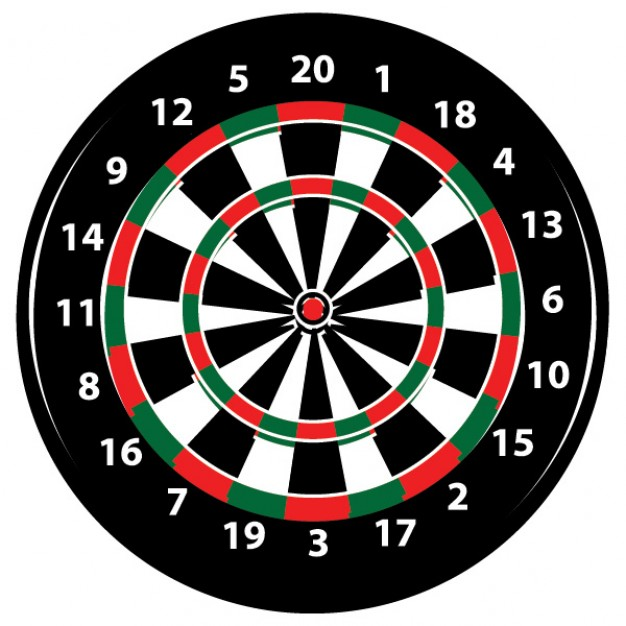
\includegraphics[width=0.5\textwidth]{darts}
\end{center}
\end{tcolorbox}
\paragraph{Вес} представленных гранат равен 0.5.
\paragraph{Дистанция} у гранат обычно Ближняя 5, Дальняя 20.
\paragraph{Центр Взрыва:} точка, из которой распространяется Взрыв.
\paragraph{Радиус Взрыва(РВ):} число метров, на которое распространяется Взрыв из центра Взрыва во все стороны. Если атака обладает свойством «Взрыв», то цель, против которой совершается проверка Доблести или Меткости, также считается находящейся в области Взрыва и получает Повреждения и прочие эффекты и от него тоже!
\paragraph{Сила Взрыва(СВ):} все существа, попавшие в радиус Взрыва, получают Пв, равные \textbf{|Сила Взрыва — БАЗщ — БДЗщ|}.
\paragraph{Газ:} газ распространяется в радиусе Взрыва и остается там какое-то время. Для определения длительности действия газа совершите проверку Неприятностей. Существа, вдохнувшие газ, страдают от эффектов яда, громко кашляют и чихают, если они еще в состоянии кашлять и чихать. Существа, имеющие Иммунитет к Ядовитым Пв, не подпадают под действие газа. В помещении увеличьте временные промежутки вдвое.
\trouble
{Штиль}%no sweat name
{Газ рассеивается чере 10 минут}%no sweat description
{Бриз}%tough day name
{Газ рассеивается через 5 минут}%tough day description
{Порыв ветра}%we have trouble name
{Газ рассеивается через 1 минуту}%we have trouble description
{Шторм}%fiasco name
{Газ рассеивается по истечении полного Круга}%fiasco description

\paragraph{Другие опасности Взрывов:} Взрывы опасны не только Повреждениями. Попавшие во Взрыв доспехи, щиты и прочие предметы, закрепленные на теле попавшего во Взрыв, получают \textbf{|Пв = Сила Взрыва — Прч|} и могут быть уничтожены. Если Взрыв достаточно силен, попавшие в него существа с воплями разлетаются в разные стороны! Если существо получает Повреждения от взрыва, его отбрасывает от центра Взрыва на \textbf{|Сила Взрыва — МСл отброшенного — МЛв отброшенного|} метров. Отброшенный получает столько Пв, сколько метров пролетел. Когда отброшенный сталкивается с другим существом, оно падает, если \textbf{|Сл отброшенного + БДЗщ отброшенного + БЩЗщ отброшенного $\pm$ БШР отброшенного| $\geq$ |Зщ существа + МСл существа $\pm$ Прч существа $\pm$ БШР существа|}. Существо получает 1 Пв за каждую единицу разницы не в свою пользу. В противном случае Пв получает отброшенный. Существо не может быть отброшено на большее число метров, чем получило Пв от Взрыва. Увеличьте расстояние броска в 2 раза за каждую категорию размера меньше Среднего и уменьшите в 2 раза за каждую категорию больше Среднего. Падения и столкновения наносят Дробящие Пв.
\newline
Если при подсчете дистанции отбрасывания получилось 0 или меньше, существо остается на месте.

\subsection{Спиок гранат}
\genAndGet{explosives}

\section{Защита}
\paragraph{Бонус к Защите (БЗщ):} доспехи и щиты дают Бонус к Защите. Герой не может надеть 2 комплекта доспехов одновременно, но может одновременно использовать 2 щита. В этом случае он получает БЗщ обоих щитов.
\paragraph{Класс Защиты(КЗ):} Добавляет свое значение к Размеру существа для определения условий Подавляющего превосходства, не меняя его размер для определения других условий.
\paragraph{Требуемая Выносливость(тВн):} Герой не может носить доспех или щит, если не обладает достаточной для этого Выносливостью. Сила не играет здесь важной роли — герой может поднять доспех и выдержать его вес, но выдохнется после нескольких минут активных действий. Разумеется, он может облачиться в тяжелый доспех, чтобы повыпендриваться перед девчонками или попозировать фотографу, но в бою представляет собой жалкое зрелище.
\newline
Если Выносливость героя меньше, чем тВн защиты, все физические проверки героя совершаются с Помехой, а все атаки по нему совершаются с Преимуществом.
\paragraph{ограничение модификатора Ловкости(оМЛв):} доспехи и щиты — тяжелые громоздкие конструкции, которые сильно ограничивают и сковывают движения. Некоторые доспехи и щиты ограничивают модификатор Ловкости, доступный герою для Защиты и проверок. Так, герой с 20 Лв (модификатор Лв +5), надевший кольчугу, будет добавлять к Защите и проверкам Ловкости и Навыков, основанных на Ловкости, лишь +3, потому что ограничение МЛв кольчуги составляет +3. Обратите внимание, что атаки любых видов основаны на Ловкости, так как модификатор Лв входит в состав Доблести и Меткости.
\paragraph{Количество помех для проверок Скрытности(ПС):} защита может шуметь при движении - звон сочленений, трение защитных пластин друг о друга, гул силовой установки в энергетических доспехах, это все мешает герою эффективно скрывать свое присутствие.
\paragraph{Надевание и снятие доспехов и щитов:} время, необходимое для этого, зависит от максимального модификатора Ловкости доспеха или щита. Если доспех или щит позволяет Любой модификатор Ловкости, время одевания и снятия составляет 1 минуту. Если максимальный модификатор Ловкости доспеха +2 или выше, время одевания составляет 5 минут, а время снятия составляет 1 минуту.
\newline
Если максимальный модификатор Ловкости +1 или ниже, время одевания составляет 10 минут (оно может быть сокращено до 5 минут, если кто-то помогает герою надевать доспех), а время снятия составляет 5 минут.
\paragraph{Шипы} на доспехе или щите позволяют эффективнее атаковать противника и охладить пыл любителей пообниматься. Шипы увеличивают параметр Выносливости, необходимой для ношения, на 1. Герой в шипованном доспехе, впечатанный в стену, может застрять в ней!
\paragraph{Единицы Здоровья} защиты равны \textbf{Вн}, необходимой для его ношения.
\paragraph{Прочность} защиты равна половине ее \textbf{ЕЗ}. Прочность вычитается из Единиц Здоровья, которые теряет защита.
\paragraph{Сопротивление к Повреждениям:} доспехи и щиты обладают Иммунитетом к Ядовитым Пв, Сопротивлением к Колющим, Проникающим, Огненным и Ледяным Пв и Уязвимы к Едким Пв.
\paragraph{Атаки по доспехам и щитам:} доспех или щит могут быть выбраны, как зона поражения (подробнее смотрите маневр «Сломать снаряжение» в разделе «Маневры»). Носитель получает Пв только в том случае, если доспех или щит получают Пв, которые не смогли поглотить их Прч и ЕЗ! Если доспех или щит уничтожены, носитель теряет их БЗщ, однако его МЛв все еще ограничен максМЛв доспеха или щита.
\paragraph{Удар щитом:} минимальная сила для ударов щитом равна минимальной Выносливости для ношения щита. Возможна ситуация, в которой герой может носить щит, но не может им бить.
\paragraph{Ширпотреб, индивидуальный заказ и шедевр:} дешевый, кое-как изготовленный доспех (вроде тех, в которых щеголяет уличная шпана) тяжел и неудобен. Выносливость, необходимая для его ношения, увеличивается на 1, а максимальный модификатор Ловкости понижается на 1. Если доспех не ограничивал модификатор Ловкости, то он получает максимальный модификатор в +4 и Осечку 5.
\newline
Доспех, изготовленный по индивидуальному заказы, безупречно подходит заказчику. Выносливость, необходимая для его ношения, уменьшается на 1, а максимальный модификатор Ловкости повышается на 1. Щиты в дополнение к этому повышают ЕЗ × 2 и Прочность × 2. Повысьте СП на 5.
\newline
Шедевр представляет собой безупречный экземпляр мастерской работы и получает все преимущества работы мастера. В дополнение, бонусы к Защите доспеха или щита возрастает на 1. Повысьте СП на 10.
\newline
Индивидуальный заказ и шедевр — штучные изделия. Все, кроме хозяина, при ношении получают эффекты ширпотреба, пока доспех не будет подогнан сведущим технарем под нового  ладельца.
\paragraph{Символ «*»} обозначает качества доспехов и щитов, не указанные в таблице и перечисленные в описательном блоке.
\paragraph{Символ «Ф»} обозначает доспехи, уместные лишь в фантастическом антураже.
\subsection{Броня}
\genAndGet{protection}{armor}

\subsection{Щиты}
\genAndGet{protection}{shields}


\subsection{Защита для больших и маленьких существ}
Повысьте СП доспеха или щита на 2 за каждую категорию размера больше Среднего. Стоимость доспехов и щитов для маленьких существ не меняется — меньшая стоимость материалов компенсируется сложностью работы. Увеличение СП за размер складывается с изменением СП за Халтуру, Работу мастера или Шедевр.
\paragraph{ЕЗ доспехов и щитов для больших и маленьких существ:} повысьте ЕЗ доспеха или щита в 1.5 раза за каждую категорию размера больше Среднего и понизьте в 1.5 раза за каждую категорию размера меньше Среднего. Например, латы для Среднего человека имеют 15 ЕЗ и Прч 7. Латы для Маленького полурослика будут иметь 10 ЕЗ и Прч 5, а латы для Большого огра — 22 ЕЗ и Прч 11!
\section{Медикаменты и яды}
\paragraph{Интоксикация.} Ядовитые повреждения считаются отдельно от остальных повреждений и отражают то, насколько много яда попало в организм и сколько еще он может сопротивляться яду.
\newline
Значение Интоксикации героя может быть больше, чем его максимальные ЕЗ.
\newline
Если значение Интоксикации превышает текущие ЕЗ героя, он становится Отравлен и на него накладываются эффекты Интоксикации \textit{всех} ядов, которые наносили ему Ядовитые повреждения. Для того, чтобы снять состояние Отравления, герой должен восстановить ЕЗ до уровня, когда значение Интоксикации становится меньше, чем текущие ЕЗ героя.
\newline
Во время отдыха герой понижает Интоксикацию на столько, сколько восстанавливает ЕЗ. Но если он применяет стимулятор или зелье, то он не снимает Интоксикацию, если это не указано в их описании. Так же если герой обращается за помощью к целителю, то Интоксикация снимаются отдельно.
\newline
Например, если у героя Иноксикация равна 5 и он получил 6 повреждений из других источников, Доку нужно потратить 11 зарядов своего Атрибута, чтобы полностью исцелить героя.
\paragraph{Первичный эффект:} Разовый эффект Лекарства или Яда. Для сопротивления эффекту герой должен преуспеть в проверки Вн против \textbf{|10+Токсичность|}.
\paragraph{Эффект Интоксикации:} целебные зелья, таинственные эликсиры и мощные стимуляторы зачастую являются не очень-то и полезными при частом применении. Каждое применение препаратов наносит при потреблении Ядовитые повреждения. Побочный эффект прекращается, как только Интоксикация становится меньше, чем его текущие ЕЗ.
\paragraph{Токсичность:} количество Ядовитых повреждений, которое наносит препарат при применении.
\paragraph{Отравленное оружие:} Если в названии яда есть свойство [масло], его можно нанести на оружие.
\newline При нанесении масла на оружие, он действует в течение \textbf{Тк} атак. Это правило действует как на оружие ближнего боя, так и на дальнобойное оружие. Для дальнобойного оружия это значит, что порция масла была распределена равномерно между боеприпасами. Если атака нанесла хотя бы 1 Пв, цель дополнительно получает Ядовитые повреждения в размере Токсичности Яда и должен сопротивляться его Первичному эффекту.
\paragraph{КУ Ядовитых повреждений.} Если атака, наносящая Ядовитые повреждения наносит критический удар, то тот яд, которым наносится атака сразу вызывает Эффект Интоксикации и не прекратит свое действие, пока с героя не будут сняты \textit{все} Ядовитые повреждения.

\subsection{Медикаменты}
\genAndGet{drugs}{meds}
\subsection{Яды}
\tbd
\section{Инструменты Могущества \tbd}
В этом разделе описаны могущественные артефакты, высокотехнологичные прототипы и технологические чудеса, которые позволяют герою достичь и преодолеть предел своих возможностей. Обычно Инструменты Могущества встречаются только в фантастическом антураже.

\paragraph{Название} Инструмента отражает его дух, историю или возможности. Редко названия Инструментов бывают обыденными.
\paragraph{Базовый предмет} Зачастую Инструмент построен на основе уже существующего, а иногда и весьма распространенного в мире, предмета, оружия или элемента экипировки. Обычно Инструмент сохраняет все характеристики Базового предмета и лишь усиливает их своими способностями.
\paragraph{Запас Энергии: }иногда у Инструмента есть собственный запас Энергии, который можно тратить на активацию его Могуществ. Способ восстановления этой энергии может сильно отличаться в зависимости от антуража. Если у Инструмента нет запаса Энергии, то для его активации используется Энергия владельца.
\paragraph{Сложность Приобретения(СП): }некоторые Инструменты научились довольно ловко воспроизводить и их даже можно увидеть на полках магазинов! Но если в описании нет СП, то Инструмент нельзя просто купить. Придется искать его в древних руинах, секретных лабораториях, а иногда и выпрашивать у богов.
\paragraph{Описание }Инструмента говорит о его виде и о нарративе его использования. Механика его работы описана в Трюках, Могуществах и Ходах Инструмента.
\paragraph{Трюки }Инструмента - это его свойства, которые герой может использовать когда захочет или же они работают постоянно.
\paragraph{Могущества }Инструмента требуют Энергии для активации. В описании каждого Могущества Инструмента обязательно указана его \textbf{Стоимость}.
\paragraph{Ходы }Инструмента позволяют совершать невозможное, но требуют за это обрыв Нитей героя. В описании каждого Хода Инструмента обязательно указана его \textbf{Стоимость}.

\genAndGet{powerTools}

\section{Импланты}
Импланты - это подвид Инструментов могущества, который имеет некоторые особенности:
\begin{itemize}
\item Имплант нельзя просто снять или надеть - для этого требуется помощь специалиста, и порой очень дорогостоящая.
\item Имплант всегда имеет прямой доступ к Энергии владельца - ее можно тратить на активацию его Могуществ без ограничений, однако использовать для этого внешнюю батарею нет никакой возможности.
\item Имплант найти гораздо легче, чем другие Инструменты Могущества - у них почти всегда есть СП.
\end{itemize}

\genAndGet{powerTools}{implants}
\section{Транспорт}
В этом разделе описаны механизмы и живые существа, которых можно использовать, как транспорт
\newline Символ «Ф» обозначает вид транспорта, уместный лишь в фантастическом антураже.
\newline Если в столбце размера указана литера \textbf{Ж}, то этот вид транспорта является животным.
\paragraph{Ограничение Модификатора Ловкости(оМЛв):} Крупные транспортные средства ворочаются неохотно, а разогнавшись, не спешат тормозить оМЛв определяет максимальны МЛв, который водитель может добавить к проверкам Эксплуатации при управлении транспортным средством.
\paragraph{Ограничение Модификатора Ловкости(оМЛв) для животных:} Не вся животина резво подчиняется командам погонщика или наездника. Максимальный МЛв, который может герой добавить к проверкам Общения с животными равен МЛв самого животного.
\paragraph{Проходимость транспортного средства(П):} транспорт не может передвигаться по местности с Опасностью, превышающей его Проходимость. Проходимость животных увеличивается на 1, если они не несут груза или всадников.
\begin{itemize}
\item литерой \textbf{Л} обозначена способность транспорта к полетам. Проходимость летающих транспортных средств учитывается только при взлете и посадке. Также они всегда могут передвигаться на пределе скорости, если возникла такая необходимость.
\item литерой \textbf{В} обозначено то, что транспорт может перемещаться только по воде.
\item литерой \textbf{К} обозначена способность транспорта к совершению межпланетных и межзвездных путешествий. \tbd(описать, что скорость межпланетного перемещения определяется сеттингом, а скорость в таблице определяет скорость при околопланетном маневрировании)
\end{itemize}
\paragraph{Защита транспортного средства:} предполагается, что транспортные средства из этой уже оснащены всеми возможными защитными приспособлениями в пределах разумной целесообразности. Модификатор Ловкости водителя прибавляется (или отнимается, если он отрицательный) к Защите ТС.
\paragraph{Перегруженный транспорт:} если нагрузка транспортного средства превышает Грузоподъемность не более чем в 2 раза, водитель получает Помеху на проверки Эксплуатации. Если нагрузка транспортного средства превышает Грузоподъемность не более чем в 3 раза, водитель получает 2 Помехи на Эксплуатацию.
\paragraph{Буксировка:} предполагается, что транспортное средство может буксировать вес, не превышающий свой собственный. Если буксируемый вес превышает вес транспортного средства не более чем в 2 раза, водитель получает Помеху на Эксплуатацию. Если буксируемый вес превышает вес транспортного средства не более чем в 3 раза, водитель получает 2 Помехи на Эксплуатацию.
\paragraph{Маневренность.} Во многих ситуациях важны не только проходимость и скорость автомобиля, но и его способность избегать препятствий. Маневренность транспорта равна \textbf{|Проходимость — Модификатор размера транспортного средства|}.Маневренность добавляется к навыку
водителя (или отнимается, если она отрицательная) при проверке Эксплуатации для совершения сложных поворотов и перестроений.
\paragraph{Ховер:} в научно-фантастических сеттингах транспортное средство может быть оснащено ховер-левитатором. Его СП возрастает на 5, его Проходимость возрастает до 5.
\paragraph{Потеря ЕЗ транспортным средством:} после потери \textbf{1/3 ЕЗ}
транспортное средство теряет половину своей Скорости. После
потери \textbf{2/3 ЕЗ} проверки Эксплуатации совершаются с Помехой.
\newline
Если транспортное средство одномоментно теряет \textbf{1/4 или более своих ЕЗ}, водитель должен совершить проверку Эксплуатации против 15. При провале транспортное средство глохнет.
\newline
Попадания по двигателю или ходовой части транспортного средства могут быть весьма опасны! Если зона поражения одномоментно теряет \textbf{1/5 или более от максимальных Единиц Здоровья}, она выходит из строя. Лишние Повреждения теряются, но водитель должен совершить проверку Эксплуатации против 15. При провале транспортное средство глохнет.
\newline{Ремонт транспортного средства:} восстановление каждых 5 ЕЗ требует 1 часа работы, наличия Ремонта у механика и имеет СП 1.

\paragraph{Cкорость(Ск)} Скорость трансопорта во время путешествий(в км/ч). Численно она равна Ск транспорта во время Боевых Сцен и она \textbf{значительно ниже} максимальной скорости, которую можно выжать из этого транспорта. Если у транспорта в этой графе присутствует литера М, это значит, что его обычная скорость равна максимальной и этот транспорт не может двигаться \textbf{Маршем}(если только скорость самого медленного члена каравана не в два раза меньше, чем скорость этого транспорта).
\paragraph{Расход топлива(Р)} определяет сколько Зарядов Топлива(или килограмм фуража для животных) тратит тот или иной вид транспорта не каждые 10 км пути.
\paragraph{Грузоподъемность/Вес(ГВ)} определяет количество полезной нагрузки(за исключением полных баков топлива), которую может вести транспорт без перегрузки и вес самого транспорта для определения возможностей буксировки.

\subsection{Описание транспорта}
\genAndGet{transport}{transport}
\endinput
\begin{center}
\begin{longtable}{|p{2.5cm}||c|c|c|c||c|c|c||c|c|c|}
\hline
Название & 
Размер & Зщ & Прч & ЕЗ & 
оМЛв & П & Ск & 
ГВ & Р & СП \\ \hline \hline

Велосипед & 
М & 10 & 1 & 15 & 
- & 4 & СЛ+ВН водителя & 
80/15 & - & 7 \\ \hline

Мотоблок & 
М & 10 & 2 & 15 & 
+3 & 8М & 5* & 
500/50 & 6 & 10 \\ \hline

Мотороллер & 
М & 11 & 2 & 25 & 
- & 3 & 30 & 
100/100 & 3 & 10 \\ \hline

Мопед & 
М & 10 & 1 & 20 & 
- & 4 & 40 & 
100/100 & 3 & 10 \\ \hline

Скутер & 
С & 13 & 2 & 40 & 
+5 & 3 & 60 & 
150/300 & 6 & 12 \\ \hline

Мотоцикл & 
С & 12 & 3 & 40 & 
+5 & 3 & 90 & 
150/300 & 6 & 12 \\ \hline

Мусорный багги & 
Б & 14 & 3 & 50 & 
+4 & 4 & 80 & 
350/750 & 12 & 15 \\ \hline

Малолитражка & 
Б & 13 & 4 & 55 & 
+3 & 2 & 70 & 
420/750 & 9 & 15 \\ \hline

Легковой автомобиль & 
О & 14 & 4 & 60 & 
+3 & 2 & 100 & 
500/1300 & 15 & 20 \\ \hline

Прокачанная тачка & 
О & 13 & 5 & 70 & 
+2 & 2 & 130 & 
420/1800 & 30 & 25 \\ \hline

Спорткар & 
О & 12 & 4 & 65 & 
+4 & 1 & 150 & 
300/1400 & 36 & 25 \\ \hline

Лимузин & 
О & 13 & 7 & 80 & 
+1 & 1 & 100 & 
700/200 & 21 & 20 \\ \hline

Минивэн & 
О & 13 & 5 & 75 & 
+2 & 2 & 80 & 
1000/2000 & 18 & 25 \\ \hline

Джип & 
Б & 14 & 5 & 60 & 
+3 & 3 & 90 & 
550/1700 & 24 & 25 \\ \hline

Арммейский джип & 
О & 14 & 10 & 80 & 
+1 & 4 & 60 & 
1000/2900 & 33 & 30 \\ \hline

Пикап & 
О & 13 & 7 & 70 & 
+2 & 3 & 80 & 
720/2100 & 30 & 25 \\ \hline

Автобус & 
Г & 13 & 7 & 100 & 
+1 & 3 & 50 & 
9500/6000 & 30 & 30 \\ \hline

Грузовик & 
Г & 15 & 10 & 90 & 
+1 & 3 & 50 & 
9000/8000 & 45 & 30 \\ \hline

Армейский грузовик & 
Г & 15 & 13 & 100 & 
+1 & 4 & 50 & 
8000/8000 & 45 & 33 \\ \hline

Тягач & 
Г & 14 & 10 & 110 & 
+1 & 3 & 80 & 
8000/15000* & 45 & 35 \\ \hline

Армейский тягач & 
Г & 14 & 15 & 120 & 
+1 & 4 & 80 & 
10000/34000* & 60 & 38 \\ \hline

Трактор & 
Г & 14 & 10 & 90 & 
+1 & 4 & 20 & 
3500/3500 & 30 & 30 \\ \hline

Бульдозер & 
Г & 12 & 13 & 120 & 
0 & 3 & 8 & 
4000/18000 & 36 & 30 \\ \hline

БМП & 
Г & 17 & 15 & 130 & 
0 & 4 & 40 & 
9000/13000 & 45 & 40 \\ \hline

Танк & 
Г & 17 & 20 & 130 & 
0 & 4 & 30 & 
10000/45000 & 60 & 50 \\ \hline

Легкий винтовой самолет & 
Г & 14 & 5 & 60 & 
- & 1** & 160 & 
400/750 & 45 & 35 \\ \hline

Грузовой винтовой самолет & 
Г & 13 & 12 & 120 & 
0 & 1** & 300 & 
60000/120000 & 90 & 70 \\ \hline

Военный вертолет & 
Г & 17 & 7 & 80 & 
+4 & 4** & 200 & 
5000/7000 & 60 & 50 \\ \hline

\end{longtable}
\end{center}




*Через черту указана максимальная грузоподъемность полуприцепа, который может перевозить тягач.
**

\chapter{БОЕВЫЕ СТОЛКНОВЕНИЯ}
\paragraph{}
Эта часть полностью посвящена сражениям и их последствиям.
Здесь рассказывается о действиях, доступным героям в бою
и о ранах, которые герои могут нанести и получить.
\section{Тип Повреждений}
в зависимости от типа, повреждения могут иметь разные эффекты КУ и могут быть увеличены или уменьшены в зависимости от того, какие есть сопротивления или уязвимости у цели. Атаки имеют один из следующих типов Повреждений:
\newline
\textbf{(Д)}робящие, \textbf{(Е)}дкие, \textbf{(К)}олющие, \textbf{(Л)}едяные, \textbf{(О)}гненные, \textbf{(П)}роникающие, \textbf{(Р)}убящие, \textbf{(Э)}лектрические, \textbf{(Я)}довитые.
\newline
Хотя задача большинства атак — понижение ЕЗ цели, достигается она по-разному. Пытаться повредить рапирой каменную стену — не самая здравая идея, здесь лучше сработают молот или хотя бы дубина. Зато меткий укол в глаз способен не только ослепить противника, но уложить его на месте!
\paragraph{Уязвимость, Сопротивление, Иммунитет и Родная стихия:} Уязвимость к определенному типу Пв увеличивает успешно нанесенный урон в 2 раза. Сопротивление к определенному типу Пв уменьшает успешно нанесенный урон в 2 раза. Иммунитет к определенному типу Пв делает существо абсолютно невосприимчивым к этому типу Пв. Тип Пв, являющийся для цели Родной стихией, не отнимает ее ЕЗ, а восстанавливает их на то число, которое цель потеряла бы, не имея Родной стихии. ЕЗ цели все еще не могут превышать максимальной величины.
\paragraph{Атаки с несколькими типами Повреждений:} некоторые виды оружия могут наносить Пв разных типов — например, меч может наносить как Рубящие, так и Колющие Пв. В этом случае выберите тип Пв перед атакой.
\newline
Также существуют виды оружия, которые имеют несколько типов Повреждений одновременно — например, удар горящим факелом нанесет Огненные и Дробящие Пв. Возможна ситуация, в которой цель будет иметь Уязвимость к нескольким типам Пв атаки одновременно или даже Уязвимость к одному из них и Сопротивление к другому.
\newline
Если цель имеет Уязвимость к нескольким типам Пв атаки сразу, удвойте успешно нанесенные Пв за каждую Уязвимость. Например, если гигантский слизень имеет Уязвимость к Огненным Пв и Дробящим Пв, то удар горящим факелом нанесет в 4 раза больше Пв, чем обычно.
\newline
Уязвимость и Сопротивление компенсируют друг друга. Например, если цель имеет Сопротивление к Огненным повреждениям и уязвимость к Дробящим, то атака факелом будет наносить обычное количество повреждений по цели.
\newline
Иммунитет к любому типу Пв, которые включает атака, не позволяет ей наносить Повреждения цели.
\paragraph{Эффекты КУ} от разных типов повреждений:
\begin{itemize}
\item[--] \textbf{Дробящие:} получивший КУ Оглушен.
\item[--] \textbf{Едкиe:} получивший КУ начинает Растворяться. Состояние наступает даже в том случае, если цель не получила Пв при атаке.
\item[--] \textbf{Колющие:} получивший КУ страдает от Внутреннего кровотечения.
\item[--] \textbf{Ледяные:} получивший КУ становится Неподвижным до конца своей следующей Очереди.
\item[--] \textbf{Огненные:} получивший КУ Загорается.
\item[--] \textbf{Проникающие:} снаряд засел внутри тела! Получивший КУ страдает от Внутреннего кровотечения. После завершения боя он страдает от Агонии до тех пор, пока снаряд не будет извлечен (Врачевание против 15).
\newline
Если герой подвергается магическому лечению до того, как снаряд извлечен, он больше не страдает от Агонии и Внутреннего кровотечения, но боль дает о себе знать. Все активные проверки героя совершаются с Помехой до тех пор, пока снаряд не извлечен. Последующая сложность проверки Врачевания для извлечения снаряда возрастает до 20.
\item[--] \textbf{Рубящие:} получивший КУ страдает от Кровотечения.
\item[--] \textbf{Электрические:} получивший КУ сбит с ног.
\item[--] \textbf{Ядовитые:} на получившего КУ накладывается эффект яда.
\end{itemize}
\section{Состояния}
Физические  воздействия могут повлиять на состояние (и поведение) героя, как в бою, так и вне его. Эффекты двух
одинаковых состояний, происходящих из различных источников, не складываются, за исключением Внутреннего Кровотечения, Возгорания, Кровотечения, Отравления и Растворения. Эффекты различных состояний воздействуют на героя одновременно.
\paragraph{Агония:} герой охвачен мучительной болью. Герой может действовать только в случае успешной проверки Вл против 20. В боевых сценах совершайте проверку каждую Очередь героя, в остальных — один раз за сцену. При провале все, на что способен герой — лежать, вопить и поносить свою злую Судьбу. При успехе проверки герой держит себя в руках, но не может совершать Маневры и передвигается с половинной Ск. Состояние длится, пока герой не будет исцелен чарами (если Агония вызвана потерей ЕЗ), не получит квалифицированную врачебную помощь (если Агония вызвана Переломом) или сильное обезболивающее.
\paragraph{Внутреннее кровотечение:} жизненно важные органы героя повреждены. Каждую свою Очередь герой теряет |5 — МВн| ЕЗ (минимум 2 ЕЗ) до тех пор, пока не будет исцелен чарами или не получит квалифицированную врачебную помощь (Врачевание против 15).
\paragraph{Возгорание:} в начале своей Очереди горящее существо или предмет теряет 5 ЕЗ. Горящее существо может пропустить свою Очередь, чтобы потушиться. В этом случае до начала следующей Очереди существа атаки по нему совершаются по правилам Внезапного нападения. Состояние длится \textbf{|5 — МЛв цели|} Кругов (минимум 1 Круг).
\paragraph{Кровотечение:} герой истекает кровью. Каждую свою Очередь герой теряет число ЕЗ, равное БПв оружия, вызвавшего КУ(мин 1). Состояние длится до тех пор, пока герой не будет исцелен или перевязан (Врачевание против 10).
\paragraph{Неподвижность:} по каким-то причинам герой не может двигаться и защищать себя. Он может быть схвачен, заморожен, опутан сетью или просто спит. Герой теряет бонуз защиты щита и бонус ловкости к защите. Все атаки по герою совершаются с Преимуществом.
\paragraph{Оглушение:} герой ненадолго теряет связь с реальностью (обычно из-за доброго удара по голове или под дых). Герой не может совершать Действие в свою следующую Очередь. В дальнейшем герой совершает все свои активные проверки с Помехой число Очередей, равное \textbf{|5 — МВн|} (минимум 1 Очередь).
\paragraph{Ослепление:} герой ничего не видит. Все атаки по нему совершаются по правилам Внезапного нападения. Герой атакует с 2 Помехами. Он не может атаковать цели, находящиеся от него на расстоянии (в метрах) большем, чем его Наблюдательность.
\paragraph{Отравление:} герой находится под действием яда. Смотрите описание яда для определения эффекта.
\paragraph{Ошеломление:} герой приходит в замешательство и не может совершать Действие в свою следующую Очередь. В дальнейшем герой совершает все свои активные проверки с Помехой число Очередей, равное \paragraph{|5 — МИн|} (минимум 1 Очередь). Также это состояние может быть причиной недосыпа, злоупотребления алкоголем или наркотическими зельями. Тогда избавиться от него поможет только полноценный отдых.
\paragraph{Ранен:} если ЕЗ героя достигают 2/3 от максимальных, то он Ранен. Его Ск ополовинивается. Обычно это состояние связано с потерей ЕЗ героем, но иногда оно возможно и в иных случаях — например, если герой страдает от вывиха или последствий болевого приема.
\paragraph{Растворение:} в начале своей Очереди существо или предмет получает 1 Пв вне зависимости от своей Прч. Если жертва была одета, она может остановить действие эффекта, пропустив 1 Очередь и сорвав с себя одежду, хотя снятие доспеха может занять куда больше времени! Если же одежды на жертве не было… Ей понадобится помощь квалифицированного медика и проверка Медицины против 15. Растворение вызывается множеством самых различных субстанций и веществ, поэтому способ нейтрализации, который сработал в прошлый раз, в следующий может сделать только хуже! Проверка Медицины необходима для каждого нового источника Растворения.
\newline
Если меры не были приняты, состояние заканчивается через \textbf{|10 + Пв, нанесенные вызвавшей состояние атакой|} Кругов. В конце сцены совершите проверку Неприятностей, чтобы узнать, пришло ли в негодность снаряжение жертвы (при желании можно совершить отдельную проверку для каждого предмета).
\trouble
{Отдушка}%no sweat name
{Никаких последствий, кроме специфического запаха, который исчезнет после хорошей стирки}%no sweat description
{Патина}%tough day name
{Незначительные повреждения. Герой может исправить их самостоятельно, совершив проверку соответствующего НавыкаЭ против 15 или заплатив ремесленнику 1/4 СП предмета (минимум 1 СП). До завершения ремонта предмет получает Осечку 6.}%tough day description
{Ржа}%we have trouble name
{Серьезные повреждения, все еще поддающиеся ремонту.Герой может исправить их самостоятельно, совершив проверку Ремонта против 20 или заплатив ремесленнику 1/2 СП предмета (минимум 1 СП). До завершения ремонта предмет получает Осечку 10.}%we have trouble description
{Труха}%fiasco name
{Снаряжение приведено в полнейшую негодность. Возможно, удастся всучить его подвыпившему старьевщику и выручить пару медяков.}%fiasco description
\paragraph{Серьезно ранен:} если ЕЗ героя достигают 1/3 от максимальных, то он Серьезно ранен. Все его активные проверки совершаются с Помехой. Обычно это состояние связано с потерей ЕЗ героем, но иногда оно возможно и в иных случаях — например, если герой страдает от вывиха или последствий болевого приема.
\paragraph{Сон:} герой спит. Все проверки Наблюдательности героя совершаются с Помехой. Пока герой спит, он Неподвижен. Если герой проснулся и вынужден сразу же действовать, он Ошеломлен. Героя автоматически разбудит достаточно громкий звук — выстрел из пистолета или звон медного колокольчика. Более тихие звуки потребуют проверки Наблюдательности (с Помехой)!
\paragraph{Удушье:} герой задыхается. Все его проверки совершаются с Помехой. Герой Потеряет сознание, если состояние продлится дольше, чем \textbf{|Вн × 10|} секунд, и умрет вне зависимости от величины его ЕЗ, если состояние продлится дольше, чем \textbf{|Вн × 20|} секунд.
\paragraph{Ужас:} герой дрожит от ужаса. Он совершает все активные проверки с Помехой, пока источник его ужаса находится поблизости (в зоне видимости или слышимости). В дальнейшем состояние длится число Очередей, равное \textbf{|10 — Вл героя|}.
\paragraph{Усталость:} все активные проверки совершаются героем с Помехой. Атаки по герою совершаются с Преимуществом.
\section{Подавляющее Превосходство и Внезапная Смерть}
Если разница в размере существ составляет 3 категории или больше, у большего существа есть Подавляющее Превосходство над меньшим. Любая успешная атака существа с Подавляющим Превосходством грозит Внезапной Смертью меньшему существу, одновременно с этим любая атака меньшего существа настолько незначительна, что не может нанести повреждений большему даже при Критическом Ударе. Так же меньшее существо не может наложить эффектов КУ на большее существо с Подавляющем превосходством.
\paragraph{Класс Защиты и Повреждений.} Некоторые виды вооружений и защиты созданы специально для того, чтобы бороться с крупными противниками и защищаться от них. Существо и его атаки можгут считаться большего или меньшего размера, для определения условий Подавляющего превосходства, если снаряжение, которое оно использует имеет Класс Защиты или Класс Повреждений.

\paragraph{Внезапная Смерть.} Иногда урон, который предстоит получить герою или статисту настолько велик, что никакая защита его не спасет, только чудо. Статисты умирают сразу(если судьба героев не вступится за них), герои и персоны совершают проверку Неприятностей.
\trouble
{Ни царапины}%no sweat name
{Герой чудом пережил прямое попадание. Хотя постойте - она мимо прошла!}%no sweat description
{Задело}%tough day name
{Героя зацепило осколками и ударной волной. Он теряет половину текущих ЕЗ и должен совершить проверку Опасной раны, даже если потерял меньше 1\\4 максимальных ЕЗ.}%tough day description
{Потрепало}%we have trouble name
{Героя приложило крупным осколком. Его ЕЗ становятся равными 0 и он теряет сознание.}%we have trouble description
{Уничтожило}%fiasco name
{От героя осталось только воспоминание. Даже чудотворец не сможет вернуть его к жизни.}%fiasco description
\section{Раны и их последствия}
\paragraph{}
Единицы Характеристик (ЕХ) и их потеря: некоторые атаки — как правило, яды, отнимают не ЕЗ жертвы, а понижают ее Характеристики. Например, ядовитая паучья слюна понижает Ловкость жертвы на 2. Под потерей ЕХ понимаются все подобные случаи.
\newline
Если герой пережил Повреждения, Единицы Здоровья и Единицы Характеристик могут быть восстановлены до максимума посредством отдыха или медицинской помощи. О восстановлении ЕЗ и ЕХ подробнее читайте в разделе «Отдых».
\paragraph{Опасная рана:} если герой одномоментно теряет 1/4 и более от максимальных ЕЗ, он должен совершить проверку Вн против 15. Если герой проходит проверку, то он продолжает сражаться. В противном случае он Теряет сознание.
\paragraph{Болевой шок:} если в течение Круга герой одномоментно теряет число ЕЗ, превышающее его \textbf{|Вл|}, то следующая активная проверка героя совершается с Помехой. Разумеется, это относится к живым существам, которые в принципе способны испытывать боль.
\paragraph{Потеря сознания:} герой, потерявший сознание, придет в себя через \textbf{|10 минут × потерянные ЕЗ|}. Если не замерзнет, не истечет кровью, не будет добит победителями или съеден дикими тварями. Герой, пришедший в сознание в 0 ЕЗ, страдает от ран и находится в Агонии!
\newline
Герой немедленно приходит в сознание, если его ЕЗ поднимаются на 1 или больше.
\paragraph{Смерть:} как только герой теряет последнюю ЕЗ, он должен совершить проверку Вн против 15. Если герой проходит проверку, то Теряет сознание и остается жив (и обзаводится парой впечатляющих шрамов). В противном случае герой умирает.
\paragraph{Смерть и статисты:} для ускорения боевых сцен мастер может считать проверки Выносливости статистов при Потере конечностей, Опасных ранах и Смерти автоматически проваленными и совершать их только в тех сценах, которые он и игроки считают важными. Также мастер может делать проверки, если игроки желают захватить статиста живым.
\subsection{Тяжелые травмы}
\paragraph{Однорукие герои:} однорукие герои не могут использовать Двуручное оружие. Если рука обрублена ниже локтя, герой может закрепить на ней щит или одноручное оружие.
\paragraph{Одноногие герои:} одноногий герой с костылем или протезом считается перемещающимся по Трудному ландшафту. Да, это значит, что одноногий герой с костылем или протезом и Чувством равновесия не испытывает никаких неудобств при движении. Костыль может использоваться для атаки! Без костыля или протеза одноногий герой перемещается на 1/3 своей Ск. Одноногие герои не могут использовать Громоздкое оружие.
\paragraph{Безногие герои:} безногие герои понижают свой размер на 1 категорию. Ск безногих героев составляет 1. Если у безногого героя есть какое-то средство перемещения — например, тачка с колесиками — при помощи Перемещения он может двигаться на число метров, равное своему МЛв (минимум на 2 метра). Безногий герой атакует в ближнем бою с Помехой. В ближнем бою враги атакуют безногого героя с Преимуществом. Безногие герои не могут использовать Громоздкое и Длинное оружие.
\paragraph{Потеря глаз:} герой, лишившийся двух глаз, перманентно находится в состоянии Ослепления. Одноглазый герой совершает проверки Меткости с Помехой.
\section{Боевые сцены}
Боевая сцена начинается, если один или несколько героев подверглись атаке, либо напали на кого-то сами. В начале боевой сцены:
\begin{enumerate}
\item Определите, подвергся ли кто-то из участников Внезапному нападению. Обычно это сопряжено с проваленными проверками Наблюдательности против Скрытности противника. Если никто из участников сражения не пытался передвигаться скрытно и ожидал нападения, фактор внезапности вряд ли стоит учитывать. С другой стороны, Стремительный герой, герой с трюком «Гопля!» или герой с высокой Реакцией вполне может застать противников врасплох, молниеносно выхватив оружие и атаковав!
\item Определите позиции участников сцены относительно друг друга и окружающих предметов. На обсуждение этого стоит потратить несколько минут (или даже больше), чтобы игроки четко представляли возможности героев и их противников.
\item Начало Круга. Все участники сцены действуют в порядке, определяемом их Реакцией. Возможно, для завершения битвы понадобится больше одного Круга.
\end{enumerate}
\paragraph{Круг:} в бою герои и статисты действуют по Очереди. Один полный \textbf{Круг} (то есть Очереди всех героев и статистов, принимающих участие в сцене) занимает \textbf{5 секунд}. Подразумевается, что герои и статисты действуют в бою одновременно, однако для удобства игры круг разделен на Очереди. Статисты под управлением мастера действуют в одну общую Очередь, однако мастер может разделить их Очереди в соответствии с параметрами Реакции. Общая Очередь ориентируется на статиста с наименьшей Реакцией.
\paragraph{Очередность в бою:} первым действует герой или статист с наибольшей Реакцией. Если у двух героев или статистов одинаковая Реакция, первым действует тот, у кого больше Ловкость. Если и они равны, первым действует выигравший Состязание в Реакции.
\paragraph{Очередь:} Очередь героя состоит из Перемещения, Действия и Быстрого действия. В течение своей Очереди герой может:
\begin{itemize}
\item[--] \textbf{Совершить Перемещение.} Для Перемещения используется значение Ск — столько метров/клеток может преодолеть герой. Герой может отказаться от Перемещения, чтобы получить дополнительное Быстрое действие.
\item[--] \textbf{Совершить Действие.} Во время Действия герой использует предметы, атакует, творит чары, убеждает окружающих прекратить кровопролитие или делает что-то еще, требующее концентрации внимания.
\item[--] \textbf{Совершить Быстрое действие.} Быстрое действие включает односложные фразы, быстрые жесты, шаги в пределах 1 метра и броски предметов без намерения кому-то повредить или поразить конкретную цель. Хрупкие предметы могут сломаться или разбиться! У героя есть лишь одно Быстрое действие за круг, но мастер может отступать от правила, если считает ситуацию располагающей к этому. Иногда выполнение Быстрого действия возможно и в чужую Очередь. Такие случаи указаны в описании соответствующих Трюков или Атрибутов.
\end{itemize}
\begin{tcolorbox}
Герой может отказатьсяот Действия, чтобы совершить дополнительное Перемещение или дополнительное Быстрое действие.
\newline
Так же герой может отказаться от Перемещения, чтобы совершить дополнительное Быстрое действие.
\end{tcolorbox}
Герой может отказаться от Перемещения или Действия, чтобы подняться с земли, или взять предмет, или аккуратно положить предмет, или привести оружие в боевую готовность, или убрать оружие в ножны, или перезарядить оружие со свойством «Перезарядка», или вскочить в седло.
\newline
Перемещение, Действие и Быстрое действие используются в любых комбинациях. Например, совершая Быструю атаку, герой со Скоростью 6 может за одну Очередь пройти на 1, атаковать, потом пройти на 2, атаковать еще раз, затем пройти на 3 и уронить предмет.
\subsection{Детали боевой сцены}
\paragraph{Внезапное нападение.} Если герой не заметил врага или заметил в последний момент (то есть провалил проверку Наблюдательности против Скрытности врага), он захвачен врасплох. Герой не может Перемещаться и Действовать независимо от своей Реакции, а также вычитает МЛв и БЩЗщ из своей Зщ. Если герой дожил до своей следующей Очереди, он сражается по обычным правилам.
\paragraph{Все на одного:} сражение с несколькими противниками требует от воина высочайшего мастерства. Если герой сражается с несколькими противниками, в начале Очереди он должен выбрать, кому из них он уделяет больше внимания. Выберите число противников, равное \textbf{|1 + ММд героя|} (минимум 1). Они атакуют героя, как обычно. Все противники сверх этого числа атакуют героя с Преимуществом.
\paragraph{Ложись!:} герой может упасть, использовав Быстрое действие. Дистанционные атаки по лежащему герою совершаются с Помехой, атаки в ближнем бою по нему совершаются с Преимуществом. Лежащий герой может ползти с 1/2 Ск и атаковать в ближнем бою с Помехой. В остальном герой действует по обычным правилам.
\paragraph{Невидимки:} если герой атакует невидимого (из-за чар, укрытия или по иным причинам) противника, бросок совершается с Помехой. Если невидимого противника нет в атакуемой области, герой автоматически промахивается. Невидимые существа атакуют по правилам Внезапного нападения. Если существо невидимо благодаря Скрытности, а не волшебству, то, атаковав, оно обнаружит себя вне зависимости от успеха атаки.
\paragraph{Перемещение через занятые области:} если герой желает пройти через область, занятую враждебным существом, он должен пройти проверку Атлетики против \textbf{|10 + Дб противника $\pm$ БШР противника|}. В случае успеха герой передвигается через занятую область, в случае провала падает рядом с противником. Перемещение героя на этом заканчивается.
\paragraph{Трудный ландшафт.} Иногда перемещение героя затруднено густым подлеском, глубоким снегом, скользким льдом, качающейся палубой. В такой ситуации Ск героя ополовинивается.
\subsection{Зоны поражения}
Герой может выбрать для атаки любую из перечисленных зон. Если при атаке не заявлена специфическая Зона поражения, удар наносится в торс.
\begin{center}
\begin{tabular}{|c|c|}
\hline
Зона поражения & Штраф к Доблести/Меткости \\ \hline
Торс & 0 \\ \hline
Конечность & -2 \\ \hline
Пах & -3 \\ \hline
Шея & -5 \\ \hline
Голова & -5 \\ \hline
Глаз & -7 \\ \hline
\end{tabular}
\end{center}
\paragraph{Торс:} попадание по торсу не вызывает никаких эффектов, кроме синяков, шрамов, шишек и потери Единиц Здоровья.
\paragraph{Конечность:} попадание по руке или ноге может вызвать Перелом или Потерю конечности.
\paragraph{— Переломы:} попадание по руке или ноге может вызвать Перелом. Когда конечность одномоментно получает Пв, превышающие \textbf{|1/5 от максимальных ЕЗ|}, она считается сломанной. Переломы считаются Опасной раной.
\paragraph{— Потеря конечностей:} если конечность одномоментно получает Пв, превышающие \textbf{|1/4 от максимальных ЕЗ + МВн|}, то она отрублена, размолота в кашу или приведена в полнейшую негодность каким-то иным образом. Повреждения, превышающие требуемое для уничтожения конечности число, теряются. Герой, потерявший конечность, находится в состоянии Кровотечения. Само собой, Потеря конечности считается Опасной раной!
\paragraph{Пах:} мужчина, получивший удар в пах, должен пройти проверку Вн против \textbf{|10 + полученные Пв|}. При провале он не может действовать и перемещаться число Очередей, равное числу, на которое провалил проверку (хотя может орать, сквернословить и совершать Быстрые действия). Все атаки по нему совершаются с Преимуществом.
\paragraph{Шея:} если шея одномоментно получает Пв, превышающие \textbf{|1/4 от максимальных ЕЗ + МВн|}, то жертва умирает. Без проверок. В случае Колющего или Проникающего удара смерть наступает от обильного кровотечения, Дробящие атаки ломают позвоночник, Рубящие удары обезглавливают.
\newline
Разумеется, это относится к живым гуманоидным существам, у которых мозг находится в голове. Умертвия, разумные грибы, трехголовые драконы и тому подобные создания вполне могут существовать и без головы (или одной из них).
\paragraph{Голова:} получивший удар в голову должен пройти проверку Вн против \textbf{|10 + полученные Пв|}. При провале жертва Теряет сознание. Если в голову нанесена Опасная рана, жертва должна преуспеть в проверке Вн против 15 или умереть.
\paragraph{Глаз} не может быть выбран для поражения Громоздким оружием. 2 и более Пв приводят к потере глаза. Существо, потерявшее все свои глаза, Ослеплено. Крупных существ ослепить сложнее — Большое существо лишается глаза при получении глазом 3 Пв, огромное — 4 Пв, гигантское — 5 Пв. Маленькие и крошечные существа лишаются глаза при получении в глаз 1 Пв. Лишние Пв наносятся в голову.
\newline
Если атака имеет Колющие или Проникающие Пв, удвойте успешно нанесенные Пв — атака поражает не только глаз, но и мозг! В этом случае получивший удар должен пройти проверку Вн против \textbf{|10 + полученные Пв|} или Потерять сознание. Проверка совершается с Помехой.
\newline
Если Колющая или Проникающая атака наносит Опасную рану в глаз, жертва должна преуспеть в проверке Вн против 15 или умереть. Проверка совершается с Помехой.
\newline
Зачастую глаза — самое уязвимое место на теле огромных монстров!
\subsection{Маневры}
Во время Действия герой может совершить Маневр. Перечисленные ниже Маневры может выполнить любой герой, если он снаряжен соответствующим образом. Некоторые Маневры могут совмещаться друг с другом или дополнительно требовать траты Перемещения или Быстрого действия.
\paragraph{Совершение Маневра:}
\begin{enumerate}
\item Выберите цель. Герой не может поразить цель за пределами досягаемости оружия или заклинания.
\item Определите штрафы и бонусы к проверке. Как правило, это штраф зоны поражения или штрафы за размер предмета при Разоружении или Поломке оружия. Также перед совершением проверки определите, есть ли у героя Преимущество или Помеха на нее.
\item Совершите необходимую проверку и определите последствия. Получает цель Маневра Повреждения, или герой промахивается, нанесен ли Критический Удар и т. д. Например, успех при Разоружении или Поломке оружия лишит противника оружия или уничтожит (или повредит) ценный предмет на его теле, успех при Захвате даст герою возможность справиться с противником, не нанося Повреждений, или просто сломать ему хребет.
\end{enumerate}
\paragraph{Атака.} Герой атакует в ближнем бою. Герой может атаковать противника в 1 метре от себя (или в 2 метрах, если его оружие Длинное) и должен совершить проверку Дб. Цель атаки получает \paragraph{Пв = |К20 + Дб героя — штраф зоны поражения — Зщ цели|}. Неподвижные цели герой атакует с Преимуществом. Если в результате подсчета получается 0 или меньше, то удар соскользнул с доспеха или просто не достиг цели. Герой может понизить свою Дб на любое число (минимум до 0), если желает нанести удар не в полную силу.
\paragraph{Атака с разбега.} Герой преодолевает по прямой расстояние в интервале от своей \textbf{|Ск +1|} до своей \textbf{|Ск × 2|} и атакует с Преимуществом. До начала его следующей Очереди все атаки по нему совершаются с Преимуществом. Атака с разбега не может совмещаться с Быстрой атакой, Выжиданием и Плетением чар, но может совмещаться с другими маневрами. Если герой совершает Сокрушительную атаку с разбега, он получает
2 Преимущества. Но так же и враги при атаках по нему до начала его следующей Очереди!
\newline
Перемещение героя уже учтено в этом Маневре, то есть при его использовании герой может преодолеть расстояние, не превышающее его \textbf{|Ск × 2|}. Герой не может совершить Перемещение и затем использовать Атаку с разбега!
\paragraph{Быстрая атака.} Герой совершает 2 атаки с Помехой. Если герой имеет оружие в каждой руке и оба оружия Легкие, только одна атака совершается с Помехой. Каждой из этих атак герой может совершать Дистанционную атаку, Захватывать, Ломать снаряжение, Разоружать, Сбивать с ног, Толкать или выполнять Финт.
\paragraph{Выжидание.} Герой ожидает совершения некоего действия кем-то из окружающих. Любой иной маневр может быть выполнен как Выжидающий.
\newline
Очередность событий при этом определяется Реакцией. Чтобы
опередить противников, герой должен преуспеть в проверке
Реакции против \textbf{|10 + Рц статиста|}.
\paragraph{Захват.} Для маневра нужна как минимум 1 свободная рука. Герой проходит проверку Дб (Рукопашный бой) против \textbf{|БАЗщ + Дб (Рукопашный бой) противника + штраф зоны поражения $\pm$ БШР|}. При успехе противник не получает Повреждений, но становится Захваченным. Маневр может сочетаться с Атакой с разбега, Быстрой атакой (это имеет смысл, если герой пытается захватить сразу двух
противников) и Сокрушительной атакой. Если Захват успешен, все атаки в ближнем бою против схваченного получают Преимущество, пока он не освободится. Некоторые Трюки и виды оружия позволяют проводить Захват при помощи Владения оружием. В этом случае замените во всех формулах Рукопашный бой на Владение оружием для инициатора Захвата. Если у героя есть Трюк «Знаток оружия», то он может использовать во всех формулах Владение оружием, даже являясь Захваченным!
\paragraph{Схвативший может} (в том числе в ту же Очередь, когда совершен Захват) cовершать любые действия со следующими дополнениями и исключениями:
\begin{itemize}
\item[--] Атаковать схваченного любым одноручным оружием (даже дистанционным). Схваченный вычитает МЛв и БЩЗщ из своей Зщ.
\item[--] Атаковать другие цели по обычным правилам, если у него есть свободная рука с одноручным оружием ближнего боя или одноручным дистанционным оружием.
\item[--] Перемещаться на половину своей Ск. Схвативший передвигается без ограничений, если на 2 категории и более превышает Размером схваченного.
\item[--] Сменить зону, за которую удерживает противника. Герой должен пройти проверку Дб (Рукопашный бой) против \textbf{|БАЗщ + Дб (Рукопашный бой) противника + штраф зоны поражения $\pm$ БШР|}. Если герой использует для хватания или удерживания 2 руки, он получает +2 к этой проверке.
\item[--] Блокировать противника. До начала своей следующей Очереди схвативший не дает схваченному выполнять любые действия (даже говорить). Все что может делать схваченный — это пытаться вырваться. Схвативший не может перемещаться и совершать никаких действий, кроме Быстрых.
\item[--] Душить схваченного. Для этого противник должен быть схвачен за шею. Схваченный получает \textbf{Пв = |К20 + Дб (Рукопашный бой) схватившего — Дб (Рукопашный бой) схваченного — МВн схваченного|}. Если в ходе удушения ЕЗ схваченного достигает 0, он Теряет сознание. Обратите внимание, что отрицательный МВн прибавляется к Пв от удушения.
\item[--] Бросить схваченного. Герой не может бросать существ и предметы, вес которых превышают его \textbf{|комфортную нагрузку × 2|}. Схваченный падает в Х метрах от бросающего, где \textbf{Х = |К20 + Дб (Рукопашный бой) бросающего — Дб (Рукопашный бой) /Атлетика (Лв) бросаемого ± БШР бросаемого|}. Бросающий указывает точку, в которой приземлится бросаемый. При падении бросаемый получает столько Пв, сколько метров пролетел. Если бросаемый не долетел до указанной точки, он падает максимально близко к ней и получает столько Пв, сколько метров пролетел. Когда бросаемый сталкивается с другим существом, оно падает, если \textbf{|Сл бросаемого + БДЗщ бросаемого + БЩЗщ бросаемого $\pm$ БШР бросаемого| $\ge$ |Зщ существа + МСл существа $\pm$ Прч существа $\pm$ БШР существа|}. Существо получает 1 Пв за каждую единицу разницы не в свою пользу. В противном случае Пв получает бросаемый. Падения и столкновения наносят Дробящие Пв.
\newline
Если в результате подсчета расстояния получается 0, бросающий отпускает и Толкает противника. Если в результате подсчета расстояния получается отрицательное число, бросающий падает! Существо может быть брошено на расстояние в метрах, не превышающее МСл или МЛв бросающего. Увеличьте максимальное расстояние броска в 2 раза за каждую категорию размера, на которую бросающий больше бросаемого, и уменьшите в 2 раза за каждую категорию, на которую бросающий меньше бросаемого.
\item[--] Отпустить схваченного.
\end{itemize}
\paragraph{Схваченный может} совершать перечисленные действия:
\begin{itemize}
\item[--] Проводить атакующие Маневры по схватившему с Помехой. Для атаки может использоваться только Легкое оружие, шипы на доспехе, а также кулаки (зубы, когти, клювы, щупальца и т. п.). В остальном атаки проводятся по обычным правилам.
\item[--] Плести чары, если может соблюсти необходимые для этого условия (что бывает затруднительно, если героя держат). Все проверки, необходимые для успеха заклинания, совершаются с Помехой.
\item[--] Пытаться вырваться. Чтобы вырваться, схваченный должен пройти проверку Дб (Рукопашный бой), Атлетики (Сл, Лв), Сл или Лв против \textbf{|БАЗщ + Дб (Рукопашный бой) схватившего $\pm$ БШР схватившего|}. Попытка вырваться считается Действием.
\item[--] Достать Легкое оружие. Схваченный может отказаться от Перемещения, чтобы достать оружие, несмотря на то, что фактически обездвижен.
\item[--] Совершать Быстрые действия.
\end{itemize}
\paragraph{Схваченный не может} совершать следующие действия:
\begin{itemize}
\item[--] Передвигаться, если только не превышает схватившего размером на 2 или больше. Также существа, размером превышающие схватившего, могут атаковать и другие цели (без Помехи), кроме схватившего. 
\end{itemize}
Схвативший/схваченный автоматически получают Пв, если на доспехе схватившего/схваченного есть шипы. Пв равны разнице бонуса доспехов схватившего и схваченного. Например, если герой в кольчужной рубахе (БДЗщ +3) схватил противника в шипованном кольчато-пластинчатом доспехе (БДЗщ +6), то герой получит 3 Пв (противник, само собой, не получает Пв). Шипы наносят Пв в начале каждой Очереди схватившего/схваченного, пока схвативший не отпустит противника. Для того чтобы удерживать противника, покрытого шипами, схвативший должен пройти проверку Вл против \textbf{|10 + полученные Пв|}. При провале он отпускает его в начале своей следующей Очереди!
\newline
Многорукие существа, имеющие более одной пары рук, получают бонусы в +2 (или дают штрафы в -2 герою) за каждую пару рук, которой хватают или удерживают.
\paragraph{Защитная стойка.} Герой сосредочен на обороне. Все атаки по нему до начала его следующей Очереди совершаются с Помехой. Лежащий на земле герой также может выбирать этот маневр!
\paragraph{Провокация.} Этот Маневр может сочетаться с любым другим и требует Быстрого действия. При помощи оскорбительных фразочек и еще более оскорбительных жестов герой привлекает к себе внимание врага. Совершив проверку Общения (Об) против \textbf{|10 + Вл цели|}, герой провоцирует противника и становится целью его следующей атаки. В некоторых ситуациях герою точно не обойтись без Луженой глотки!
Если жертвы не слышат героя или не видят его, или не понимают язык, на котором он говорит, проверка совершается с Помехой. Если героя и не видят, и не слышат, Провокация не сработает! Маневр действует только на одну цель одновременно, но если у героя больше одного Быстрого действия, он может Провоцировать несколько раз за Очередь, привлекая внимание разных противников!
\begin{tcolorbox}
Провокация действует только в боевых сценах ( то есть, когда бой уже начался) и имеет смысл в тех случаях, когда враги могут атаковать оскорбившего их героя. В противном случае они выберут другую цель. 
\end{tcolorbox}
\paragraph{Разоружение.} Чтобы выбить предмет из рук противника, герой должен пройти проверку Дб против \textbf{|10 + Дб противника + БЩЗщ|}. Герой получает штраф к Дб за размер предмета-цели (сверьтесь с таблицей ниже). Если противник держит предмет в 2 руках, герой получает дополнительные -2 к проверке. Маневр не может повредить предмету-цели, однако хрупкие предметы могут разбиться, упав на землю. В случае успеха маневра предмет падает на землю на расстоянии от разоруженного, не превышающем МСл или МЛв разоружающего. Разоружающий выбирает точку, в которую упадет предмет. Уменьшите расстояние в 2 раза, если выбитый из рук предмет Громоздкий или Длинный. Если в результате получается 0, предмет падает под ноги разоруженного.
\newline
Если хотя бы одна рука героя свободна, он может выхватить предметы и оружие из рук противника, используя при Разоружении Рукопашный бой! Если герой использует обе руки, он получает +2 к проверке. В остальном он действует по обычным правилам Разоружения. При успехе Маневра оружие или предмет оказывается в его руках. Если герой выбирает целью Маневра щит, то БЩЗщ не учитывается при проверке. Однако зачастую щиты основательно закреплены на руке, и, чтобы сорвать с нее щит, понадобится дополнительная проверка Сл, Лв или Атлетики (Сл, Лв) против |10 +
БЩЗщ|.
\paragraph{Сбить с ног.} Чтобы сбить противника с ног, герой должен пройти проверку Дб против \textbf{|10 + Дб противника + БЩЗщ $\pm$ БШР противника|}.
\newline
Герой получает штраф -2 за область поражения (ноги). Если существо стоит на 4 ногах, герой получает дополнительные -2. Если существо передвигается на брюхе, как люди-змеи или гигантские слизни, герой получает дополнительные -4 к проверке! Маневр может выполняться лишь Длинным оружием или при помощи Навыка «Рукопашный бой».
\paragraph{Сломать снаряжение.} Чтобы нанести Повреждения предмету в руках или на теле противника, герой должен пройти проверку Дб или Мт против \textbf{|10 + Дб противника + БЩЗщ|}.
\newline
Герой получает штраф к Дб или Мт за размер предмета-цели (сверьтесь с таблицей ниже). За каждую 1, на которую герой прошел проверку, он наносит 1 Пв предмету. Если герой пытается разбить щит, БЩЗщ не учитывается в сложности проверки. 

\begin{center}
\begin{tabular}{|p{10cm}|p{4cm}|}
\hline
Оружие/предмет & Штраф к Доблести атакующего при разоружении/поломке \\ \hline
Доспехи, закрывающие большую часть тела (БДЗщ 7+), башенный щит & 0 \\ \hline
Громоздкое и Длинное двуручное оружие, доспехи, закрывающие значительную часть тела (БДЗщ 4-6) & -1 \\ \hline
Громоздкое или Длинное двуручное оружие, большой щит, легкие доспехи (БДЗщ 1-3) & -2 \\ \hline
Двуручное оружие, Громоздкое или Длинное Универсальное оружие, щит, большой рюкзак & -3 \\ \hline
Универсальное оружие, Громоздкое или Длинное одноручное оружие, рюкзак & -4 \\ \hline
Одноручное оружие, баклер, широкий ремень & -5 \\ \hline
Легкое оружие, скрученный свиток, шапка, кошель на поясе & -6 \\ \hline
Кастет, перчатка, наруч, фиал с зельем, узкий ремень & -7 \\ \hline
Перстень, браслет, ключ & -8 \\ \hline
\end{tabular}
\end{center}


\paragraph{Сокрушительная атака.} Герой атакует с Преимуществом. До начала его следующей Очереди все атаки по нему совершаются с Преимуществом. Сокрушительная атака не может совмещаться с Быстрой атакой, но может совмещаться с Атакой с разбега, Захватом, Поломкой оружия, Разоружением, Сбиванием с ног, Толчком или Финтом.
\paragraph{Толчок.} Герой отталкивает противника на 1 метр прямо от себя. Чтобы сделать это, герой должен пройти проверку Дб против \textbf{|10 + Дб противника $\pm$ БШР противника|}.
\newline
Если Маневр применяется одновременно с Атакой с разбега, герой отталкивает противника на 1 метр за каждую единицу, на которую прошел проверку. Герой не может оттолкнуть противника на большее число метров, чем преодолел сам в эту Очередь, но всегда толкает минимум на 1 метр в случае успеха проверки.
Увеличьте максимальное расстояние толчка в 2 раза за каждую категорию размера, на которую толкающий больше толкаемого, и уменьшите в 2 раза за каждую категорию, на которую толкающий меньше толкаемого.
\newline
Герой не может толкать существ и предметы, вес которых превышают его максимальную нагрузку.
\paragraph{Финт.} Герой отвлекает противника. Герой должен пройти проверку Общения (Мд, Об) или Владения оружием/Рукопашного боя против \textbf{|10 + Владение оружием/Рукопашный бой противника (Ин, Мд)|}. Если проверка успешна, следующая атака (героя и любого его союзника) по этому противнику совершается с Преимуществом. Эффект длится до конца следующей Очереди героя, применившего Финт.
\paragraph{Дистанционная атака.} Герой стреляет или бросает предмет в цель. Если цель находится на Дальней дистанции, атака совершается с Помехой. Маневр может совмещаться с Быстрой атакой, если в описании оружия не сказано обратного. В Неподвижные цели герой стреляет с Преимуществом.
\newline
Оружие, не предназначенное для метания, может быть брошено с Помехой. Максимальная дистанция для броска такого оружия — 5. Подразумевается бросок, наносящий цели Повреждения, а не его максимальная дальность в принципе.
\newline
Если для вашей истории важно, на какую предельную дистанцию герой может метнуть предмет (например, при метании гранаты), то она равна \newline{|Сл героя × 3 — вес предмета в килограммах|} метров. Разделите результат на вес предмета в килограммах (минимум 1), если он не предназначен для метания. Например, герой с 10 Силой сможет метнуть двуручный топор весом в 5 кг на (10 × 3 — 5) ÷ 5 = 5 метров. Используйте Мт для попадания в некую конкретную область. В подобных случаях, пятачок земли 1 × 1 метр имеет БАЗщ 10. Разумеется, при броске на предельную дистанцию атака совершается с Помехой.
\paragraph{Дистанционные атаки имеют 2 типа дистанций: Ближняя и Дальняя.} Эти дистанции указаны в статистиках дальнобойного оружия и описании заклинаний. Если цель находится за пределами Дальней дистанции, герой не может поразить ее. Атаки на Дальней дистанции совершаются с Помехой. Совершая Дистанционную атаку, герой должен сделать проверку Меткости. Цель атаки получает \textbf{Пв = |К20 + Мт — штраф зоны поражения — Зщ цели|}. Герой может понизить свою Мт на любое число (вплоть до 0), если желает поразить цель вскользь.
\paragraph{Быстрая атака и Дистанционные атаки:} герой может совершать Быструю атаку дальнобойным оружием, если у того отсутствует свойство «Перезарядка» или «Метательное».
\paragraph{Дистанционные атаки в ближнем бою:} герой совершает Дистанционные атаки с Помехой, если в 1 метре от него находится противник. Герой совершает Дистанционные атаки с Помехой, если его цель находится в ближнем бою, в котором он не принимает участия.
\paragraph{Перемещение и Дистанционные атаки:} если в свою Очередь герой перемещается на расстояние, превышающее 1 метр, и стреляет, проверка Меткости совершается с Помехой. Обратите внимание, что герой может выстрелить без Помехи до Перемещения.
\paragraph{Прицеливание:} выбрав Маневр Дистанционной атаки, герой может объявить, что он Прицеливается. В боевой сцене герой может сместить свою Очередь на 1—3 Очереди вниз, то есть действовать после менее быстрого героя или статиста. Герой, сместивший свою Очередь на 1 вниз, получает Преимущество при проверках Меткости, а враги получают Преимущество, атакуя его. Герой, сместивший свою Очередь на 2 вниз, получает 2 Преимущества, а враги получают 2 Преимущества, атакуя его. Если герой сместил свою Очередь на 3 вниз, он получает 2 Преимущества и игнорирует Помеху при стрельбе на Дальнюю дистанцию. Враги получают 2 Преимущества, атакуя его. После совершения атаки герой снова может действовать в соответстви со значением своей Рц.
\newline
Если во время Прицеливания герой одномоментно получает Пв, равные или превышающие его Вл, он теряет все бонусы Прицеливания и должен начинать заново. Прицеливание не может сочетаться с Быстрой атакой. Герой может прицеливаться только в цель, которую видит.
\paragraph{Укрытия делятся на 2 типа:} мягкое (кусты, высокая трава, куча хвороста) и твердое (камни, стены, башенные щиты). При стрельбе по противнику в мягком укрытии герой получает 1 Помеху, при стрельбе по противнику в твердом укрытии — 2 Помехи. В случае промаха герой поражает укрытие. Укрытия могут быть Повреждены и уничтожены.
\paragraph{Беглый огонь:} Герой может выбрать несколько целей для стрельбы из оружия с свойством Скорострельность. Количество целей не должно превышать \textbf{|ММд+1|(минимум 2)}. Герой выбирает точное количество выстрелов, произведенных оружием в каждую цель. Это число не должно превышать Ск оружия, но может быть меньше. Например, если герой с ММд 2 стреляет из оружия с Ск3, он может выбрать 4 цели, но Ск оружия не позволяет распределить пули по всем целям, поэтому он может поразить только троих.
\newline
Совершите одну проверку Мт для всех выстрелов (отдельные проверки для каждого выстрела возможны по предварительной договоренности игроков и мастера) с количеством помех равным \textbf{|количеству целей-1(минимум 0)|}. Когда герой атакует несколько целей и выбирает различные Зоны поражения, для всех бросков используется наибольший штраф, если только отдельные проверки Мт по каждой из целей не оговорены заранее.
\newline
Эффекты КУ применяются только к одному из противников по выбору стрелка.
\paragraph{Огонь на подавление:} этот маневр может использовать герой с любым оружием со Скорострельностью 5 и выше. Герой поливает свинцом небольшой пятачок земли, не заботясь о точности. Герой может выбрать число смежных областей площадью 1х1 метр, не превышающее Скорострельность оружия, и совершить атаку с БПв оружия, модифицированным за дальность в случае необходимости. Атака совершается с 2 Помехами и Осечкой 5. Если оружие уже имеет параметр Осечки, используйте наибольший. Все существа, находящиеся в выбранных областях, получают Повреждения, если герой поразил их Защиту. В этом режиме оружие расходует 10 зарядов (даже если его фактическая Скорострельность ниже). Ведущий Огонь на подавление герой не может выбирать Зоны поражения.

\section{Наездники}
\paragraph{Атаки наездника:} герой получает Преимущество в ближнем бою, если атакует существ, меньших по размеру, чем его скакун.
\paragraph{Атаки по наезднику:} в ближнем бою при атаке по наезднику на скакуне, превышающем размер атакующего, атакующий получает Помеху, если не атакует Длинным оружием.
\paragraph{Атаки по скакуну:} совершаются по обычным правилам.
\paragraph{Атаки скакуна:} во время своего Действия скакун может совершать любые Маневры, доступные в соответствии его Навыкам и снаряжению. Скакун не обязан заявлять такой же Маневр, как и наездник. Исключение составляет Атака с разбега.
\paragraph{Действие и Перемещение скакуна:} скакун Действует и Перемещается в ту же Очередь, что и его наездник.
\paragraph{Проверки скакуна:} Проверки Дб, Мт и Вл скакуна совершаются с использованием Навыка «Обращение с животными» наездника.
\newline
Например, если скакун атакует, его Рукопашный бой заменяется Обращением с животными наездника. Скакун может использовать собственный Рукопашный бой, если он больше Обращения с животными наездника.
\paragraph{Реакция наездника} равна \textbf{|(Рц скакуна + Рц героя) ÷ 2|}.

\section{Дорожные войны}
\paragraph{Не дрова везешь!:} из-за тряскипассажиры транспортного средства совершают любые активные проверки с Помехой.
\paragraph{Отвлекать водителя воспрещается!:} водителю довольно проблематично заниматься чем-то еще, кроме управления транспортным средством. Все атаки водителя совершаются с 2 Помехами. Водитель не может использовать Двуручное оружие.
\paragraph{Под откос:} если машина переворачивается или врезается в препятствие, все пассажиры (включая водителя) получают Дробящие Повреждения, равные \textbf{|30 - Управление транспортом Водилы - Бонус доспеха|}. Если машина не была оснащена ремнями безопасности (или пассажиры не сочли нужным воспользоваться ими), удвойте успешно нанесенные Повреждения.
\newline
Те из пассажиров, кто не был пристегнут, могут избежать Повреждений, совершив проверку Атлетики (Лв) против \textbf{|10 + нанесенные Повреждения|}.
\paragraph{Борт к борту:} водитель может использовать транспортное средство, как оружие. Его Доблесть равна \textbf{|Эксплуатация + модификатор Ловкости + Прочность транспортного средства|}. При провале маневра транспортное средство получает Повреждения, равные величине провала. Обратите внимание, что это не всегда (хоть и зачастую) означает тараны и удары бортами — в случае гироскутеров, мотоциклов и небольших машин водитель заманивает соперника на обочину или в кювет!
\paragraph{Наперегонки!:} герой может попытаться оторваться от преследования, или наоборот, догнать кого-то. Если герой превышает скорость, указанную в разделе «по дороге всегда быстрее», то максимальная скорость в км/ч, которой он может достигнуть, равна \textbf{|Эксплуатация + Воля + Реакция — Опасность местности| х 10}. Разумеется, она все еще ограничена соответствующим параметром из таблицы. Совершите проверку Эксплуатации против \textbf{|10 + Эксплуатация(Лв) противника + Опасность местности|}. В случае успеха герой добивается желаемого, а машине потребуется проверка Износа в конце сцены. В случае провала смотрите раздел «Под откос».
\paragraph{Маневровая скорость:} в течение Очереди водителя транспортное средство может преодолеть расстояние в метрах, равное \textbf{|Эксплуатация(Лв) + Воля водителя + Реакция водителя — Опасность местности|}. Это расстояние включает в себя маневры любой сложности.
\chapter{СОЦИАЛЬНЫЕ ВЗАИМОДЕЙСТВИЯ}
\paragraph{}
Здесь вы узнаете, как герои и статисты общаются друг с другом, и чего они могут достичь, не прибегая к бескомпромиссному насилию.
\section{ВПЕЧАТЛЕНИЯ}
\paragraph{}
Оружием герою может послужить не только верный меч или могучие чары, но и вовремя сказанное слово или лучезарная улыбка. Навык Общения предполагает множество способов получить желаемое, в том числе без участия Обаяния. Однако именно Обаяние отвечает за первое впечатление, которое герой производит на окружающих. Когда герои попадают туда, где о них еще не успели составить определенного мнения, игроки кидают К20 и прибавляют к нему МОб (а также прочие бонусы и штрафы, которые мастер сочтет уместными). Сверьте полученный результат со списком:
\paragraph{0 и меньше — Отвращение:} статисты напрочь отказываются иметь с героем дело. Вышибалы гонят героя из кабака (по крайней мере, пытаются), обыватели бранятся и швыряют в него камнями и мусором. Нападение со стороны вооруженных статистов — вопрос пары фраз, иным хватит и недоброго взгляда. Ополченцы могут не пустить героя в город!
\newline
\textbf{Торговля} невозможна. Лавочники отказываются торговать и угрожают вызвать стражу.
\newline
\textbf{Просьбы о помощи} отвергаются с негодованием, \textbf{расспросы} приводят статистов в ярость.
\newline
\textbf{В потенциально боевой ситуации} статисты атакуют героя и бьются до конца. Если сражение по каким-то причинам невозможно или бессмысленно (герой очевидно сильнее, сражение приведет к неблагоприятным для статистов последствиям), статисты действуют против героя всеми доступными им средствами.
\paragraph{1—3 — Враждебность:} статисты с трудом выносят присутствие героя. В каьаке герой, скорее всего, станет причиной (и основной жертвой) драки. Обыватели и не думают скрывать своего отношения к герою, но воздержатся от неприкрытой травли, если он не даст для того повода. Впрочем, вооруженные статисты или городское ополчение легко найдут повод для стычки!
\newline
\textbf{Торговля} разорительна. Лавочники заламывают драконовские цены, а покупают за сущие гроши (умножьте цену покупки у статиста на 3, а цену, за которую статисты готовы что-то купить у героя, разделите на 3).
\newline
\textbf{Просьбы о помощи} отвергаются, \textbf{расспросы} встречаются в штыки.
\newline
\textbf{В потенциально боевой ситуации} статисты атакуют героя и отступают лишь в случае очевидного перевеса на его стороне. Если сражение по каким-то причинам невозможно или бессмысленно, статисты действуют против героя иными доступными методами.
\paragraph{4—6 — Остракизм:} статисты делают вид, что героя не существует. В каьаке герою откровенно не рады. Столик героя будет пустовать и ему придется самому забирать свой заказ у стойки. Если где-то неподалеку случится преступление, герой будет первым подозреваемым!
\newline
\textbf{Торговля} убыточна. Лавочники требуют внушительную наценку (умножьте цену покупки у статиста на 2, а цену, за которую статисты готовы что-то купить у героя, разделите на 2).
\newline
\textbf{Просьбы о помощи} и \textbf{расспросы} игнорируются. Обыватели смотрят угрюмо и, если герой окликает их, ускоряют шаг или не обращают на него внимания. Положение может изменить лишь внушительный (для статиста) подкуп.
\newline
\textbf{В потенциально боевой ситуации} статисты атакуют героя, если на их стороне перевес. В противном случае они отступят и вернутся с подмогой. Если сражение по каким-то причинам невозможно или бессмысленно, статисты действуют против героя иными доступными методами.
\paragraph{7—9 — Настороженность:} окружающие ведут себя с героем весьма высокомерно и подозрительно. Лавочники, кабатчики и ополченцы обязательно постараются обобрать героя до нитки. Что ж, таков незавидный удел чужаков!
\textbf{Торговля} невыгодна (умножьте цену покупки у статиста на 1,5, а цену, за которую статисты готовы что-то купить у героя, разделите на 1,5).
\textbf{Просьбы о помощи} и \textbf{расспросы} игнорируются, хотя подкуп или униженные мольбы могут сработать.
\textbf{В потенциально боевой ситуации} статисты атакуют героя, если его убийство не кажется затруднительным или может принести выгоду. В противном случае статисты попытаются ограничиться насмешками, грязной бранью и требованиями немедленно уйти.
\textbf{10—12 — Нейтралитет:} героя воспринимают в целом спокойно. Торговцы не будут пытаться обжулить его слишком явно, а обыватели вряд ли вообще обратят на него внимание.
\textbf{Торговля} идет без осложнений. Лавочники продают и покупают по более или менее честной цене.
\textbf{Просьбы о помощи} удовлетворяются, если они не слишком
сложны и затруднительны. Статисты отвечают на \textbf{расспросы}, однако не стремятся дать полную и исчерпывающую информацию. 
\textbf{В потенциально боевой ситуации} статисты атакуют героя, только если очевидно спровоцированы.
\paragraph{13—15 — Доброжелательность:} герой вызывает сдержанное одобрение окружающих. Торговцы готовы продавать и покупать у него по относительно честным ценам, а обыватели охотно идут с ним на контакт. В кабаке герой безусловно станет центром внимания.
\textbf{Торговля} идет неплохо. Лавочники продают и покупают по более или менее честной цене, могут снабдить героя полезной информацией или предоставить небольшую скидку.
\textbf{Просьбы о помощи} удовлетворяются, если они не слишком сложны и затруднительны. Статисты отвечают на \textbf{расспросы} по возможности полно. Очевидно глупые вопросы и просьбы статисты встречают с юмором и даже могут дать полезный совет. В потенциально боевой ситуации статисты атакуют героя, только если спровоцированы. Они попытаются избегнуть боя и успокоить героя, если это возможно.
\paragraph{16—19 — Восторг:} герой кажется окружающим отличным парнем. Он без труда провернет выгодную торговую сделку и найдет союзников (или подельников). Не исключено, что его даже пригласят на ведущую роль в каком-нибудь местном празднике!
\textbf{Торговля} выгодна (разделите цену покупки у статиста на 1,5, умножьте на 1,5 цену, по которой статисты готовы покупать). Лавочники охотно снабдят героя полезной информацией.
\textbf{Просьбы о помощи} удовлетворяются (за исключением опасных или абсурдных). Статисты отвечают на \textbf{расспросы} максимально полно. Очевидно глупые вопросы и просьбы статисты встречают с юмором и даже могут дать полезный совет.
\textbf{В потенциально боевой ситуации} статисты сдадутся на милость героя, если только он не демонстративно кровожаден. В противном случае статисты отступят.
\paragraph{20 и больше — Очарованы:} появление героя вызывает больше радости и интереса, чем прибытие разъездного борделя или бродячего цирка! Герой получит внушительные скидки при торговле, а местные шишки (не говоря уж об обывателях) охотно примет его в своих жилищах.
\textbf{Торговля} крайне прибыльна (разделите цену покупки у статиста на 2, умножьте на 2 цену, по которой статисты готовы покупать). Лавочники охотно снабдят героя полезной информацией и разложат перед ним лучшие товары.
\textbf{Просьбы о помощи} статисты воспринимают как свой личный долг и делают все, что в их силах, чтобы помочь герою и отвечают на \textbf{расспросы} максимально полно. Очевидно глупые вопросы и просьбы удовлетворяются тоже (хотя впоследствии это может выйти герою боком)
\textbf{Бой невозможен} (разве что, бойня). Статисты готовы сдаться на милость героя или даже временно перейти на его сторону.
\paragraph{}
Появившись в незнакомом месте, герой вряд ли получит Впечатление лучше Доброжелательности без дополнительных усилий (хотя это, согласитесь, не так уж мало!). Мастер может сделать исключение в располагающих к этому ситуациях — например, для Красивых, Стильных или Соблазнительных героев на карнавале, Солдат и Офицеров в осажденном городе или Проповедников на религиозном празднике.
\newline
В дальнейшем герой имеет возможность изменить мнение окружающих о себе с помощью проверок Общения (для этого у него должен быть хотя бы шанс поговорить!). В случае раскрытых попыток обмана и прочих манипуляций со стороны героя, мнение может измениться и в худшую сторону!
\newline
Если статисты встречают группу героев, то сделайте одну проверку, применяя наихудшие из возможных штрафов. Если герои разделятся, к каждому из них применяется отдельное Впечатление (требующие новой проверки), хотя некоторые статисты наверняка запомнят, что героя видели в компании грубияна или урода!
\paragraph{}
Список Впечатлений не является жестким руководством к действию. Мастер волен интерпретировать варианты, сообразуясь с логикой происходящего, или использовать заранее подготовленную линию поведения статистов. Однако результаты из списка применяются при совершении проверок Общения.
\newline
Также этот список может использоваться, чтобы случайным образом определить Впечатления статистов от идей, предложенных героем. Разумеется, на 0 и меньше друзья и знакомые не будут бросаться на героя с оружием или кидать в него грязью (хотя всякое случается), но не постесняются сказать все, что думают о герое и его нелепой выдумке!
\section{ДОБИТЬСЯ СВОЕГО…}
Пытаясь расположить статиста к себе (или возмутительно обмануть его), герой совершает проверку Общения против \textbf{|10 + Вл статиста + любые бонусы/штрафы, которые мастер сочтет уместными|}. В некоторых ситуациях Воля может быть заменена Наблюдательностью (Мд), например, когда герой пытается отвлечь статиста досужей болтовней или подсунуть ему испорченный товар. Чтобы заподозрить ложь, герои совершают проверку Общения (Мд) против \textbf{|10 + Общение лжеца|}. Договориться с разъяренными врагами может быть очень сложно или даже невозможно (особенно в пылу битвы), в то время как близкие друзья, родственники и поклонники благосклонно примут самые безумные идеи героев. Среднее значение 10 в целевой сложности проверки Общения может быть заменено мастером соответственно ситуации.

\begin{center}
\begin{tabular}{|p{6cm}|p{3cm}|p{2.5cm}|p{2.5cm}|}
\hline
Впечатление цели от собеседника на момент начала разговора & Мирные переговоры & Переговоры с позиции силы & Боевая сцена \\ \hline
Отвращение & 30 + Вл цели & 25 + Вл цели & Время слов прошло, к оружию! \\ \hline
Враждебность & 25 + Вл цели & 20 + Вл цели & 30 + Вл цели \\ \hline
Остракизм & 20 + Вл цели & 15 + Вл цели & 25 + Вл цели \\ \hline
Настороженность & 15 + Вл цели & 10 + Вл цели & 20 + Вл цели \\ \hline
Нейтралитет & 10 + Вл цели & 10 + Вл цели & 15 + Вл цели \\ \hline
Доброжелательность & 10 + Вл цели & 10 + Вл цели & 10 + Вл цели \\ \hline
Восторг & 5 + Вл цели & 5 + Вл цели & 10 + Вл цели \\ \hline
Очарование & 0 + Вл цели & 0 + Вл цели & 5 + Вл цели \\ \hline
\end{tabular}
\end{center}
Переговоры с позиции силы предполагают ситуации, в которых герои имеют (или убедительно делают вид, что имеют) средства заставить статиста сотрудничать и открыто их демонстрируют. Это вовсе не значит, что они на самом деле могут или будут их применять, но у статистов точно останется пренеприятное ощущение, что их принудили к компромиссу. В зависимости от статуса, благосостояния и влияния статиста, после окончания переговоров это может вылиться как в жалкую бессильную истерику, так и в наем лучших охотников за головами
\paragraph{Переговоры с группами:} как правило, группы существ менее восприимчивы к угрозам, лести, лжи и доводам разума. Каждый в группе боится, что если он поддастся на уговоры, то другие посмеются над ним или пустят арбалетный болт в затылок. Помимо этого, удерживать внимание и отслеживать настроение множества существ сразу не так-то просто. При переговорах с группами используйте Выступление и наиболее распространенное значение Воли в группе, которую пытается уговорить герой. Если выступление (и аудитория) не подготовлены заранее, герой совершает проверку с Помехой, когда ведет переговоры с группой из 10 или более существ. Герой совершает проверку с 2 Помехами, когда ведет переговоры с группой из 100 или более существ. В некоторых ситуациях герою точно не обойтись без Луженой глотки!

\paragraph{Стиль Общения} героя зависит от того, модификатор какой Характеристики используется при проверке.
\newline \textbf{Сила:} в случае прямолинейного запугивания посредством Силы успех проверки приносит Восторг (безусловно, показной). Статисты сделают все, что требует герой… пока он смотрит в их сторону. Если герой имеет возможность разыскать статиста и наказать за неповиновение (или статист думает так), статист будет выполнять указания и без непосредственного присутствия героя. Провал проверки немедленно провоцирует яростную атаку, если статист считает, что у него есть шанс на победу или бегство. Статист обязательно вернется с подмогой!
\newline \textbf{Выносливость:} на пирушках важно не только умение героя подать себя, но и способность много съесть и выпить (и при этом продолжать общаться). Успех проверки приносит вполне искреннюю Доброжелательность окружающих. Провал означает, что герой неким образом осрамился, и его репутация серьезно пострадала. Окружающие подвергают героя Остракизму, хотя в будущем у него будут возможности обелиться. Наверное.
\newline \textbf{Интеллект} — король торговли и дипломатии. Доводы разума при успешной проверке принесут герою Доброжелательность статистов. Провал обычно приводит к Нейтралитету (если только герой или его друзья уже не позаботились о худшем варианте!).
\newline \textbf{Обаяние:} для успеха непрямых угроз и заговаривания зубов герою пригодится Обаяние — сочетание эффектной подачи и личностной притягательности. Успех проверки приносит герою Восторг и все ему сопутствующее. Статисты уверены, что им выгоднее согласиться на предложения героя, чем поступить по-своему… до тех пор, пока кто-то не откроет им глаза! В этом случае, как и при провале проверки, герой сполна отведает Враждебности окружающих. Никто не любит оставаться в дураках!
\section{…ЛЮБЫМИ СРЕДСТВАМИ}
Подчас не самыми этичными, но, безусловно, эффективными.
\newline \textbf{Соблазнение} использует Обаяние героя в сочетании с сексуально агрессивным поведением различной степени очевидности. Успех проверки Очаровывает жертву… до тех пор пока она уверена, что герой вскоре очутится в ее постели. Если эта уверенность не подкрепляется дальнейшим поведением героя, он становится Отвратителен статисту (хотя статист все еще может быть не прочь затащить героя в постель!). То же происходит и при провале проверки — статист понимает, что им пытаются манипулировать. Отвращение может вылиться как в знатный синяк на смазливом личике героя, так и в значительно более серьезные последствия, если статист облечен властью и богат.
\newline \textbf{Публичные выступления}, как правило, бывают хорошо подготовленными, но даже тогда главную роль играет Обаяние выступающего. Проваленный бросок для странствующего певца редко выливается во что-то большее, чем предложение убраться со сцены. Политики, военачальники и революционеры рискуют гораздо больше, особенно в случаях экспромта!
\newline \textbf{Пытки} являются Экспертным Навыком. Герой может использовать Общение (Ин, Об), чтобы убедить статиста рассказать все до начала пытки. Обычно это сопровождается демонстрацией пыточных принадлежностей. Если герой не преуспел, они идут в дело. За каждую единицу, на которую палач прошел проверку Навыка против \textbf{|10 + Вл жертвы + модификатор Вн жертвы|}, жертва отвечает на один вопрос, исчерпывающе и полно. Мастер решает, может ли палач увеличить свой Навык с помощью пыточных приспособлений и на сколько именно. Так или иначе, к концу сеанса пыток жертва теряет столько Единиц Здоровья, на сколько палач прошел проверку (здесь палачу очень пригодится Трюк Хирургическая точность!). Каждый дополнительный день пыток понижает Волю жертвы на 1 (до минимума в 0). Если жертва не знает ответов, она соврет или постарается сказать палачу то, что тот хочет услышать!
\section{СОЦИАЛЬНЫЕ ВЗАИМОДЕЙСТВИЯ В БОЮ}
Болтать в пылу битвы — довольно рискованное занятие. Если у героя все же возникло такое желание, он может применить Навык Общения в бою по описанным выше правилам, использовав Действие. Исключением из этого является маневр Провокация.
\section{ВЛИЯНИЕ НА ГЕРОЕВ}
Статисты и герои могут влиять на других героев с помощью проверок Общения и иными доступными способами. Однако когда герой подвергается влияниям, игрок получает выбор. Он либо полностью принимает последствия, добавляет герою 1 Очко опыта и в дальнейшем играет роль соответственно случившемуся, либо объявляет, что герой не поддался манипуляциям. Если герой упорствует в осажденной крепости или пыточной камере, ему может не поздоровиться…
\chapter{ДОСУГ И ПУТЕШЕСТВИЯ}
Здесь вы узнаете, как герои отдыхают, чем занимаются в свободное от приключений время, и что за опасности подстерегают их в путешествиях.
\section{СКРЫТАЯ УГРОЗА}
Опасности могут поджидать героев на каждом шагу. Пробираясь сквозь дремучую чащу, прогуливаясь по незнакомому городу, сделав привал на лесной поляне или же развлекаясь в большом казино, герои могут наткнуться на серьезные проблемы, если не проявят бдительность. В отличае от обычной проверки Неприятностей, проверка Скрытой угрозы обычно производится в начале Сцены и не приводит к немедленным и очевидным проблемам для героев. Эффект Скрытой угрозы может быть отложен на несколько сцен, а если ведущий не забудет, то и несколько сессий.
\trouble
{Неожиданная слава}%no sweat name
{Герои будут вознаграждены за смелость, отзывчивость и доброту, а нерешительность, равнодушие и жестокость не возымеют далеко идущих последствий.}%no sweat description
{Круги на воде}%tough day name
{Действия героев не приведут к значительным последствиям. Полученные знакомства мимолетны, враги незлопамятны, а хозяева вещей, которые герои прибрали к рукам нескоро заметят пропажу.}%tough day description
{Тень затмения}%we have trouble name
{Проблема, которую все же реально заметить, пока не станет слишком поздно. Сцена еще может обернуться сущим кошмаром, но герои выйдут сухими из воды, если не будут хлопать ушами.}%we have trouble description
{Петля на шее}%fiasco name
{Герои попали в переплет. Убитые разбойники имели влиятельных покровителей, найденные предметы были кем-то спрятаны, а спасенная красотка обокрала караван и сбежала!}%fiasco description
\section{ВСТРЕЧИ И НАХОДКИ}
Никто заранее не знает, когда герои на своем пути встретят неожиданную компанию или занимательную ситуацию. Даже просто гуляя по крупному городу они могут попасть в гущу событий, не говоря уж об исследовании таинственных руин!
\newline Проверка Встреч и Находок является проверкой Неприятностей, в которой дополнительно учитывается четность выпавшего числа. В таблице указаны возможные наполнения сцены в соответствии с проверкой.
\begin{tcolorbox}
Эта проверка требует броска кубика, даже если игроки принимают Каприз Судьбы. Проверка в этом случае определяет, какое из двух зол встречают герои: конфликтную Встречу или опасную Находку.
\newline При использовании Хода \textit{Повезло!} игроки могут сами решить, какая сцена их ждет: приятная Встреча или полезная Находка.
\end{tcolorbox}
\begin{center}
\begin{tabular}{|p{3cm}|p{6.5cm}|p{6.5cm}|}
\hline
\textbf{Результат проверки Неприятностей} & \textbf{Встречи(нечетный результат)} & \textbf{Находки(нечетный результат)}
\\ \hline
\textbf{Легкая добыча}\newline\textit{(19-20)} & Встреченные люди практически беззащитны. Отряд героев может помочь им или отобрать то, что они имеют. Все равно они не смогут оказать сопротивления. & Находка сулит богатства. Недавно покинутый дом или оставленный транспорт. Скорее всего там есть, чем поживиться и, похоже, рядом нет никого, кто мог бы помешать отряду героев.
\\ \hline
\textbf{Место интереса}\newline\textit{(13-18)} & Встреча нейтральна. Караван хорошо вооружен, но не собирается мешать отряду героев. Возможно, они захотят поболтать и обменяться товарами и информацией. & Занятное местечко. Давно оставленный лагерь, полуразрушенный дом или полусгнившая телега. Если внимательно осмотреть место, возможно можно найти полезную вещицу. Но останется вопрос - а оно того стоило?
\\ \hline
\textbf{Напряженная ситуация}\newline\textit{(7-12)} & Встреча на грани конфликта. Отряд героев встретил напуганных или разъяренных чем-то людей, а возможно прервали интимный момент раздела добычи над поверженным соперником. В любом случае, если герои не проявят тактичность, дальше будет говорить оружие. & Находка кричит об опасности. Разграбленный караван, место битвы или разодранный животными труп. Возможно, среди останков можно найти что-нибудь ценное, но нет никаких гарантий, что отряд героев не разделит участь павших.
\\ \hline
\textbf{Заваруха}\newline\textit{(1-6)} & К оружию! Нападение, засада, прямая конфронтация. Для того, чтобы мирно урегулировать эту Встречу придется расстаться с имуществом, обладать невероятным красноречием или надеяться на вмешательство Судьбы! & Находка приносит лишь беды. Опасный предмет, разрушенный мост или заваленный камнями перевал, кровавый алтарь со свежим жертвоприношением. Героям не получится пройти мимо, закрыв на происходящее глаза и они это знают
\\ \hline
\end{tabular}
\end{center}
\section{ОТДЫХ}
Восстановление Единиц Здоровья и Единиц Характеристик: во время 8-часового отдыха герой восстанавливает число ЕЗ и/или ЕХ, равное МВн (минимум 1). ЕЗ и ЕХ восстанавливаются в любых комбинациях в пределах восстанавливаемого значения. Если при этом герой получает квалифицированный медицинский уход, он восстанавливает в 2 раза больше ЕЗ и/или ЕХ (минимум 2). У лекаря должно быть хотя бы 1 Очко опыта во Врачевании, и он должен потратить на уход за раненым не меньше 4 часов. Один лекарь может одновременно присматривать за числом раненых, равным его МИн (минимум 1).
Сломанные конечности требуют особого внимания. Чтобы герой восстановил ЕЗ, потерянные при Переломе конечности, лекарь должен пройти проверку Врачевания против 15.
\paragraph{Отдых и доспехи:} герой может полноценно отдыхать (и восстанавливать ЕЗ и/или ЕХ), пока одет в доспех с БДЗщ +4 или меньше. Герой, по каким-то причинам отдыхавший в доспехе с большим БДЗщ, Устает. Обратите внимание, что ему все же удается худо-бедно поспать, а потому шанс задремать на посту или за столом в таверне существенно ниже, чем без сна вообще.
\section{ИЗГОТОВЛЕНИЕ ОРУЖИЯ, ДОСПЕХОВ И МЕХАНИЗМОВ}
Ремесленники редко путешествуют и участвуют в авантюрах. Им просто некогда этим заниматься — на изготовление добротного оружия или доспеха может уйти куча времени! Но если в вашей истории герои имеют достаточно свободного времени и оборудованную мастерскую, используйте таблицу ниже. Для изготовления снаряжения используется навык Наука.
\paragraph{Время изготовления:} за каждую еденицу сложности проверки герой или статист должен потратить 1 сутки, занимаясь изготовлением желаемого предмета. Он может отвлекаться на другие дела и приключения, но должен провести не менее 6 часов за делом. Ускорение изготовления невозможно, потому что это дело не терпит спешки.
\begin{center}
\begin{tabular}{|p{10cm}|c|}
\hline
Предмет & Сложность \\ \hline
Оружие/доспех/щит & 15 + БПв/БЗщ \\ \hline
Оружие наносит Колющие Повреждения & +5 \\ \hline
Доспех имеет БДЗщ 5 и больше & +5 \\ \hline
Доспех/щит с шипами & +5 \\ \hline
Примитивное устройство (мельница, влагоуловитель) & 10 \\ \hline
Простое механическое устройство (замок, музыкальная шкатулка) & 20 \\ \hline
Механическое устройство средней сложности (механическое опахало, башенные часы) & 25 \\ \hline
Сложное механическое устройство (двигатель внутреннего сгорания) & 30 \\ \hline
Конструкция комплексная(например, автомобиль включает в себя ходовую часть, корпус и так далее) & +10 \\ \hline
Медицинские препараты & (10+СП)/2 \\ \hline
Взрывчатка и Гранаты & (10+СП)/2 \\ \hline
Боеприпасы & СП/2 \\ \hline
Затраченное время увеличивается в 5 раз & -5 \\ \hline
Затраченное время увеличивается в 10 раз & -10 \\ \hline
Мастер не имеет доступа к оборудованной мастерской и работает подручными инструментами & Помеха на проверку \\ \hline
\end{tabular}
\end{center}

\section{ДОСУГ И РАЗВЛЕЧЕНИЯ}
Чем занимаются герои, когда выдается свободная минутка? Ответ на этот, казалось бы, незначительный вопрос может во многом определить развитие истории и наполнить ее событиями! Разумеется, вам не нужно применять эти таблицы, если ответ очевиден для всех участников игры. Эти правила призваны наполнить историю событиями как случайными, так и логически вытекающими из сюжетной канвы. Игроки и мастер могут использовать их, чтобы дать героям игромеханические преимущества или узнать что-то важное, а также черпать в них идеи для дальнейшего развития сюжета. Если у игрока нет конкретных идей, он может решить, как герой проведет свободное время, выбрав любой вариант из таблицы «Досуг и Развлечения».
\paragraph{Эффекты:} эффекты, описанные в таблице, входят в игру в следующей сцене и длятся до ее окончания, но мастер может сохранить их и на большее время, если это соответствует контексту. Разумеется, все материальные ценности, которые приобрел герой, останутся при нем. Суммарное число положительных эффектов Досуга и Развлечений не может превышать \textbf{|1 + МОб героя|}(минимум 1).
\paragraph{Проблемы:} возможные негативные последствия Досуга и Развлечений.
\paragraph{Риск:} вероятность того, что Досуг или Развлечение по самым разным причинам обернутся тоской и унынием. Чем выше Риск, тем больше шанс почувствовать в конце Досуга или Развлечения лишь усталость, пустоту и бессилие, даже если герой не пострадал физически и формально получил больше, чем потратил.
\paragraph{Сложность приобретения:} за развлечения приходится платить, да и самые обычные с виду занятия могут потребовать некоторых трат. Если герой совмещает несколько видов Досуга и Развлечений, сложите СП.
\paragraph{Скрытая угроза:} иногда самые невинные забавы могут закончиться сущим кошмаром! Некоторые виды Досуга и Развлечений предполагают проверки Скрытой угрозы. При этих проверках отнимите Риск Досуга и Развлечений от выпавшего значения для определения результата.
\paragraph{Всего да побольше:} виды Досуга и Развлечений могут совмещаться друг с другом. Проконсультируйтесь с мастером, чтобы выяснить, какие именно, хотя обычно это следует из логики ситуации. В любом случае герой может одновременно совмещать не более \textbf{|1 + ММд|} (минимум 2) видов Досуга и Развлечений. В случае необходимости используйте наибольший показатель Риска. Когда совмещенные виды Досуга и Развлечений следуют друг за другом, герой может потратить приобретенные эффекты на необходимые проверки Досуга и Развлечений. Если он не сделает этого, эффекты не считаются потерянными.
\paragraph{Затраченное время:} подразумевается, что герой уделяет Досугу или Развлечению не меньше 1 часа. Хотя, как правило, больше.
\paragraph{Сложность проверок:} сложность всех необходимых проверок равна \textbf{|10 + Риск|}. В некоторых случаях указанные проверки могут быть усложнены или заменены другими в соответствии с логикой ситуации.
\paragraph{Доступность:} совершите проверку Неприятностей, чтобы определить, доступен ли желаемый вид Развлечения. Разумеется, бросок совершается только в том случае, если у мастера и игроков есть какие-то сомнения на этот счет!
\trouble
{Массовая культура}%no sweat name
{Развлечение доступно и дешево. Используйте СП в таблице}%no sweat description
{Утеха для ценителей}%tough day name
{Развлечение широко распространено, но не так уж доступно. Используйте увоенную СП в таблице.}%tough day description
{VIP залы}%we have trouble name
{Развлечение доступно, но в силу неких причин довольно дорого. Используйте утроенную СП в таблице.}%we have trouble description
{Частные клубы}%fiasco name
{Развлечение недоступно, хотя некоторые Атрибуты могут помочь герою отыскать желаемое. Используйте утроенную СП в таблице.}%fiasco description
\subsection{Cтруктура сцены досуга}
\begin{enumerate}
\item Определите доступность Досуга или Развлечения, а также сколько видов Досуга и Развлечений одновременно совмещает герой.
\item Совершите проверки, связанные с эффектами.
\item Совершите проверки, связанные с проблемами, если требуется.
\item Совершите проверку Скрытой угрозы, если требуется.
\end{enumerate}
\section{ВАРИАНТЫ ДОСУГА}
\genAndGet{leisure}{leisure}

\section{ПУТЕШЕСТВИЯ}
Путешествия — один из основополагающих элементов многих жанров. Какая бы причина ни вынудила героев двинуться в путь, в дороге их подстерегает немало трудностей. Если путешествия являются важной частью вашей истории и вы желаете выяснить, насколько сложен будет путь, следуйте пунктам ниже:
\begin{enumerate}
\item \textbf{Сделал дело — гуляй смело.} Игроки должны решить, кто из героев или статистов в караване станет:
\begin{itemize}
\item \textbf{Навигатором}, который ищет безопасный путь, определяет подходящие места для стоянки и пополнения припасов. Навык «Выживание» — важнейший для Навигатора.
\item \textbf{Проводнком}, который проведет караван мимо нежелательных встреч и внезапных препятствий. Ему понадобятся Скрытность и Наблюдательность. Эта роль не применяется, если отряд передвигается Маршем. 
\item \textbf{Разведчиком}, который идет впереди каравана, отслеживая все подозрительное и разыскивая места, представляющие интерес. Ему понадобятся Наблюдательность.
\item \textbf{Механиком}, который следит за состоянием машин и прочей техники в группе. Ему потребуется Эксплуатация (Ин, Мд).
\item \textbf{Погонщиком}, который следит за тем, чтобы вьючные животные не провалились в яму и не наелись ядовитой травы, а техника. Он использует Обращение с животными.
\end{itemize}
\begin{tcolorbox}
Роли Механика и Погонщика являются опциональными. Если в отряде нет техники и въючных животных, Механик и Погонщик будут слоняться без дела и эти роли можно не назначать.
\end{tcolorbox}
Одну роль могут выполнять несколько героев (используйте правила Взаимопомощи), но один герой не может выполнять несколько ролей.
\newline
Когда по тем или иным причинам роль остается невыполненной, последствия могут быть самыми плачевными.
\paragraph{Если Навигатора, Погонщика(при условии, что в отряде есть вьючные животные) или Техника(при условии, что в отряде есть техника)} нет в караване, считайте, что при соответствующих проверках выпало 5. Если разница между этим результатом и целевой сложностью проверки превышает 10, считайте проверку Критическим провалом.
\paragraph{Если в караване нет Разведчика,} герои могут стать жертвами случайного нападения. Они уязвимы для всех тех опасностей, которые легко предотвратить, заметив вовремя! Сцены Встреч и Находок начинаются сразу после того, как определены их тип и Скрытая Угроза. В Боевых сценах отряд действует, как будто подвергся внезапному нападению.
\paragraph{Если в караване нет Проводника,} Отряд не может избежать Встреч и Находок и обязан принять участие в сценах, с ними связанных.
\item \textbf{По дороге всегда быстрее.} Определите \textbf{Опасность местности(ОМ)}, по которой предстоит пройти героям – в пути их ждет немало сюрпризов! Если в пути герои преодолевают местность с разными уровнями Опасности, используйте наибольший.
\begin{center}
\begin{tabular}{|p{10cm}|c|}
\hline
Тип местности & Опасность \\ \hline
Обжитые пригороды, фермерские угодья, торговые тракты, области, подробно и точно нанесенные на карты. & 0 \\ \hline
Прерии, равнины, области, не слишком подробно нанесенные на карты. & 1 \\ \hline
Лесистые и болотистые равнины, холмы. & 2 \\ \hline
Лесные дебри, топи, скалистые холмы, руины больших городов. & 3 \\ \hline
Горы и пустыни. & 4 \\ \hline
Джунгли и заболоченная чаща. & 5 \\ \hline
\end{tabular}
\end{center}
\item \textbf{Долго ли, коротко ли…} Определите длительность пути в днях, ориентируясь на скорость самого медленного транспорта каравана. Длительность задает базовую Сложность пути. Прибавьте к ней Опасность местности. Получившееся число — финальная Сложность пути.
\begin{center}
\begin{tabular}{|c|c|}
\hline
Длительность & Сложность пути \\ \hline
1-15 дней & 10 + ОМ \\ \hline
16-40 дней & 15 + ОМ \\ \hline
41 день и больше & 20 + ОМ \\ \hline
\end{tabular}
\end{center}
\begin{tcolorbox}
Для простоты определения Длительности путешествия считайте, что рельеф местности не влияет на скорость путешествия.
\end{tcolorbox}
\textbf{Марш:} герои могут увеличить скорость передвижения вдвое. При этом они получают Помеху на проверки Наблюдательности и должны совершить проверку Вн или Атлетики (Вн) против 15. В случае провала герои измотаны и находятся в состоянии Усталости до тех пор, пока не отдохнут минимум 8 часов. Опасность местности на марше возрастает на 1. Если в караване есть транспортные средства, скакуны или вьючные животные, опасность местности возрастает на 2.
\newline \textbf{Тише едешь — дальше будешь:} герои могут ополовинить скорость передвижения и получить преимущество на проверки Скрытности Проводника для того, чтобы избежать любых Встреч и Находок.




\item \textbf{Да что вы, ребята, я сам здесь впервой!} Навигатор совершает проверку Выживания (Ин), Механик совершает проверку Эксплуатации (Ин, Мд), Погонщик совершает проверку Обращения с животными (Сл, Ин, Мд, Об) против финальной Сложности пути.
\newline
Успех проверок означает, что путешествие проходит без осложнений и позволяет героям наслаждаться относительным комфортом:
\begin{center}
\begin{tabular}{|c|p{10cm}|}
\hline
Величина успеха & Эффект \\ \hline
1-5 & - \\ \hline
6-10 & Расход еды, воды и других ресурсов сокращается вдвое. \\ \hline
11-15 & Караван прибывает на 1 день раньше. \\ \hline
16-20 & Караван может избежать 1 Встречи или Находки или совершить 1 дополнительный бросок по таблице Встреч и Находок. Караван прибывает на 2 дня раньше. \\ \hline
21 и больше & Караван может избежать до 2 Встреч или Находок или совершить до 2 дополнительных бросков по таблице Встреч и Находок. Караван прибывает на 3 дня раньше. \\ \hline
Критический Успех & Преимущество на проверку Встреч и Находок. \\ \hline
\end{tabular}
\end{center}
Если проверка провалена, то путешественники получают Повреждения, а Опасность Встреч и Находок, изначально равная \textbf{нулю}, возрастает. При провале или при успехе нескольких проверок величина провала/успеха суммируется. Например, если Навигатор провалил проверку на 5, а Погонщик – на 8, суммарная величина провала составит 13. Если Навигатор преуспел на 7, а погонщик провалил проверку на 4, суммарная величина успеха составит 3.
\newline \textbf{Цена провала.} При провале проверки, герои и транспорт получают повреждения, а Опасность Встреч и Находок возрастает. Сверьтесь с таблицей для того, чтобы определить последствия.
\newline \textbf{Загрязнение.} В некоторых ситуациях герои идут по местности, знаменитой своими токсичными испарениями, искажающими эманациями или дурманящей флорой. В этом случае потерянные ЕЗ при провале заменяются Интоксикацией.
\begin{center}
\begin{tabular}{|c|p{5cm}|p{5cm}|}
\hline
Величина провала & Потерянные героями ЕЗ & Опасность Встреч и Находок \\ \hline
1-5 & ОМ(мин 1) & 1 \\ \hline
6-10 & ОМ+2 & 2 \\ \hline
11-15 & ОМ+4 & 3 \\ \hline
16-20 & ОМ+7 & 4 \\ \hline
21 и больше & ОМ+10 & 5 \\ \hline
Критический Провал & Герои получают Интоксикацию даже в безопасных районах* & Помеха на проверки Скрытой угрозы \\ \hline
\end{tabular}
\end{center}
*в этом случае герои могли наестся ядовитых ягод, несъедобных грибов, выпить из зараженного источника или же устроить лагерь на поляне с дурманящими растениями.
\item \textbf{Встречи и Находки}. Приятные неожиданности редки в пути, зато других хоть отбавляй. Совершите проверку Неприятностей и определите число Встреч и Находок:
\begin{center}
\begin{tabular}{ |p{2.7cm}|p{12cm}| }
\hline
\textbf{Результат проверки Неприятностей} & \textbf{Количество Встреч и Находок}
\\ \hline
19-20 & \textbf{0}+Опасность Встреч и Находок
\\ \hline
13-18 & \textbf{1}+Опасность Встреч и Находок
\\ \hline
7-12 & \textbf{2}+Опасность Встреч и Находок
\\ \hline
1-6 & \textbf{3}+Опасность Встреч и Находок
\\ \hline
\end{tabular}
\end{center}
\textbf{Сложность Встречи.} Чтобы определить целевую сложность проверок, не связанных с Общением, сложите \textbf{|10 + ОМ + Опасность Встреч и Находок|}.

\item \textbf{Встречи и Находки} Совершив проверку Встреч и Находок, определите наполнение сцены. Обратите внимание, что проверка «Скрытой угрозы» все еще может серьезно изменить смысловое наполнение сцены.
\item \textbf{Скрытая угроза.} В начале сцены Встречи или Находки, совершите проверку Скрытой угрозы. Отнимите от результата проверки Опасность Встреч и Находок, определенную на 4 этапе. Скрытая угроза не обязательно проявится в начале сцены, но дает мастеру хорошее представление о том, чем она может закончится.
\item \textbf{А что это унас тут?} Для того, чтобы заранее заметить Встречу и не проморгать Находку, Разведчик отряда должен преуспеть в проверки Внимательности против Сложности Встречи.
\item \textbf{Я тут мимо проходил.} Если отряд желает избежать Встречи, Проводник отряда должен преуспеть в проверки Скрытности(Ин) против Сложности Встречи, чтобы провести союзников мимо, не привлекая внимания. В случае провала, сцена Встречи начинается и проверки Впечатления статистов на отряд совершаются с Помехой.
\newline
Если Отряд желает обойти Находку стороной, Проводник отряда должен преуспеть в проверки Наблюдательности(Мд) против Сложности Встречи, чтобы найти обходной путь и не попасть в возможную засаду.
\item \textbf{Поболтаем?} Если отряд не избежал встречи и проверки Впечатлений достаточно хороши и нет спешки, большинство статистов готовы общаться и торговать с героями. Проверки Впечатлений не принесут результатов лучше Доброжелательности, но действия героев — могут!
\end{enumerate}


\section{ПЕРЕНОС ТЯЖЕСТЕЙ}
Веса в игре измеряются в килограммах. Комфортная нагрузка для героя равна значению его \textbf{|Сл × 3|}. Если герой несет больший вес, то его Ск падает вдвое. В дополнение к этому, если нагрузка героя превышает параметр его \textbf{|Сл × 5|}, все его активные проверки совершаются с Помехой, а все атаки по нему совершаются с Преимуществом. Максимальная нагрузка героя, с которой он может идти, равна его \textbf{|Сл × 10|}.
\newline
Герой может толкать, тянуть и отрывать от земли вес, вдвое превышающий его максимальную нагрузку. Если герой толкает или тянет вес, превышающий его максимальную нагрузку, его Ск падает до 1.
\paragraph{Большие} герои могут нести больший вес. Герой увеличивает вдвое все параметры, связанные с переносом тяжестей, за каждую категорию размера больше Среднего. Маленькие герои ополовинивают эти параметры за каждую категорию размера меньше Среднего.
\paragraph{Четвероногие существа}, такие, как кони, мулы и слоны, способны переносить больший вес. Увеличьте вдвое все параметры, связанные с переносом тяжестей после учета бонусов или штрафов за размер. Например, чтобы определить комфортную нагрузку для Большого коня, умножьте его Сл на 3, затем на 2 за размер и еще на 2 — за четвероногость. Маленькая лайка при этом будет способна нести такой же вес, как Средний человек с аналогичным параметром Силы. Гигантские пауки, улитки и змеи считаются четвероногими для определения нагрузки!
\section{ПЛАВАНИЕ}
Вплавь герой передвигается с половиной своей Ск. Если герой несет вес, превышающий значение его Силы, ему потребуются проверки Сл или Атлетики (Сл), чтобы держаться на воде. Если герой плывет с весом, превышающим значение его \textbf{|Сл × 3|}, он получает Помеху на эту проверку. Если герой плывет с весом, превышающим значение его \textbf{|Сл × 5|}, он получает 2 Помехи. Герой автоматически проваливает проверку, если несет максимальный вес. Проваливший проверку герой находится в состоянии Удушья, хотя провал не всегда означает, что герой тонет. Используйте стандартную таблицу сложностей для отображения быстрого течения или неблагоприятных погодных условий. Иногда герой может передвигаться вплавь с полной Ск или быстрее, например, если он плывет по течению, хотя в таких случаях ему точно потребуются проверки Атлетики (Сл).
\newline
Герой, вынужденный сражаться во время плавания, совершает все атаки с Помехой. Если герой провалил проверку Сл или Атлетики (Сл) во время плавания, он пропускает свою Очередь!
\section{ПАДЕНИЕ}
Падая или прыгая с большой высоты, герой может пострадать. Герой может спрыгнуть с высоты в 3 метра без всякого вреда для себя. За первый метр после 3 герой получает 2 Пв, за каждый следующий метр полученные героем повреждения увеличиваются вдвое, то есть, спрыгнув с высоты 7 метров, герой получит 8 Пв. Если при прыжке герой получает Пв, достаточные для нанесения Опасной раны, то он ломает конечность — случайно определите какую. Успешная проверка Атлетики (Лв) против \textbf{|7 + общая высота падения|} избавит героя от Перелома, но не избавит его от Пв.
\newline
Если герой падает, то есть не смог сгруппироваться и подготовиться к прыжку, то он дополнительно получает 2 Пв за каждый метр, который пролетел, а также число Пв, равное сумме БЗщ щита и доспеха, которые на нем надеты. Возможно, потребуется проверка Неприятностей, чтобы определить, отделался герой синяками или получил серьезные травмы.
\section{ЛОВУШКИ}
Герой попадает под действие ловушки, если не заметил ее вовремя при помощи проверки Наблюдательности (Мд) или активировал случайно, неудачно применив Наблюдательность (Ин). Опасность ловушки (как абстрактную, так и соответствующий параметр) определяет мастер. Многообразие ловушек слишком велико, чтобы подробно перечислять их здесь. Тем не менее, их можно разделить на несколько основных типов:
\begin{itemize}
\item \textbf{Импровизированные ловушки:} ловушки из подручных материалов — бесхитростные, но все еще смертельно опасные. Если герой подвергается действию ловушки, то получает Пв, равные \textbf{|Величине проверки Выживания (Ин) установившего ловушку — БАЗщ — Наблюдательность (Мд) — БДЗщ*|}.
\item \textbf{Ловушки, наносящие фиксированные Повреждения:} если герой подвергается действию ловушки, то получает Повреждения, равные \textbf{|Опасность ловушки — БАЗщ — БДЗщ*|}. Например, ловушка, изрыгающая пламя, имеет Опасность 30 и заполняет огнем область 3 × 3 метра. Если герой в чешуйчатом доспехе подвергнется ее действию, то получит 30 — 10 — 4 = 16 Пв.
\item \textbf{Ловушки с фиксированной Доблестью или Меткостью:} как правило, это ловушки с подвижными частями — дротики, выстреливающие из стен, или стальные лезвия, вылетающие из потолка. Ловушка обладает параметром Дб или Мт и в случае активации совершает проверку против Зщ героя по обычным правилам.
\item \textbf{Ловушки с ядами:} если герой подвергается действию ловушки, то в дополнение к прочим эффектам на него сразу накладывается действие яда, как при КУ отравляющими повреждениями.
\item \textbf{Несмертельные ловушки:} ловушки, которые могут захватывать, погружать в сон, наносить Несмертельные Пв или еще как-то выводить героя из строя вместо того, чтобы убивать его.
\item \textbf{Смертельные ловушки} не наносят Повреждений — если герой подвергся их действию, его ЕЗ сразу падают до 0. Скорее всего, у спутников жертвы будет совсем немного времени, чтобы вытащить изувеченное тело или то, что от него осталось. Например, герой упавший в яму с концентрированной кислотой, понижает свои ЕЗ до 0 и совершает проверку Вн против 15. Если он преуспевает, у спутников будет Круг на то, чтобы попытаться вытащить героя и помочь ему. В противном случае герой растворяется в кислоте.
\end{itemize}
\paragraph{*Ловушки и Бонус доспеха:} разумеется, крепкий доспех поможет спастись во многих случаях… Хотя если герой попал в яму с зыбучим песком, эта груда железа станет серьезной проблемой! Так или иначе, лучшая защита от ловушки — высокая Наблюдательность (Мд).
\chapter{МОГУЩЕСТВА}

\paragraph{Получение Могуществ.} Герой начинает игру без известных ему Могуществ. Но есть несколько способов их получить:
\begin{itemize}
\item[--] Выбрав Атрибут или Трюк Могущества.
\item[--] Потратив 2 очка опыта, чтобы получить возможность выучить дополнительное Могущество.
\newline
Однако для того чтобы получить в свое распоряжение новое Могущество, герой должен где-то увидеть формулу, рецепт, ноты или па танца и запомнить их. Где-то герою достаточно зайти в журнальный киоск или библиотеку и приобрести подборку Лучших Заклинаний Десятилетия или пособие «Чары Огня для начинающих», а где-то придется потратить долгие годы, продвигаясь в иерархии тайного культа или рисковать жизнью, пытаясь выкрасть записную книгу другого чародея! Поиск и изучение редких и могущественных заклинаний может стать приключением само по себе!
\item[--] Приобретя предмет, обладающий Могуществом.
\end{itemize}
\begin{tcolorbox}
Помните, что без навыка Концентрация герою будет сложно эффективно применять известные ему Могущества.
\end{tcolorbox}
\paragraph{Характеристика Могущества (ХМ)} героя является характеристикой, с помощью которой он активирует свои Могущества. Она указана в описании Атрибута, Трюка или Предмета, который он использует для активации. Модификатор Характеристики Могущества используется в большинстве формул, описывающих Могущества.
\paragraph{Усиление Могущества.} При активации Могущества, герой может потратить дополнительные еденицы энергии(обычно 1 Эн за каждое усиление), чтобы сделать его более эффективным. Все возможные для каждого Могущества Усиления перечислены в описании Могуществ.
\paragraph{Стоимость} является общим свойством всех Могуществ и определяет количество Энергии, которое герой тратит на их активацию.
\paragraph{Время сотворения} является общим свойством всех Могуществ и определяет время, необходимое для активации Могущества. Если в описании Могущества не указано Время сотворения, то оно равно Действию.
\paragraph{Совершение маневров} во время активации Могущества - если время активации Могущества равно Действию или Быстрому действию, герой может выполнить его активацию, как часть маневра Атака, Атака с разбега, Дистанционная Атака или Беглый огонь с применением этого Могущества.
\paragraph{Размер имеет значение(РИЗ).} Некотрые Могущества сложнее активировать на крупных существах. Увеличте Стоимость и Поддержание Могущества на 1 за каждую категорию размера цели выше Среднего.
\paragraph{Длительность} Могущества определяет время, в течение которого действуют эффект Могущества. Если в описании Могущества не указана Длительность, то эффекты Могущества применяются сразу, как только достигают цели, а Могущество завершает свое действие.
\paragraph{Стоимость Поддержания} Могущества указывает, что по оканчанию Длительности герой может потратить количество энергии, равное Стоимости Поддержания, продлив действие Могущества на его Длительность.
\paragraph{Прерывание:} если в процессе активации или поддержания Могущества герой получает Пв, превышающие его Вл, уже активированная способность немедленно прекращает свое действие, а активация Могущества автоматически считается проваленной, однако герой не возвращает Энергию, затраченную на попытку активации Могущества. В случае с Могуществами, сотворяемыми Мгновенно, это возможно, если противник предварительно выбрал маневр «Выжидание».
\newline
Если герой стремится помешать активирующему Могущество существу, не нанося тому Повреждений, он должен пройти проверку Навыка, логически применимого к ситуации (Общение — для едких шпилек и отвлекающих восклицаний, Атлетика — для отрезвляющих оплеух и т. д.) против \textbf{|20 + Вл существа|}.
\newline
Если вы хотите добавить в подобные ситуации остроты, заявивший Выжидание и сотворяющий заклинание должны совершить Состязание в Рц. Победитель действует первым.
\paragraph{Сопротивление} является проверкой во время Состязания против Концентрации(МХМ) героя, которую должна совершить цель Могущества, чтобы игнорировать эффекты способности. Если в описании способности не указано Сопротивление, то эффекты накладываются без возможности противостоять им. Для упрощения Состязания воспользуйтесь правилом Быстрой проверки Сопротивления. В сопротивлении вместо проверки может быть указано конкретное число. в этом случае вместо Состязания, совершается обычная проверка Концентрации(МХМ), а Сопротивление определяет Сложность Проверки.

\genAndGet{powerForms}

\paragraph{Проверка Наведения} требуется, если герой, активирующий Могущество не видит цель активации. Наведение является проверкой Концентрации(МХМ) если \textbf{Сопротивление Наведению} не указано в описании способности, сложность Наведения равна 15. При проверки герой может получить штрафы и бонусы, указанные ниже.
\newline
\textbf{Бонусы:}
\begin{itemize}
\item[--]Герой до этого касался цели = +1.
\item[--]Герой знает дополнительную информацию о цели, кроме ее описания = +1.
\item[--]Герой хорошо разглядел цель и запомнил, как она выглядит = +1.
\item[--]Герой хорошо представляет место, где цель скрывается от Наведения = +1.
\item[--]Цель не подозревает о том, что на нее производится Наведение = +1.
\item[--]Герой знает приблизительное направление на цель = +1.
\item[--]Герой знает приблизительное расстояние до цели = +1.
\item[--]Герой знает точное положение цели(в этот бонус включены бонусы от знания приблизительного направления и расстояния до цели) = +3.
\item[--]На цель наложена следящая Метка = +5(в этот бонус включен бонус от знания точного положения цели).

\end{itemize}
\textbf{Штрафы:}
\begin{itemize}
\item[--]Герой никогда не видел цель, и вынужден довольствоваться абстрактным описанием = -5.
\item[--]Герой никогда не видел цель, но видел точное изображение цели = -1.
\item[--]Герой не знает, ни расстояния до цели, ни направления на цель = -1.
\item[--]Герой плохо запомнил цель = -1.
\item[--]Герой не имеет представления об окружении вокруг цели = -1.
\item[--]Цель подозревает о том, что на нее могут Навести Могущество = -1.
\item[--]Цель находится в зоне действия Незримой вуали = -1.
\item[--]В предыдущий Круг цель совершала Перемещение или изменила свое местоположение другими существами или силами = -1.
\end{itemize}

\section{Описание Могуществ}
\genAndGet{powers}

\chapter{БЕСТИАРИЙ}

\section{ОПИСАНИЕ СУЩЕСТВ}
\genAndGet{monsters}{monsters}

\chapter{СОВЕТЫ МАСТЕРУ}
\paragraph{}
Правила игры устроены таким образом, чтобы помочь игрокам и мастеру совместно создавать интересную им историю. О ее жанре и настроении лучше договориться заранее. Происходящее на игре должно так или иначе развлекать всех собравшихся. Если какое-то правило или его отсутствие мешает рассказывать интересную вам и соигрокам историю, упраздните или придумайте его. Разумеется, такие важные действия героев, как сражение и общение, достаточно четко регламентированы, чтобы поддерживать динамику событий. В остальном формулировки правил оставляют большой простор для интерпретации. Не стоит сбрасывать со счетов и субъективный взгляд мастера и игроков. Кому-то покажется вполне уместным Плут-купец, по большей части честный… и эпизодически промышляющий контрабандой, а кому-то будет ближе классический образ Плута в настольных ролевых играх — проныры-полурослика, срезающего кошельки на городском рынке. Одному мастеру будет достаточно Честной физиономии героя даже для оправдания в суде, другой же ограничится ситуационным бонусом к проверкам.
\paragraph{}
Ну и, конечно, \textbf{самое важное правило в настольной ролевой игре — Мастер Всегда Прав}. Соблюдение этого правила необходимо для сохранения динамики игры (которой очень мешают споры любого рода) и поддержания единого воображаемого пространства, границы которого задаются именно мастером. Все споры по правилам и логике происходящего лучше отложить до окончания игровой встречи.
\section{ПОДГОТОВКА К ИГРЕ}
\paragraph{}
Игровой сюжет во многом похож на литературный — не считая того, что зачастую ни мастер, ни игроки не знают, как он будет развиваться. Тем не менее, существует несколько простых вопросов, обсуждение которых до начала игры значительно улучшит полученный вами опыт.
\begin{enumerate}
\item \textbf{Что происходит вокруг героев?}
\newline
Ответ — экспозиция вашей истории. С его помощью вы устанавливаете значимые факты игрового мира и формируете общее воображаемое пространство. Также на этом этапе стоит договориться о том, в каких декорациях будет разворачиваться сюжет, и какую жанровую окраску он будет иметь. Обсудить этот вопрос можно как до создания героев, так и после него. В первом случае подразумевается, что игроки создадут героев под ситуацию, во втором — заранее созданные герои во многом станут основой для нее!
\item \textbf{Что случилось с героями?}
\newline
Ответ — завязка вашей истории, событие, побуждающее героев к действию.
\item \textbf{Что заставляет героев работать сообща?}
\newline
Ответ позволит вам узнать, в каких отношениях находятся герои, почему помогают друг другу и работают в команде. Возможно, герои — сослуживцы, старые знакомые, подельники или даже родственники… но не исключено, что вцепиться друг другу в глотки им мешает лишь внешняя угроза или несметные богатства, добыть которые в одиночку им не по силам! Не забудьте обсудить возможность противостояния героев друг другу — хотя на нем построено немало сюжетов, далеко не все игровые группы готовы к этому!
\item \textbf{Какова общая цель героев?}
\newline
Иногда ответ на этот вопрос следует из ответа на предыдущий. Разумеется, у героев могут быть и свои собственные цели, не известные их товарищам. Если герои не связаны какими-то общими устремлениями и часто действуют в одиночку, а в центре повествования только их личные цели, история рискует сильно потерять в динамике. 
\end{enumerate}
\paragraph{}
Потратив немного времени на обсуждение, вы сформируете прочную основу для игрового сюжета, исключите неприятные
неожиданности, а также во многом зададите жанр и настроение
истории.
\paragraph{Одна игра для всех:} убедитесь, что все собравшиеся за столом (включая вас) хотят играть в одну и ту же игру. Если один из игроков пришел убивать орков, другой собирается продать оркам груду ржавых мечей, украденных из арсенала феода, а третий — уговорить орков показать затерянный в лесу золотоносный ручей, вам будет довольно сложно угодить всем. Особенно, если лесные орки — лишь незначительная деталь экспозиции вашего сюжета.
\newline
Во избежание этого заранее обсудите с игроками их ожидания
от игры и ее жанр. Не забудьте сообщить игрокам, во что планируете
поиграть лично вы, ведь если в попытке угодить игрокам вы утратите интерес к происходящему, хорошей игры совершенно точно не получится. Идеальный, хоть и не всегда возможный вариант — так называемая «нулевая встреча», во время которой участники игры синхронизируют ожидания. На такой встрече вы сможете поучаствовать в создании героев и включить в сюжетный замысел элементы, которые интересны игрокам.
\newline
Не играйте против игроков — играйте вместе с ними. Это
не значит, что вы должны щадить героев или оставлять без
последствий сделанные ими глупости. Однако зачастую смерть
героев не завершает историю, а обрывает ее на самом интересном
месте. Позаботьтесь о том, чтобы у героев оставались пути для
отступления.
\paragraph{Мастер всегда прав:} это правило — вовсе не оправдание всякого рода тирании. Главная задача мастера — организация общего воображаемого пространства, в котором все явления подчиняются одним и тем же правилам. Конечно, немалую долю этого труда принимает на себя игровая система. Тем не менее, некоторые моменты не регламентированы правилами и отдаются всецело на откуп мастеру, его логике и видению мира и его договоренностям с игроками. К таковым, например, относятся Впечатления статистов (даже в пределах списка Социальных взаимодействий они могут быть очень разными), трактовка спорных моментов правил (например, сохраняет ли доступ к Трюкам и Атрибутам герой, превращенный в бурого медведя, попугая или дракона), а также определение широты возможностей некоторых Атрибутов. Поскольку перед игрой просто невозможно обсудить все, в случае неразрешимого спорного момента мнение мастера имеет больший вес, чем мнение игрока.
\paragraph{Герои:} основа запоминающегося сюжета — герои, не похожие друг на друга. Позаботьтесь о том, чтобы игроки выбрали разные Атрибуты, Трюки, Недостатки и Навыки или хотя бы скомбинировали их отлично друг от друга. Предупредите игроков об Атрибутах и Недостатках, заведомо не подходящих для сюжета. Вряд ли Сплетик, Проповедник или Торговец смогут проявить себя, барахтаясь в бесконечном болоте, населенном гигантскими жабами. Хотя, если героям повстречается племя людей-ящеров или диких эльфов, эти атрибуты заиграют новыми красками!
\paragraph{Оптимизация:} некоторые игроки могут намеренно создать воина с Атрибутами, повышающими Доблесть и Меткость и максимальным Навыком «Владение оружием», или обаятельную соблазнительную Красавицу с максимальным Навыком «Общение». На первый взгляд, такие герои слишком могущественны и легко добиваются своего. Однако лишь на первый. Да, на своем поле они сильны, но… Не боритесь — используйте! Позвольте игроку получить то, ради чего он создал такого героя. Герою обязательно понадобится поддержка друзей в ситуациях, в которых он не силен. Однако не переборщите, создавая такие ситуации, — игрок не должен ощущать бесполезность своего героя и уж тем более не должен чувствовать, что на его героя ополчился весь мир.
\paragraph{Игра роли:} игра роли не имеет никакого отношения к актерской игре, хотя игрок, обладающий актерскими дарованиями, безусловно, придаст истории колорит. Игра роли — это выбор игроком линии поведения, сообразной Характеристикам, Атрибутам и Недостаткам героя, по сути, сознательное, добровольное и разумное самоограничение. Например, Кровожадный Неистовый Дикарь с Интеллектом 6, обстоятельно предлагающий соратникам заманить противника в болото с помощью хитроумного отвлекающего маневра, выглядит довольно странно. Даже если идея сработала, и герои достигли успеха, игрок сыграл самого себя… в теле Дикаря.
Но, если то же самое предложит Осторожный Охотник за головами с Интеллектом 14 и Очками опыта в Военном деле , это будет, безусловно, в рамках роли. Все вышесказанное не означает, что герои — заложники своего образа и не могут отступать от него. Большая часть произведений литературы и кинематографа показывают героя и его характер в развитии. В длительных игровых кампаниях герой не просто может, но обязан меняться! Однако эти изменения должны происходить не на пустом месте, а логически вытекать из пережитого героем. Это и есть игра роли в настольной ролевой игре.
\paragraph{}
С другой стороны, не стоит забывать — игромеханический блок служит надежной гарантией того, что чрезмерно экстравагантные идеи игрока будут реализованы совсем не так, как планировалось. Идея игрока заманить врагов в болото будет транслироваться в игру через Дикаря с Интеллектом 6. Это значит, что шансов на успех у задумки не так много, даже если Дикарь потратил Очки опыта на Военное дело . Вне зависимости от того, провалит ли Дикарь проверку, прибегнет к успеху с Неприятностями или получит поддержку Судьбы, выкупив успех за Нити, история получит интересное развитие и обрастет деталями. Иными словами, если сам игрок не желает пропускать свои идеи через призму образа героя, вам не стоит делать это за него.

\section{ПОСТРОЕНИЕ СЮЖЕТА}
\paragraph{Во что поиграть:} правила «Нитей Судьбы» ориентированы на жанр приключенческого боевика. В таких историях герои попадают (случайно или намеренно) в круговорот событий, вершащих судьбы мира и с честью выходят из всех испытаний. Характерными представителями этого жанра являются, например, серия А. Сапковского о ведьмаке, книги А. Дюма о приключениях мушкетеров или кинотрилогия по роману Дж. Р. Р. Толкина «Властелин Колец». Сражения, погони, путешествия, насыщенность действием — важнейшие составляющие сюжета. Однако система позволит вам рассказывать абсолютно любую историю, в которой герои принимают решения и совершают действия, последствия которых важны и способны изменить что-то, хотя бы в их собственной жизни. Решения, действия и последствия — самая важная часть ролевой игры. Не забывайте — герои избраны Судьбой. Позвольте игрокам ощутить это!
\paragraph{}
Вам не потребуется подробный план сюжета. Более того, он может навредить, так как передача повествовательных прав предполагает активное вмешательство игроков в сюжетную канву. Подготовьте завязку, ключевых статистов и персон, задействованных в сюжете, и позвольте событиям развиваться непредсказуемо для всех. Сюжет имеет определенные законы построения. Он состоит из экспозиции, завязки, развития, кульминации и развязки (к которой может примыкать эпилог). Рассмотрим историю, герои которой — жители небольшой деревеньки на границе леса, населенного гоблинами.
\paragraph{Экспозиция:} эту часть лучше вынести за пределы игровой встречи. Она позволяет игрокам задать все интересующие вопросы. Например, хорошо ли укреплена деревня, далеко ли замок сеньора, в каких отношениях селяне с племенем гоблинов. Постарайтесь дать как можно более исчерпывающую информацию на этом этапе, иначе игрокам придется задавать вопросы в дальнейшем (что повредит динамике) или выстраивать действия героев исходя из своих представлений, которые могут (и наверняка будут) отличаться от ваших.
\paragraph{Завязка:} событие, побуждающее героев к действию. Например, гоблины требуют у селян десятерых девушек для жертвоприношения на восходе луны и угрожают сжечь деревню, если селяне откажут. Завязка — отправная точка вашей истории, свершившийся факт.
\paragraph{Развитие:} именно экспозиция и завязка определяют дальнейшие действия героев — отправятся ли они в замок сеньора за гвардией феода, организуют оборону деревни, попробуют обмануть гоблинов, договорятся с ними или отдадут им желаемое. Эта часть сама по себе также дробится на мини-сюжеты — сцены и вехи, имеющие ту же структуру, что и основной сюжет.
\paragraph{Кульминация:} момент наивысшего напряжения в сюжете. Каким будет этот момент, зависит от результатов действий героев. Вот несколько вариантов кульминации этой истории:
\begin{itemize}
\item[--] Утомленные герои с замиранием сердца наблюдают, как горстка гвардейцев противостоит орде разъяренных гоблинов.
\item[--] Один из героев вызывает на бой лучшего воина гоблинского племени и сражается с ним.
\item[--] Переодевшись в женские платья, герои позволяют гоблинам отвести их на капище и нападают на верховного жреца.
\item[--] Герои пытаются убедить гоблинов, что мясо коров и овец понравится гоблинскому идолу гораздо больше человеческого.
\item[--] Герои решают, что лучше пожертвовать частью, чем погибнуть всем, и отдают девушек гоблинам.
\end{itemize}
\paragraph{Развязка:} финал истории, вытекающий из кульминации. Преуспели герои или потерпели неудачу? Остались ли они живы? Что потеряли и приобрели? Ответы на эти вопросы игроки получают в развязке. Вот как может завершиться история с гоблинами:
\begin{itemize}
\item[--] Селяне чествуют победоносных гвардейцев и выдают одну из девушек замуж за командира отряда. Об усилиях героев никто не вспоминает.
\item[--] Лучший воин племени повержен, и гоблины в страхе отступают.
\item[--] Герои гибнут на капище, но племя гоблинов лишается верховного жреца и теряет многих воинов. На какое-то время деревня спасена.
\item[--] Гоблины забирают всех коров и овец, что были в деревне. Кое- кто из селян считает, что это слишком большая цена за десяток девиц.
\item[--] Герои слышат отчаянные крики, доносящиеся из леса, и пытаются убедить себя, что это просто ветер.
\end{itemize}
\paragraph{Эпилог:} если ваша история рассчитана на одну-две встречи, в ней может и не быть эпилога. Но если вы планируете длительную историю, эпилог необходим — он содержит элементы экспозиции и завязки для следующего приключения!
\section{ВО ВРЕМЯ ИГРЫ}
\paragraph{Действие и еще раз действие:} если цели героев слишком глобальны, динамика событий может серьезно пострадать. Время от времени игроки чересчур уходят в построение громоздких планов вместо того, чтобы играть. Поэтому рекомендуется дробить глобальные цели на небольшие, промежуточные. Например, цель «завоевать соседнее королевство» сразу же распадается на «собрать информацию об армии противника», «найти средства для снаряжения армии», «снарядить войска». Обычно игроки сами неплохо справляются с поиском промежуточных целей. Но, если вы чувствуете, что игра превращается в обсуждение игры, не стесняйтесь прервать это событием, побуждающим героев к немедленным действиям. Черпайте вдохновение из идей игроков. Пускай из соседнего королевства прибудет посольство, безумный алхимик попросит ссуду на грандиозный эксперимент по превращению свинца в золото, окончание усобицы баронов оставит без работы крупный отряд наемников. Помните, игра хороша, пока никто не скучает.
\paragraph{Личное время:} игроки создают героев для действия. Конечно, есть такие, кому просто приятно посиживать в уголке и наблюдать, как играют остальные, но это скорее исключение. Позаботьтесь о том, чтобы каждый из героев получил свою минутку славы хотя бы раз за игровую встречу.
\paragraph{Давайте разделимся:} иногда логика ситуации вынуждает героев разделиться. В подобных случаях учитывайте, что часть игроков на время выпадет из действия, и общая динамика истории понизится. Если вы не так давно выступаете в роли мастера, сюжетов, в которых разделение команды героев неизбежно и предполагается заранее, лучше избегать.
\paragraph{Вызов:} возможность потерпеть неудачу — один из основных двигателей игры. Виды деятельности героев, где шанс провала ничтожно мал или отсутствует вовсе, вряд ли способны занять внимание игроков надолго.
\newline
Чем больше Очков опыта получают герои по ходу игры, тем шире становятся их возможности. Возрастает и влияние героев на окружающий мир. Это необходимо учитывать при построении приключения. Охота на матерого волка может быть смертельно опасна для горстки скверно вооруженных крестьян, но рыцарь прикончит его одним ударом меча. Организуйте сюжет таким образом, чтобы игроки могли ощутить силу и значимость своих героев. Предложите героям важную дипломатическую миссию, управление феодом или битву с огромным драконом.
\newline
В то же время самые могучие герои нередко пасуют в областях, не покрытых их Атрибутами, Трюками и Навыками. Это может стать хорошей основой сюжета и побудить героев к действию. Великий военачальник принудил к повиновению десятки народов, но получится ли у него добиться послушания от своенравной дочери? Богач привык к заискиванию и лицемерному обожанию, но что если он попадет туда, где деньги не дороже грязи под ногами? Искусный интриган возвысился при помощи лжи и коварства, но чем он ответит на открытый и честный вызов
на дуэль?
\paragraph{Ходы Судьбы:} именно Нити Судьбы, а не запредельные Навыки и Характеристики делают героя героем. Внимательно изучите раздел книги, посвященный Нитям, и попросите игроков сделать то же самое. Своевременно оборванная Нить может полностью изменить игру. Не лишайте игроков возможности вмешаться в сюжет! Если игрок накопил четыре Нити и прикончил Главного Злодея выстрелом в глаз, он в своем праве. А уж если игрок воспользовался Ходом и влюбил злодея в своего героя, убедил злодея покаяться или объявил, что злодей — отец его героя… Нет, игрок вовсе не испортил задуманную вами эпическую битву, а подарил сюжету великолепный поворот. Цените это и будьте к этому готовы — знайте Ходы, в том числе Ходы Атрибутов и Грани, выбранные игроками. Несмотря на право вето, которое имеет мастер, не стоит пользоваться им слишком часто — абсолютное большинство идей игроков стоит того, чтобы включить их в сюжет. Если вы все же сомневаетесь, уделите немного времени обсуждению Хода — скорее всего, все собравшиеся так или иначе придут к соглашению.
\paragraph{Ходы без обрыва Нитей:} разумеется, герои, использующие Атрибуты без обрыва Нитей, вполне дееспособны. Не задавайте слишком высокие уровни проверок, ведь то, что сложно для героя с Атрибутом, для героя без Атрибута — на грани возможного.
\paragraph{Недостатки, Темные стороны и Грани:} если ваши игроки впервые знакомятся с «Нитями Судьбы», вам придется настроить их на нужный лад. Подбрасывайте достаточно заметные и очевидные возможности для Капризов Судьбы. Допустим, герой скрытно наблюдает за переговорами контрабандистов на городском рынке. Если герой Пьяница, пускай в соседней таверне продают три кружки эля по цене двух. Если герой Любвеобилен, обратите его внимание на миловидную цветочницу в торговом ряду напротив. Если герой Болтлив, сообщите игроку, что рядом обсуждают свежие новости. Предложите Плуту возможность быть узнанным кем-то из контрабандистов, Красавцу — назойливое внимание богатой матроны, а Аристократу — приставания попрошайки. Обсудите с игроком последствия. В самом скором времени игроки втянутся в сюжетостроение!
\paragraph{Неприятности:} вводите Неприятности в тех случаях, когда нельзя логически определить возможность того или иного происшествия, или если игрок спорит с вами о его вероятности. Прибегайте к Неприятностям, когда герои ведут себя неосмотрительно или просто неразумно. Если они ищут проблем — дайте их сполна… но и оставьте героям шанс выпутаться, если они приложат усилия! В отличие от Недостатков и Темной стороны последствия Неприятностей не обязаны быть известны заранее, хотя лучше дать игроку намек, чтобы он мог принять Неприятность и протянуть к герою Нить или, наоборот, избежать проблем, оборвав Нить.
\newline
Неприятности можно разделить на два типа: создающие события и лишающие событий. К создающим события относятся случайные встречи, угрожающие героям, задерживающие их или расходующие их ресурсы. Нападение головорезов в трущобах, визит приставучего болтливого родственника, умоляющий о помощи статист — из их числа. Лишающие событий Неприятности — трактирщик, который ничего не знает об убийстве, труп гонца, при котором не оказалось послания герцога, сундук, вместо сокровищ наполненный истлевшим тряпьем. При этом и те, и другие оказывают прямое влияние на развитие сюжета. Более того, абсолютно нормально, если герои с помощью Ходов Судьбы или применения других ресурсов извлекли из Неприятностей выгоду!
\paragraph{Менеджмент Нитей:} в начале игровой встречи у героев по две Нити. Этого достаточно для совершения одного-двух Ходов Судьбы. Но, если сюжет насыщен событиями, Нитей может не хватить. В таких случаях рекомендуется обновлять Нити по завершении важных сюжетных вех или перед их кульминацией. Сюжетная веха — это маленькая история в большой. Например, выход хоббитов из Дольна — начало такой истории, а ее кульминация — битва со стражем озера. За воротами Мории хоббитов ожидает начало новой вехи. Ее кульминация — сражение Гэндальфа и барлога.
\paragraph{Узы:} применение Уз существенно повышает нагрузку на мастера. Вам придется следить за тем, остается ли герой в рамках избранных игроком Уз, и судить об этом по собственному усмотрению. Это важно — ведь в противном случае герой просто получит дополнительную Нить, и его жизнь никак не осложнится. Также учитывайте, что герой с 2 Узами с самого начала игры может получить Критический успех на любую проверку.
\paragraph{Темные Нити:} отличный способ повысить ставки. Используйте Темные Нити как в открытом противостоянии, так и за кадром. В любом случае держите в голове — этот инструмент в первую очередь нужен для развития истории, а не для убийства героев.
\paragraph{Влияния на героев:} если кто-то из персон или статистов пытается убедить героя изменить линию поведения и преуспевает в проверке, предложите игроку начислить герою 1 Очко опыта. Если игрок принимает влияние (и опыт), это значит, что статист смог обольстить, обмануть или переубедить героя. Точно так же разрешаются попытки манипуляций между двумя героями. По взаимной договоренности с игроками вы можете использовать обычные проверки Воли и Чародейства без начисления опыта, чтобы манипулировать героями, однако один герой не может навязать другому свою волю с помощью Навыков или заклинаний, пока игрок на это не согласится!
\paragraph{Проверки:} каждый бросок кубика в игре — небольшое событие, ведущее к чему-то. Не заставляйте игроков бросать кубик, если успех или неудача проверки никак не повлияют на развитие истории. Избегайте проверок, убивающих героев сразу. Например, если герой карабкается по скале и проваливает проверку Атлетики, позвольте ему применить Успех с Неприятностями, чтобы уцепиться за выступ парой метров ниже, или же позвольте другому герою совершить проверку Атлетики, чтобы вовремя подхватить падающего. Разумеется, не стоит доводить этот принцип до абсурда — последствия принятых игроком решений очень важны, даже если это неудача или смерть.
\paragraph{Статисты:} вам не нужен подробный блок характеристик для каждого статиста, которого герои встречают в игре, особенно с учетом того, что вы не имеете полного контроля над развитием сюжета. Вместо этого определите для себя значимые свойства статиста. Например, дикарь, который должен по вашей задумке напасть на героев, обладает Доблестью 15 (с учетом Ловкости, Силы, Бонуса к Повреждениям за двуручный топор и Навыка «Владение оружием») и Выносливостью 18 (что дает ему 54 Единицы Здоровья). Вы можете просто придумать эти цифры. В случае необходимости вы легко вычислите другие параметры статиста. Например, двуручный топор имеет Бонус к Повреждениям +5, на остальную Доблесть остается в сумме 10. Значит либо дикарь весьма ловок и силен (что очень вероятно), либо он великолепно владеет топором, а значит, довольно умен. Но если герои сохранят дикарю жизнь, запишите или запомните эти цифры на случай появления дикаря в дальнейшем — его Характеристики стали фактом истории!
\paragraph{Сложность боевых сцен:} если сражения занимают значимое место в вашей истории, при построении боевых сцен обращайте внимание на следующее:
\begin{enumerate}
\item \textbf{Число противников.} Это особенно важно, если вы используете правило «Все на одного». В таком случае даже самые слабые статисты получают возможность атаковать с Преимуществом, если имеют перевес в численности.
\item \textbf{Способность статистов наносить Опасные раны героям.} Исходите из того, что если статист наносит Опасную рану героям, специализирующимся на боевых столкновениях, при броске 16 и более на кубике, то он не представляет серьезной опасности.
Исключение из этого — численное превосходство.
\item \textbf{Число атак противников.} Обычно даже самые ужасные монстры ограничены тремя атаками за Очередь (хотя благодаря подбору Атрибутов и Трюков это число может возрасти до 8). Но уже несколько статистов, вооруженных легким оружием, могут создать для героев проблемы, даже если в большинстве случаев не в состоянии наносить Опасные раны.
\item \textbf{Способность героев наносить Опасные раны статистам.} Чем она выше, тем больше шанс на скорую победу героев. Не забывайте, что способность наносить Опасные раны не всегда связана с высокими значениями Доблести и Меткости и во многом зависит от Выносливости и Защиты статистов.
\end{enumerate}
\section{ПОСЛЕ ИГРЫ}
Игровая встреча завершается раздачей Очков опыта. За что его выдавать — часть предыгровой договоренности. Среднее количество Очков опыта, которые приобретают герои за время одной игровой встречи, варьируется от 1 до 5. В это число не входят Очки опыта, которые герой получил, принимая влияние других героев или статистов.
\newline
Поскольку «Нити Судьбы» — ролевая игра, при начислении опыта вы можете (хоть и не обязаны) учитывать как успехи героев в решении внутриигровых проблем, так и игру роли в исполнении игроков.
\newline
Разумеется, вы можете выделить особо удачные идеи кого-то из игроков и начислить их героям больше опыта, но лучше этим не злоупотреблять. В конце концов, главная награда в настольной ролевой игре — сам процесс и общение с единомышленниками.


\end{document}
\endinput
%This is   a simple document\footnote{with a footnote}.
%discoveries in \underline{science} 
%\hypertarget{d6}{Определение инвариантного пространства}
%\hyperlink{d6}{смотреть здесь!}
